\documentclass{article}
\usepackage{graphicx} % Required for inserting images
\usepackage{subfig}
\usepackage{placeins}

\newcommand{\zmcomment}[1]{{\color{red}(ZM: #1)}}

\usepackage{amsmath,amssymb,amsthm}
\usepackage{xcolor}
\usepackage{multirow}
\usepackage{multicol}
\usepackage{booktabs}
\usepackage{appendix}
\usepackage{algorithm}
% \usepackage{algorithmic}
\usepackage{algpseudocode}
\usepackage{float}

\newtheorem{definition}{Definition}
\newtheorem{problem}{Problem}
\newtheorem{relaxation}{Relaxation}

\newcommand{\be}{\mathbf{e}}
\newcommand{\bh}{\mathbf{h}}
\newcommand{\bs}{\mathbf{s}}
\newcommand{\bx}{\mathbf{x}}

\newcommand{\bC}{\mathbf{C}}
\newcommand{\bE}{\mathbf{E}}
\newcommand{\bH}{\mathbf{H}}
\newcommand{\bX}{\mathbf{X}}

\newcommand{\cP}{\mathcal{P}}

\newcommand{\ones}{\mathbf{1}}
\newcommand{\zeros}{\mathbf{0}}

\newcommand{\tr}[1]{\textrm{Tr}\left(#1\right)}


\title{HW-SW Partitioning for Graph Neural Network}
\author{anonymous}
\date{May 2025}

\begin{document}

\maketitle

\begin{abstract}
\sid{
Each paper must be no more than 8 pages (including the abstract, figures, and tables),double-columned, 9pt or 10pt font. One page of references is allowed, which does not count towards this 8-page limitation.
}\sid{(placeholder)} 

% Hardware/software (HW/SW) partitioning is an important problem in embedded system co-design, requiring tasks to be assigned to hardware or software under area constraints while minimizing makespan, i.e., the overall execution time from start to finish.
% HW/SW partitioning is NP-hard and tightly coupled with scheduling, since the execution order of tasks directly affects the final makespan.
% %
% Existing approaches, including mixed-integer linear programming (MILP), metaheuristics, and prior graph-based learning methods, either face scalability limitations, lack optimality guarantees, or do not jointly optimize partitioning and execution ordering in a unified differentiable framework, limiting their ability to consistently find high-quality solutions.
% %
% We present \diffgnn, a differentiable graph neural network (GNN) approach for joint HW/SW partitioning and scheduling. The proposed model combines a GNN encoder with a placement head for assignment prediction and an ordering head that learns execution priorities through a differentiable relaxation.
% Unlike prior approaches, \diffgnn embeds task-order learning into the optimization itself, enabling end-to-end learning of both placement and scheduling decisions in a unified manner. We introduce a soft scheduling surrogate that approximates makespan under hardware-area constraints.
% %
% We further incorporate a post-processing and refinement module that converts relaxed predictions into feasible discrete assignments and improves final solution quality. A practical strength of \diffgnn is that it is optimized directly on the given task graph, eliminating the need for a separate corpus of training graphs.
% %
% Across task graphs derived from neural network workloads, \diffgnn achieves lower makespan than metaheuristics and prior GNN-based HW/SW partitioning approaches, while remaining competitive with MILP on small and medium instances. In contrast to MILP, however, \diffgnn remains practical on larger graphs where exact optimization becomes computationally prohibitive. These results show that differentiable joint placement and order learning provide a scalable and effective new direction for HW/SW partitioning.
% Code is available at \url{https://github.com/anonymousauthors001/diff_gnn}
\end{abstract}


\section{Introduction}
\noindent\textbf{Our contributions are as follows:}

\begin{itemize}
    \item We present \diffgnn, a differentiable framework for jointly optimizing HW/SW partitioning and software-task ordering under hardware area constraints.

    \item We introduce a differentiable ordering head based on Sinkhorn relaxation, which enables software execution priorities to be learned jointly with placement decisions.

    \item We develop an order-aware soft scheduling surrogate that captures precedence, communication, and software serialization, enabling end-to-end optimization toward makespan minimization.

    \item We design a discrete inference pipeline with decoding, feasibility repair, and refinement, which produces valid solutions under area constraints and improves robustness to relaxation error.

    \item We evaluate \diffgnn against exact optimization, metaheuristic, and prior learning-based baselines on task graphs derived from neural network workloads, demonstrating competitive solution quality and improved scalability.
\end{itemize}
\input{3Preliminaries}
\input{4RelatedWorks}
\begin{figure*}[!htbp]
\centering
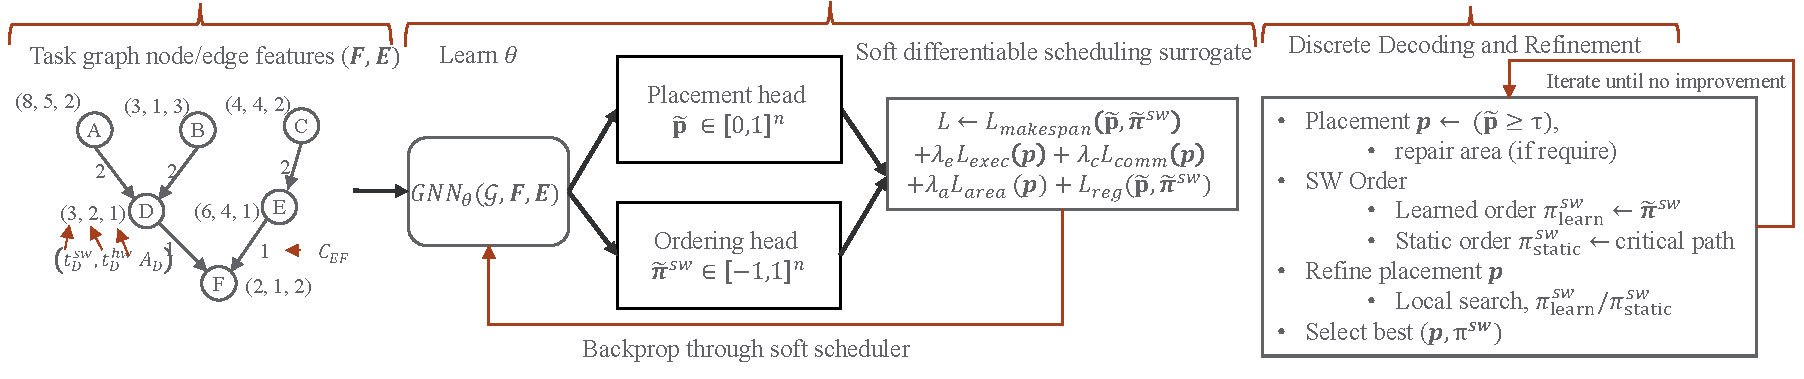
\includegraphics[width=1.0\linewidth]{Figures/methods/GNN_placement_order.pdf}
\caption{\sid{placeholder} Overview of \diffgnn for joint HW/SW partitioning and scheduling. A GNN encoder maps task graph features to the relaxed placement vector $\tilde{\vp}$ and relaxed software-priority vector $\tilde{\vpi}^{sw}$. A differentiable scheduling surrogate enables end-to-end optimization of makespan under constraints. At inference, solutions are discretized, repaired for feasibility, optionally refined, and evaluated using both the learned software order and a heuristic static-priority order; the better schedule is retained.}
\label{fig:diff_gnn_architecture}
\end{figure*}

\section{Proposed Method: \diffgnn}
\label{sec:method}

Building on the relaxed formulation in Section~\ref{sec:preliminaries}, we propose \diffgnn, a differentiable graph neural framework for jointly optimizing HW/SW partitioning and scheduling. Rather than directly searching over the discrete placement vector $\vp \in \{0,1\}^n$ and software order $\pi^{sw}$, \diffgnn learns a relaxed hardware-assignment vector $\tilde{\vp}\in[0,1]^n$ together with a relaxed software-priority vector $\tilde{\vpi}^{sw}\in[-1,1]^n$, and optimizes the relaxed objective in Equation~\eqref{eq:relaxed_obj} end-to-end using gradient-based learning.

Figure~\ref{fig:diff_gnn_architecture} illustrates the overall pipeline. Given a task graph $\gG(\gV,\gE)$, we first construct node and edge features, and a GNN encoder computes node embeddings that are then consumed by two prediction heads: (i) a \emph{placement head} that predicts relaxed hardware-assignment probabilities, and (ii) an \emph{ordering head} that predicts relaxed software priorities. These outputs are passed to an order-aware differentiable scheduler that approximates the makespan while accounting for both precedence constraints and software serialization. During inference, the relaxed solution is discretized, repaired if necessary to satisfy the area constraint, optionally refined, and finally evaluated using a discrete scheduler under two candidate software orders: the learned order induced by $\tilde{\vpi}^{sw}$ and a heuristic static-priority order. The better schedule is selected as the final output.


\subsection{Input Feature Preparation}

\paragraph{\textbf{Node features.}}
Each node $i \in \gV$ is associated with a feature vector capturing execution cost, resource usage, and structural properties:
\begin{equation}
\vf_i^{\mathrm{raw}} =
\left[
t_i^{sw},\;
t_i^{hw},\;
A_i,\;
d_i,\;
\frac{t_i^{hw}}{t_i^{sw}+\epsilon},\;
t_i^{sw}-t_i^{hw},\;
\frac{t_i^{sw}-t_i^{hw}}{\max(A_i,\epsilon)}
\right]
\in \mathbb{R}^7.
\end{equation}

Stacking all node features yields
\begin{equation}
\mF^{\mathrm{raw}} =
\begin{bmatrix}
(\vf_1^{\mathrm{raw}})^\top\\
\vdots\\
(\vf_n^{\mathrm{raw}})^\top
\end{bmatrix}
\in \mathbb{R}^{n\times 7}.
\end{equation}

We normalize features across nodes using column-wise z-score normalization:
\begin{equation}
\tilde{\mF} = \mathrm{Norm}(\mF^{\mathrm{raw}}).
\end{equation}

To incorporate the global hardware-area constraint, we append a constant feature:
\begin{equation}
\mF=
\begin{bmatrix}
\tilde{\mF} & \rho_A \mathbf{1}
\end{bmatrix}
\in\mathbb{R}^{n\times 8},
\end{equation}
where $\mathbf{1}\in\mathbb{R}^n$ is the all-ones vector.

\paragraph{\textbf{Edge features.}}
For each directed edge $(j,i)\in\gE$, we define an edge feature vector:
\begin{equation}
\ve_{ji}^{\mathrm{raw}} =
\left[
C_{ji},\;
|g_j-g_i|,\;
|ga_j-ga_i|
\right]
\in \mathbb{R}_{\ge 0}^3.
\end{equation}

Stacking all edges yields
\begin{equation}
\mE^{\mathrm{raw}} \in \mathbb{R}^{|\gE|\times 3}.
\end{equation}

We normalize edge features using column-wise max scaling:
\begin{equation}
\mE = \mathrm{Norm}_\infty(\mE^{\mathrm{raw}}),
\end{equation}
where $\mathrm{Norm}_\infty(\cdot)$ denotes feature-wise normalization by the maximum value.

\subsection{GNN Module}

\paragraph{\textbf{Message passing.}}
Let $\vh_i^{(0)}=\mF_{i,:}$ denote the initial node embedding. We use a message-passing GNN with $L$ layers:
\begin{equation}
\vh_i^{(\ell+1)}=
\phi^{(\ell)}\!\left(
\vh_i^{(\ell)},
\operatorname*{AGG}_{j:(j,i)\in\gE}
\psi^{(\ell)}\!\left(
\vh_i^{(\ell)},\;
\vh_j^{(\ell)},\;
\ve_{ji}
\right)
\right),
\end{equation}
for $\ell=0,\dots,L-1$, where $\phi^{(\ell)}$ and $\psi^{(\ell)}$ are learnable functions and $\operatorname*{AGG}$ is a permutation-invariant aggregation operator.

As a concrete instantiation, we use weighted mean aggregation:
\begin{align*}
\operatorname*{AGG}_{j:(j,i)\in\gE}
\psi^{(\ell)}\!\left(
\vh_i^{(\ell)},\;
\vh_j^{(\ell)},\;
\ve_{ji}
\right)
&=\frac{1}{\alpha}\sum_{j\in\gN(i)}\alpha_{\phi}(j,i)\,\mathbf{W}^{(\ell)}\vh_j^{(\ell)},\\
\alpha &= \sum_{j\in\gN(i)} \alpha_{\phi}(j,i)+\epsilon,
\end{align*}
where $\gN(i)$ denotes the set of incoming neighbors of node $i$, $\mathbf{W}^{(\ell)}$ is a learnable linear transformation, and $\alpha_{\phi}(j,i)\ge 0$ is a learnable edge weight derived from $\ve_{ji}$. We compute
\begin{equation}
\alpha_{\phi}(j,i)=\sigma\!\left(f_{\phi}(\ve_{ji})\right),
\end{equation}
where $f_{\phi}$ is an MLP and $\sigma(\cdot)$ is the sigmoid function.

\paragraph{\textbf{Placement head.}}
From the final embedding $\vh_i^{(L)}$, we predict relaxed hardware-assignment probabilities:
\begin{equation}
\tilde{p}_i = \sigma\!\left(\mathrm{MLP}_{\mathrm{place}}(\vh_i^{(L)})\right),
\end{equation}
where $\sigma(\cdot)$ denotes the sigmoid function, ensuring $\tilde{p}_i\in(0,1)$. Stacking all node-wise predictions gives
\begin{equation}
\tilde{\vp} = [\tilde{p}_1,\dots,\tilde{p}_n]^\top .
\end{equation}

\paragraph{\textbf{Ordering head.}}
To model software execution order, we compute bounded relaxed software-priority values:
\begin{equation}
\tilde{\pi}_i^{sw} = \tanh\!\left(\mathrm{MLP}_{\mathrm{order}}(\vh_i^{(L)})\right),
\end{equation}
so that $\tilde{\pi}_i^{sw}\in(-1,1)$. Stacking them yields
\begin{equation}
\tilde{\vpi}^{sw} = [\tilde{\pi}_1^{sw},\dots,\tilde{\pi}_n^{sw}]^\top \in \mathbb{R}^n.
\end{equation}


\subsection{Differentiable Soft Scheduler}

We now instantiate the relaxed makespan term $\widetilde{M}(\tilde{\vp},\tilde{\vpi}^{sw})$ from Section~\ref{sec:preliminaries}. The scheduler takes as input the relaxed placement vector $\tilde{\vp}$ and the relaxed software-priority vector $\tilde{\vpi}^{sw}$, and produces approximate start and finish times for all tasks.

The most important intermediate quantity is the effective software-order matrix $R^{sw}$. Figure~\ref{fig:soft_scheduler_walkthrough} illustrates its construction on a 6-node example. Read the figure from left to right:
\[
\tilde{\vpi}^{sw}
\;\rightarrow\;
\mP^{sw}
\;\rightarrow\;
\tilde{\vr}
\;\rightarrow\;
\mB^{sw}
\;\rightarrow\;
\mR^{sw}
\;\rightarrow\;
\widetilde{M}(\tilde{\vp},\tilde{\vpi}^{sw}).
\]

\begin{figure*}[t]
\centering
\setlength{\tabcolsep}{2.2pt}
\renewcommand{\arraystretch}{1.0}
\begin{adjustbox}{width=\textwidth,center}
\begin{tikzpicture}[
    >=Latex,
    font=\scriptsize,
    box/.style={draw=black!55, rounded corners=1pt, fill=gray!5, inner sep=2.2pt, align=center},
    arr/.style={-{Latex[length=1.8mm]}, very thick, draw=orange!85!black}
]

% =========================================================
% 1) GRAPH + INPUTS
% =========================================================
\node[anchor=north west] (graphbox) at (0,0) {%
\begin{minipage}{0.20\textwidth}
\centering
\begin{tikzpicture}[scale=0.68, every node/.style={font=\scriptsize}]
\node[circle,draw,fill=orange!85!yellow,inner sep=1.6pt,label=above:{A $(8,5,2)$}] (A) at (0,1.8) {};
\node[circle,draw,fill=orange!85!yellow,inner sep=1.6pt,label=above:{B $(3,1,3)$}] (B) at (1.9,1.8) {};
\node[circle,draw,fill=orange!85!yellow,inner sep=1.6pt,label=above:{C $(4,4,2)$}] (C) at (3.8,1.8) {};
\node[circle,draw,fill=black!90,inner sep=1.6pt,label=left:{D $(3,2,1)$}] (D) at (0.95,0.7) {};
\node[circle,draw,fill=black!90,inner sep=1.6pt,label=right:{E $(6,4,1)$}] (E) at (2.85,0.7) {};
\node[circle,draw,fill=black!90,inner sep=1.6pt,label=below:{F $(2,1,2)$}] (F) at (1.90,-0.35) {};
\draw[->,thin] (A)-- node[left] {\scriptsize 2} (D);
\draw[->,thin] (B)-- node[left] {\scriptsize 2} (D);
\draw[->,thin] (C)-- node[right] {\scriptsize 2} (E);
\draw[->,thin] (D)-- node[below] {\scriptsize 0} (F);
\draw[->,thin] (E)-- node[below] {\scriptsize 0} (F);
\end{tikzpicture}

\vspace{0.8mm}
$\tilde{\vp}=[0.05,0.05,0.05,0.95,0.95,0.95]^\top$

$\tilde{\vpi}^{sw}=[0.00,-1.00,1.00,-0.50,-0.75,-0.25]^\top$

Induced SW order: $C \prec A \prec B$
\end{minipage}
};

% =========================================================
% 2) ORDER VECTOR
% =========================================================
\node[box, anchor=north west] (qtab) at (4.25,0) {%
\begin{tabular}{c|c}
Task & $\tilde{\pi}^{sw}$\\\hline
A & \textcolor{red}{0.00}\\
B & \textcolor{red}{-1.00}\\
C & \textcolor{red}{1.00}\\
D & -0.50\\
E & -0.75\\
F & -0.25
\end{tabular}
};

% =========================================================
% 3) SINKHORN MATRIX
% =========================================================
\node[box, anchor=north west] (pmat) at (6.15,0) {%
\begin{tabular}{c|cccccc}
$u_a$ & A & B & C & D & E & F\\\hline
1.0  & 0.181 & 0.002 & \textcolor{red}{0.695} & 0.029 & 0.008 & 0.084\\
0.6  & \textcolor{red}{0.332} & 0.015 & 0.257 & 0.120 & 0.047 & 0.229\\
0.2  & 0.271 & 0.060 & 0.043 & 0.218 & 0.128 & 0.280\\
-0.2 & 0.143 & 0.155 & 0.005 & 0.255 & 0.224 & 0.219\\
-0.6 & 0.056 & 0.302 & 0.000 & 0.223 & 0.291 & 0.128\\
-1.0 & 0.017 & \textcolor{red}{0.467} & 0.000 & 0.155 & 0.302 & 0.060
\end{tabular}
};

\node[font=\scriptsize] at ($(pmat.south)+(0,-0.28)$)
{$L_{ai}=-(\tilde{\pi}^{sw}_i-u_a)^2/\tau_o,\quad \mP^{sw}=\mathrm{Sinkhorn}(L)$};

% =========================================================
% 4) RANK TABLE
% =========================================================
\node[box, anchor=north west] (rtab) at (11.10,0) {%
\begin{tabular}{c|c}
Task & $\tilde r_i$\\\hline
A & \textcolor{red}{1.613}\\
B & \textcolor{red}{4.141}\\
C & \textcolor{red}{0.357}\\
D & 2.986\\
E & 3.649\\
F & 2.258
\end{tabular}
};

\node[font=\scriptsize] at ($(rtab.south)+(0,-0.28)$)
{$\tilde r_i=\sum_{a=0}^{n-1} a\,\mP^{sw}_{ai}$};

% =========================================================
% 5) COMBINED GATE + BEFORE BOX
% =========================================================
\node[box, anchor=north west] (gbbox) at (13.00,0) {%
\begin{minipage}{0.23\textwidth}
\centering
$\displaystyle
G^{sw}=(1-\tilde{\vp})(1-\tilde{\vp})^\top=
\begin{bmatrix}
0.903\,\mathbf{1}_{3\times3} & 0.048\,\mathbf{1}_{3\times3}\\
0.048\,\mathbf{1}_{3\times3} & 0.003\,\mathbf{1}_{3\times3}
\end{bmatrix}
$

\vspace{0.8mm}
\begin{tabular}{c|cccccc}
 & A & B & C & D & E & F\\\hline
A & 0     & 0.999 & 0.027 & 0.981 & 0.997 & 0.863\\
B & 0.001 & 0     & 0     & 0.036 & 0.197 & 0.005\\
C & \textcolor{red}{0.973} & \textcolor{red}{1.000} & 0 & 0.999 & 1.000 & 0.996\\
D & 0.019 & 0.964 & 0.001 & 0 & 0.869 & 0.111\\
E & 0.003 & 0.803 & 0 & 0.131 & 0 & 0.018\\
F & 0.137 & 0.995 & 0.004 & 0.889 & 0.982 & 0
\end{tabular}

\vspace{0.6mm}
$\displaystyle B^{sw}_{ji}=\sigma\!\left(\frac{\tilde r_i-\tilde r_j}{\tau_r}\right)$
\end{minipage}
};

% =========================================================
% 6) FINAL RESOURCE MATRIX
% =========================================================
\node[box, anchor=north west] (rmat) at (18.00,0) {%
\begin{tabular}{c|cccccc}
 & A & B & C & D & E & F\\\hline
A & 0     & 0.902 & \textcolor{red}{0.024} & 0.047 & 0.047 & 0.041\\
B & 0.001 & 0     & 0     & 0.002 & 0.009 & 0\\
C & \textcolor{red}{0.878} & \textcolor{red}{0.902} & 0 & 0.047 & 0.047 & 0.047\\
D & 0.001 & 0.046 & 0 & 0 & 0.002 & 0\\
E & 0 & 0.038 & 0 & 0 & 0 & 0\\
F & 0.006 & 0.047 & 0 & 0.002 & 0.002 & 0
\end{tabular}
};

\node[font=\scriptsize] at ($(rmat.south)+(0,-0.28)$)
{$R^{sw}=B^{sw}\odot G^{sw}$};

\node[font=\scriptsize] at ($(rmat.south)+(0,-0.68)$)
{Key entries: $R^{sw}_{CA}=0.878,\;R^{sw}_{CB}=0.902,\;R^{sw}_{AB}=0.902$};

% =========================================================
% 7) MAKESPAN BOX
% =========================================================
\node[anchor=north west] (mspan) at (22.65,0) {%
\begin{minipage}{0.27\textwidth}
\centering
\textbf{From $R^{sw}$ to relaxed makespan}

\vspace{0.8mm}
Using the induced order $C \prec A \prec B$:
\[
\tilde f_C=4.00,\quad \tilde f_A=11.85,\quad \tilde f_B=14.75
\]
\[
\tilde s_D=16.55,\ \tilde f_D=18.60,\qquad
\tilde s_E=5.80,\ \tilde f_E=9.90
\]
\[
\tilde s_F=18.60,\qquad \tilde f_F=19.65
\]
\[
\widetilde{M}(\tilde{\vp},\tilde{\vpi}^{sw})
=
\mathrm{SMax}_{\beta}\!\big(\{\tilde f_i:i\in\Sink(\gG)\}\big)
\approx 19.65
\]

Alternative order $A \prec B \prec C$:
\[
\tilde f_F\approx 21.70
\]
Hence the learned ordering reduces the relaxed makespan.
\end{minipage}
};

% =========================================================
% ARROWS
% =========================================================
\draw[arr] (graphbox.east) -- (qtab.west);
\draw[arr] (qtab.east) -- (pmat.west);
\draw[arr] (pmat.east) -- (rtab.west);
\draw[arr] (rtab.east) -- (gbbox.west);
\draw[arr] (gbbox.east) -- (rmat.west);
\draw[arr] (rmat.east) -- (mspan.west);

\end{tikzpicture}
\end{adjustbox}
\caption{Numerical walk-through of the soft scheduler on a 6-node example. The example graph and relaxed inputs are followed by the ordering vector, Sinkhorn soft permutation matrix, expected ranks, gated rank-based precedence structure, effective software-order matrix $R^{sw}$, and the resulting relaxed makespan computation. The highlighted entries show that the example strongly favors the software order $C \prec A \prec B$.}
\label{fig:soft_scheduler_walkthrough}
\end{figure*}
First, the ordering head predicts relaxed software priorities $\tilde{\vpi}^{sw}$. These values are converted into a soft permutation matrix $\mP^{sw}$ using Sinkhorn normalization; $\mP^{sw}$ is then mapped to expected ranks $\tilde r_i$; the ranks are converted into a pairwise before matrix $\mB^{sw}$; and finally $\mB^{sw}$ is gated by the software co-assignment matrix so that ordering affects only tasks that are likely mapped to software. The same figure then shows how the resulting order propagates to the relaxed start and finish times and, ultimately, to the relaxed makespan.

\paragraph{\textbf{From relaxed software priorities to the effective software-order matrix.}}
The ordering head outputs
\begin{equation}
\tilde{\vpi}^{sw}=[\tilde{\pi}_1^{sw},\ldots,\tilde{\pi}_n^{sw}]^\top.
\end{equation}
We first construct a score-to-position compatibility matrix
\begin{equation}
L_{ai}=-\frac{(\tilde{\pi}_i^{sw}-u_a)^2}{\tau_o},
\qquad
u_a=1-\frac{2a}{n-1},
\quad a=0,\ldots,n-1,
\end{equation}
where $\{u_a\}_{a=0}^{n-1}$ are evenly spaced position anchors and $\tau_o$ controls the sharpness of the relaxation. Applying Sinkhorn normalization gives
\begin{equation}
\mP^{sw}=\mathrm{Sinkhorn}(L)\in[0,1]^{n\times n},
\end{equation}
where $\mP^{sw}_{ai}$ is the soft probability that task $i$ occupies position $a$ in the software order.

Next we compute the expected rank of each task:
\begin{equation}
\tilde r_i=\sum_{a=0}^{n-1} a\,\mP^{sw}_{ai}.
\end{equation}
A smaller $\tilde r_i$ indicates that task $i$ is predicted to execute earlier on software. We then convert these ranks into pairwise precedence scores:
\begin{equation}
B^{sw}_{ji}
=
\sigma\!\left(\frac{\tilde r_i-\tilde r_j}{\tau_r}\right),
\qquad
B^{sw}_{ii}=0,
\end{equation}
so that $B^{sw}_{ji}$ is large when task $j$ is likely to execute before task $i$.

Since ordering matters only when both tasks are likely assigned to software, we gate the pairwise precedence by
\begin{equation}
G^{sw}=(1-\tilde{\vp})(1-\tilde{\vp})^\top,
\end{equation}
and define the effective software-order matrix
\begin{equation}
R^{sw}_{ji}=B^{sw}_{ji}(1-\tilde{p}_j)(1-\tilde{p}_i)
\;=\;
B^{sw}_{ji}G^{sw}_{ji}.
\end{equation}
Thus, $R^{sw}_{ji}$ is large only when task $j$ is likely to precede task $i$ \emph{and} both tasks are likely mapped to software. In the example of Figure~\ref{fig:soft_scheduler_walkthrough}, this gives large entries such as $R^{sw}_{CA}=0.878$, $R^{sw}_{CB}=0.902$, and $R^{sw}_{AB}=0.902$, which strongly favor the software order $C\prec A\prec B$.

\paragraph{\textbf{Relaxed execution and communication.}}
The relaxed execution time of node $i$ is
\begin{equation}
\tilde{t}_i(\tilde{\vp})=\tilde{p}_i t_i^{hw} + (1-\tilde{p}_i)t_i^{sw},
\end{equation}
and the relaxed communication delay on edge $(j,i)$ is
\begin{equation}
\tilde{c}_{ji}(\tilde{\vp})=|\tilde{p}_j-\tilde{p}_i|\,C_{ji}.
\end{equation}

\paragraph{\textbf{DAG readiness.}}
Let $\Pred(i)$ denote the set of predecessors of node $i$. The DAG-readiness term is
\begin{equation}
s_i^{dag}
=
\begin{cases}
0, & \Pred(i)=\emptyset,\\[4pt]
\mathrm{SMax}_{\beta}
\Big(
\{\, \tilde{f}_j + \tilde{c}_{ji}(\tilde{\vp}) \mid j \in \Pred(i)\,\}
\Big), & \text{otherwise},
\end{cases}
\end{equation}
where
\begin{equation}
\mathrm{SMax}_{\beta}(\{a_k\})=\frac{1}{\beta}\log\sum_k e^{\beta a_k}.
\end{equation}
Intuitively, $s_i^{dag}$ is the earliest soft time at which task $i$ becomes ready from the precedence perspective.

\paragraph{\textbf{Software readiness.}}
Because software tasks execute sequentially on a single CPU, task $i$ may also need to wait for software tasks predicted to execute before it. We model this using $R^{sw}$:
\begin{equation}
\phi_{sw}(\tilde{\pi}_j^{sw},\tilde{\pi}_i^{sw})
=
\alpha \log(R^{sw}_{ji}+\epsilon),
\end{equation}
and define the software-readiness term as
\begin{equation}
s_i^{sw}
=
\mathrm{SMax}_{\beta}
\Big(
\{\, \tilde{f}_j + \phi_{sw}(\tilde{\pi}_j^{sw},\tilde{\pi}_i^{sw}) \mid j \neq i\,\}
\Big).
\end{equation}
If $R^{sw}_{ji}$ is large, then task $j$ is likely to delay task $i$ on the software processor.

\paragraph{\textbf{Start and finish times.}}
The relaxed start time of node $i$ is obtained by combining DAG and software readiness:
\begin{equation}
\tilde{s}_i=\mathrm{SMax}_{\beta}\big(\{s_i^{dag},\,s_i^{sw}\}\big),
\end{equation}
and the corresponding relaxed finish time is
\begin{equation}
\tilde{f}_i=\tilde{s}_i+\tilde{t}_i(\tilde{\vp}).
\end{equation}

\paragraph{\textbf{Soft makespan.}}
Let $\Sink(\gG)$ denote the set of sink nodes in $\gG$. The relaxed makespan is
\begin{equation}
L_{\mathrm{soft\mbox{-}makespan}}(\tilde{\vp},\tilde{\vpi}^{sw})
=
\widetilde{M}(\tilde{\vp},\tilde{\vpi}^{sw})
=
\mathrm{SMax}_{\beta}\big(\{\, \tilde{f}_i \mid i \in \Sink(\gG)\,\}\big).
\end{equation}

Figure~\ref{fig:soft_scheduler_walkthrough} also shows why the induced order $C\prec A\prec B$ is useful in this example: it starts the $C\!\rightarrow\!E$ branch earlier, which reduces the final relaxed makespan. Appendix~\ref{app:illustration} provides the full numerical walk-through of the resulting start and finish times.

\subsection{Training Objective}

The base relaxed objective is given in Equation~\eqref{eq:relaxed_obj}. In practice, we augment it with auxiliary execution, communication, and regularization terms:
\begin{equation}
L
=
L_{\mathrm{makespan}}(\tilde{\vp},\tilde{\vpi}^{sw})
+
\lambda_e L_{\mathrm{exec}}(\tilde{\vp})
+
\lambda_c L_{\mathrm{comm}}(\tilde{\vp})
+
\lambda_a L_{\mathrm{area}}(\tilde{\vp})
+
L_{\mathrm{reg}}(\tilde{\vp},\tilde{\vpi}^{sw}).
\end{equation}

Here, $L_{\mathrm{makespan}}$ captures the differentiable scheduling objective, while $L_{\mathrm{exec}}$ and $L_{\mathrm{comm}}$ correspond to relaxed execution and communication costs, respectively.

\paragraph{\textbf{Execution and communication losses.}}
We directly treat the relaxed execution and communication terms as auxiliary losses:
\begin{equation}
L_{\mathrm{exec}}(\tilde{\vp}) = \sum_{i\in\gV}\tilde{t}_i(\tilde{\vp}),
\qquad
L_{\mathrm{comm}}(\tilde{\vp}) = \sum_{(j,i)\in\gE}\tilde{c}_{ji}(\tilde{\vp}).
\end{equation}

The execution and communication terms regularize the optimization by discouraging slow assignments and excessive cross-partition communication, thereby aiding makespan minimization.

\paragraph{\textbf{Area constraint.}}
To enforce the hardware budget during training, we replace the hard constraint with a differentiable hinge penalty:
\begin{equation}
L_{\mathrm{area}}(\tilde{\vp})
=
\left[
\max\!\left(
0,\sum_{i\in\gV}\tilde{p}_i A_i - A_{\max}
\right)
\right]^2.
\end{equation}

\paragraph{\textbf{Regularization.}}
We further introduce optional regularization to stabilize ordering predictions and encourage nearly discrete assignments:
\begin{equation}
L_{\mathrm{reg}}(\tilde{\vp},\tilde{\vpi}^{sw})
=
\lambda_b L_{\mathrm{binary}}(\tilde{\vp})
+
\lambda_p L_{\mathrm{perm}}(\mP^{sw}),
% +
% \lambda_u L_{\mathrm{usage}}(\tilde{\vp}),
\end{equation}
where
\begin{align}
L_{\mathrm{binary}}(\tilde{\vp})
&=
\frac{1}{n}\sum_{i=1}^n \tilde{p}_i(1-\tilde{p}_i),\\
L_{\mathrm{p}}(\mP^{sw})
&=
\|\mP^{sw}\mathbf{1}-\mathbf{1}\|_2^2
+
\|(\mP^{sw})^\top\mathbf{1}-\mathbf{1}\|_2^2,
\\
% L_{\mathrm{usage}}(\tilde{\vp})
% &=
% (\mu_p-\rho)^2,
% \qquad
% \mu_p=\frac{1}{n}\sum_{i=1}^n \tilde{p}_i.
\end{align}

The term $L_{\mathrm{binary}}$ pushes relaxed assignments toward discrete decisions. 
The term $L_{\mathrm{perm}}$ keeps the soft ordering matrix close to a valid permutation relaxation. 
% The term $L_{\mathrm{usage}}$ controls the overall hardware usage level by matching the mean assignment to a target ratio $\rho$.

\subsection{Discrete Inference: Decoding, Scheduling, and Refinement}
\label{subsec:inference}

The outputs of \diffgnn are converted into a feasible discrete solution through a discrete inference pipeline. This stage bridges the gap between the differentiable training surrogate and the final discrete scheduling objective.

\paragraph{\textbf{Decoding and candidate generation.}}
Given relaxed placement probabilities $\tilde{\vp}$, we generate a set of discrete candidate partitions by thresholding:
\begin{equation}
\hat{p}_i = \mathbb{I}[\tilde{p}_i \ge \tau_d], \qquad \tau_d \in \mathcal{T},
\end{equation}
where $\mathcal{T}$ is a set of decoding thresholds.

\paragraph{\textbf{Feasibility repair.}}
Decoded candidates may violate the hardware area constraint. For each candidate, we enforce feasibility:
\begin{equation}
\sum_{i \in \gV} \hat{p}_i A_i \le A_{\max}.
\end{equation}
When the area constraint is violated, we run a deterministic repair loop: we repeatedly move one task from hardware to software, choosing the hardware task with the lowest benefit-per-area priority. This continues until the hardware area is within budget, thereby guaranteeing feasibility. After that, if area remains, we optionally test software-to-hardware flips that still fit the remaining area and keep the move with the best makespan improvement; by default, only non-worsening moves are accepted.

\paragraph{\textbf{Software order computation.}}
For each feasible decoded placement $\hat{\vp}$, we construct two candidate software orders. The first is the \emph{learned order} $\pi_{\mathrm{learn}}^{sw}$, obtained by sorting the relaxed software-priority vector $\tilde{\vpi}^{sw}$. The second is the \emph{static-priority order} $\pi_{\mathrm{static}}^{sw}$, computed using the same critical-path priority rule as LSSP on the decoded placement $\hat{\vp}$. Specifically, let
\begin{equation}
t_i(\hat{\vp}) = \hat{p}_i t_i^{hw} + (1-\hat{p}_i)t_i^{sw},
\end{equation}
and
\begin{equation}
\mathrm{comm}_{ij}(\hat{\vp}) = \mathbb{I}[\hat{p}_i \neq \hat{p}_j]\, C_{ij}.
\end{equation}
The static priority of task $i$ is computed in reverse topological order as
\begin{equation}
\mathrm{Pri}(i)
=
t_i(\hat{\vp})
+
\max_{j\in \Succ(i)}
\left(
\mathrm{comm}_{ij}(\hat{\vp}) + \mathrm{Pri}(j)
\right),
\label{eq:lssp_priority}
\end{equation}
with $\mathrm{Pri}(i)=t_i(\hat{\vp})$ for sink tasks. Intuitively, $\mathrm{Pri}(i)$ estimates how critical task $i$ is to the final makespan. Figure~\ref{fig:staticpriorities} illustrates how these priorities are computed bottom-up. If there are multiple sink nodes, we add a dummy sink node and start the computation from there.

\begin{figure}[!htbp]
\centering
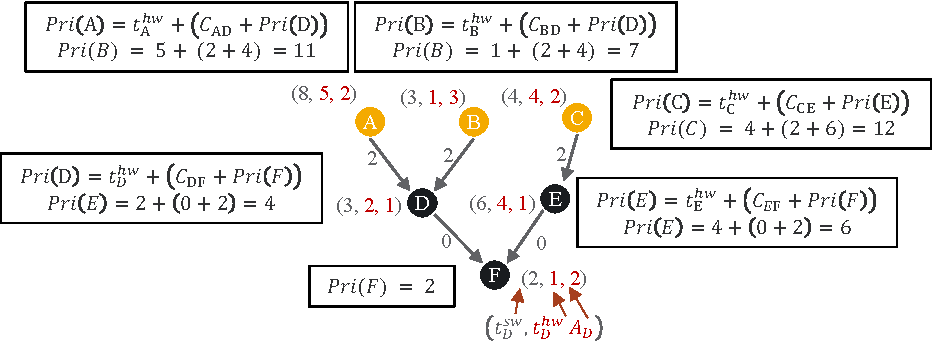
\includegraphics[width=1.0\linewidth]{Figures/methods/static_priorities.pdf}
\caption{\sid{placeholder} Example of bottom-up static-priority computation.}
\label{fig:staticpriorities}
\end{figure}

\paragraph{\textbf{Makespan computation.}}
Given a discrete placement $\hat{\vp}$, we run list scheduling twice, once with software order $\pi_{\mathrm{learn}}^{sw}$ and once with $\pi_{\mathrm{static}}^{sw}$. Let $k \in \{\mathrm{learn},\mathrm{static}\}$ denote the chosen software-order policy. At each scheduling event $t$, the next software task is selected from the ready software set
\begin{equation}
\mathcal{R}_{sw}(t)=\{i\mid \hat{p}_i=0,\ \Pred(i)\subseteq \mathcal{C}(t)\},
\qquad
i_t^{(k)}=\arg\max_{i\in\mathcal{R}_{sw}(t)} \pi_k^{sw}(i),
\end{equation}
with deterministic tie-breaking. Dependency readiness is
\begin{equation}
r_i^{(k)}=\max_{j\in\Pred(i)}\big(f_j^{(k)}+c_{ji}(\hat{\vp})\big),
\end{equation}
and start/finish times are
\begin{equation}
s_i^{(k)}=\max\!\big(r_i^{(k)},t_{i,\mathrm{avail}}^{(k)}\big),
\qquad
f_i^{(k)}=s_i^{(k)}+t_i(\hat{\vp}),
\end{equation}
where
\begin{equation}
t_{i,\mathrm{avail}}^{(k)}=
\begin{cases}
t_{SW,\mathrm{avail}}^{(k)}, & \hat{p}_i=0,\\
0, & \hat{p}_i=1,
\end{cases}
\end{equation}
and $t_{SW,\mathrm{avail}}^{(k)}$ is the current availability time of the single software lane, updated after each scheduled software task.

This yields two candidate makespans,
\begin{equation}
T^{\mathrm{learn}}=\max_i f_i^{(\mathrm{learn})},
\qquad
T^{\mathrm{static}}=\max_i f_i^{(\mathrm{static})}.
\end{equation}
For \diffgnn, we define the discrete evaluation score of placement $\hat{\vp}$ as
\begin{equation}
T^\star(\hat{\vp})
=
\min\!\big(T^{\mathrm{learn}},\,T^{\mathrm{static}}\big),
\label{eq:best_of_two_orders}
\end{equation}
and denote the corresponding selected software order by $\hat{\pi}^{sw}$.

\paragraph{\textbf{Optional local refinement.}}
Starting from the repaired placement, we optionally apply local search to explore local changes, such as flipping assignments of critical nodes. Each proposed move is evaluated using the discrete makespan score $T^\star(\hat{\vp})$, and a move is accepted only if it improves the current solution under this evaluation.

\paragraph{\textbf{Final selection.}}
Across all decoded candidates and their refined versions, we select the solution with the smallest final discrete makespan:
\begin{equation}
(\vp^\star,\pi^{sw,\star})
=
\arg\min_{(\hat{\vp},\hat{\pi}^{sw})\in\mathcal{C}}
M(\hat{\vp},\hat{\pi}^{sw}),
\end{equation}
where $\mathcal{C}$ denotes the set of all feasible decoded or refined placements together with their selected software orders. Equivalently, the final makespan reported for \diffgnn is the minimum value of $T^\star(\hat{\vp})$ over all candidates.

For competing algorithms, we use only the LS-based static-priority order, so that all baselines are evaluated under the same standard discrete scheduling rule.




\subsection{Pseudocode of \diffgnn}
Algorithms~\ref{alg:diffgnn_training} and~\ref{alg:diffgnn_inference} summarize the training and discrete inference procedures of \diffgnn.

\begin{algorithm}[!htbp]
\caption{Training of \diffgnn}
\label{alg:diffgnn_training}
\KwIn{Task graph $\gG=(\gV,\gE)$, epochs $T$, area budget $A_{\max}$}
\KwIn{Loss weights $\lambda_e,\lambda_c,\lambda_a,\lambda_b,\lambda_p$}
\KwIn{Temperatures $\tau_o,\tau_r$ and smooth-max parameter $\beta$}
Initialize model parameters $\theta$\;
Construct node and edge features $\mF,\mE$\;

\For{$t=1,\dots,T$}{
    Predict $\tilde{\vp},\tilde{\vpi}^{sw}\gets \mathrm{GNN}_{\theta}(\gG,\mF,\mE)$\;
    
    Build soft precedence from $\tilde{\vpi}^{sw}$ using Sinkhorn relaxation\;
    
    Compute relaxed execution/communication terms $\tilde{t}_i,\tilde{c}_{ji}$\;
    
    Run differentiable scheduler to obtain $\tilde{\vs},\tilde{\vf}$\;
    
    Compute $L_{\mathrm{makespan}},L_{\mathrm{exec}},L_{\mathrm{comm}},L_{\mathrm{area}},L_{\mathrm{reg}}$\;
    
    $L \gets L_{\mathrm{makespan}}
    + \lambda_e L_{\mathrm{exec}}
    + \lambda_c L_{\mathrm{comm}}
    + \lambda_a L_{\mathrm{area}}
    + L_{\mathrm{reg}}$\;
    
    Update $\theta$ via backpropagation\;
}
\end{algorithm}

\begin{algorithm}[!htbp]
\caption{Discrete Inference and Post-Processing}
\label{alg:diffgnn_inference}
\KwIn{Graph $\gG$, trained model, area budget $A_{\max}$, thresholds $\mathcal{T}$}
\KwOut{Best discrete placement $\vp^\star$, software order $\pi^{sw,\star}$, makespan $M^\star$}

Compute $\tilde{\vp},\tilde{\vpi}^{sw}$\;
Initialize $\vp^\star \gets \emptyset$, $\pi^{sw,\star}\gets\emptyset$, $M^\star \gets +\infty$\;

\For{$\tau_d \in \mathcal{T}$}{
    Decode $\hat{\vp}$ by thresholding:
    $\hat{p}_i \gets \mathbb{I}[\tilde{p}_i \ge \tau_d]$\;
    
    Repair $\hat{\vp}$ until $\sum_i \hat{p}_i A_i \le A_{\max}$\;
    
    Refine $\hat{\vp}$ using local search\tcp*[r]{optional}
    
    Compute learned software order $\pi_{\mathrm{learn}}^{sw}$ by sorting $\tilde{\vpi}^{sw}$\;
    Compute static-priority order $\pi_{\mathrm{static}}^{sw}$ on $\hat{\vp}$\;
    
    $T^{\mathrm{learn}} \gets M(\hat{\vp},\pi_{\mathrm{learn}}^{sw})$,
    $T^{\mathrm{static}} \gets M(\hat{\vp},\pi_{\mathrm{static}}^{sw})$\;
    
    $\hat{\pi}^{sw} \gets
    \arg\min_{\pi \in \{\pi_{\mathrm{learn}}^{sw},\,\pi_{\mathrm{static}}^{sw}\}}
    M(\hat{\vp},\pi)$\;
    
    $T^\star(\hat{\vp}) \gets
    \min\!\big(T^{\mathrm{learn}},\,T^{\mathrm{static}}\big)$\;
    
    \If{$T^\star(\hat{\vp}) < M^\star$}{
        $\vp^\star \gets \hat{\vp}$,\quad
        $\pi^{sw,\star} \gets \hat{\pi}^{sw}$,\quad
        $M^\star \gets T^\star(\hat{\vp})$\;
    }
}
\Return{$(\vp^\star,\pi^{sw,\star},M^\star)$}\;
\end{algorithm}




\subsection{Complexity Analysis}

\paragraph{\textbf{Training Complexity.}}
Let $n=|\gV|$, $m=|\gE|$, hidden size $d$, and $L$ GNN layers. The GNN and prediction heads incur a cost of $O\!\big(L(md + nd^2)\big) + O(nd)$. Applying Sinkhorn normalization to an $n \times n$ matrix costs $O(T_{\mathrm{sink}} n^2)$, where $T_{\mathrm{sink}}$ (typically $10$--$12$) is the number of normalization iterations, and computing rank-based pairwise precedence requires $O(n^2)$. The differentiable scheduler adds $O(m + n^2)$.

Thus, the total time complexity per forward pass is $T_{\text{total}} = O\!\big(L(md + nd^2) + m + T_{\mathrm{sink}} n^2 + n^2\big)$. The space complexity is $S_{\text{total}} = O(Lnd + m + n^2)$, where the $n^2$ term (dense ordering tensors) is the primary scalability bottleneck.


\paragraph{\textbf{Post-processing complexity.}}
For each decoded placement, post-processing requires computing the learned software order, the static-priority order, and evaluating discrete schedules under both. The overall cost per decoded placement is $O(m+n\log n)$. Thus, with $|\mathcal{T}|$ decoding thresholds and $R$ local-refinement evaluations, the total post-processing complexity is $O\!\big((|\mathcal{T}|+R)(m+n\log n)\big)$. In practice, this is much smaller than the training cost.

\paragraph{\textbf{Large-graph approximation.}}
For large-scale graphs, we improve scalability by skipping Sinkhorn normalization and directly using ordering logits for pairwise precedence, while restricting software ordering to the top-$k$ high-confidence nodes per task. This reduces pairwise interactions from $O(n^2)$ to $O(nk)$ with $k \ll n$, yielding $T_{\text{total}} = O\!\big(L(md+nd^2)+m+nk\big)$ and $S_{\text{total}} = O(Lnd+m+nk)$.
\section{Experiments}
In this section, we answer the following questions.
\subsection{Dataset and settings}

\subsection{Makespan comparison}

% random: DAG 32, LSSP 32, SWPRIO -, BEST 32
% greedy: DAG 32, LSSP 32, SWPRIO -, BEST 32
% diff_gnn: DAG 31, LSSP 31, SWPRIO -, BEST 31
% diff_gnn_order: DAG 31, LSSP 31, SWPRIO 29, BEST 29
% gcps: DAG 32, LSSP 32, SWPRIO -, BEST 32
% pso: DAG 83, LSSP 83, SWPRIO -, BEST 83
% dbpso: DAG 29, LSSP 29, SWPRIO -, BEST 29
% clpso: DAG 30, LSSP 30, SWPRIO -, BEST 30
% ccpso: DAG 32, LSSP 32, SWPRIO -, BEST 32
% esa: DAG 30, LSSP 30, SWPRIO -, BEST 30
% shade: DAG 29, LSSP 29, SWPRIO -, BEST 29
% jade: DAG 29, LSSP 29, SWPRIO -, BEST 29
% gl25: DAG 29, LSSP 29, SWPRIO -, BEST 29

\subsection{Ablation Studies}
Base GNN, +sw ordering head, +hw ordering head, +post processing, +greedy fixing, +dag/lssp, +edge weight learning, +features, +objective functions 





\input{7Conclusion}

% \section{Method: Scheduling Objectives (Hard Baselines and Differentiable Surrogates)}
\label{sec:method}

% Requires in preamble:
% \usepackage{algorithm}
% \usepackage{algpseudocode}
% \usepackage{amsmath,amssymb}

%%%%%%%%%%%%%%%%%%%%%%%%%%%%%%%%%%%%%%%%%%%%%%%%%%%%%%%%%%%%%%%%%%%%%%%%%%%%%%
% Notation (shared by all pseudocodes)
%%%%%%%%%%%%%%%%%%%%%%%%%%%%%%%%%%%%%%%%%%%%%%%%%%%%%%%%%%%%%%%%%%%%%%%%%%%%%%
% DAG: G=(V,E), tasks i \in V, edges (u,i) \in E.
% Placement:
%   Hard: x[i] \in {SW, HW}
%   Soft: p_hw[i] \in [0,1], p_sw[i] = 1 - p_hw[i]
% Exec times: t_sw[i], t_hw[i]
% Comm: c[u,i] (paid iff lanes differ)
% Outputs: start s[i], finish f[i], makespan T
%
% Soft operators:
%   SoftMax_beta({z_k}) = (1/beta) log \sum_k exp(beta z_k)

%%%%%%%%%%%%%%%%%%%%%%%%%%%%%%%%%%%%%%%%%%%%%%%%%%%%%%%%%%%%%%%%%%%%%%%%%%%%%%
% (1) HARD baseline w/o ordering (what Diff-GNN (no-order) approximates)
%%%%%%%%%%%%%%%%%%%%%%%%%%%%%%%%%%%%%%%%%%%%%%%%%%%%%%%%%%%%%%%%%%%%%%%%%%%%%%
\begin{algorithm}[!htbp]
\caption{HardSchedule--NoOrder (Non-differentiable baseline for Diff-GNN w/o ordering)}
\label{alg:hard_no_order_clean}
\scriptsize
\begin{algorithmic}[1]
\Require DAG $G=(V,E)$; hard placement $x[i]\in\{\mathrm{SW},\mathrm{HW}\}$; exec times $t_{\mathrm{sw}}[i],t_{\mathrm{hw}}[i]$; comm costs $c[u,i]$
\Ensure start times $s[i]$, finish times $f[i]$, makespan $T$
\State $\textsc{topo}\gets\textsc{TopologicalSort}(G)$
\ForAll{$i\in V$} \State $s[i]\gets 0,\;\; f[i]\gets 0$ \EndFor

\ForAll{$i\in \textsc{topo}$}
    \Statex \textbf{(A) DAG readiness:} must wait for all predecessors to finish (+ comm if lanes differ)
    \State $r_{\mathrm{dag}}\gets 0$
    \ForAll{$u\in \mathrm{Pred}(i)$}
        \State $d\gets (x[u]\neq x[i])?\,c[u,i]:0$
        \State $r_{\mathrm{dag}}\gets \max\{r_{\mathrm{dag}},\; f[u]+d\}$
    \EndFor

    \Statex \textbf{(B) Resource readiness:} \emph{no contention / no ordering} (both lanes are unlimited-parallel)
    \State $r_{\mathrm{res}}\gets 0$

    \Statex \textbf{(C) Start/finish}
    \State $s[i]\gets \max\{r_{\mathrm{dag}},\, r_{\mathrm{res}}\}$
    \State $t\gets (x[i]=\mathrm{SW})?\,t_{\mathrm{sw}}[i]:t_{\mathrm{hw}}[i]$
    \State $f[i]\gets s[i]+t$
\EndFor

\State $T\gets \max_{i\in V} f[i]$
\State \Return $s[\cdot], f[\cdot], T$
\end{algorithmic}
\end{algorithm}

%%%%%%%%%%%%%%%%%%%%%%%%%%%%%%%%%%%%%%%%%%%%%%%%%%%%%%%%%%%%%%%%%%%%%%%%%%%%%%
% (2) DIFF surrogate w/o ordering (Diff-GNN (no-order))
%%%%%%%%%%%%%%%%%%%%%%%%%%%%%%%%%%%%%%%%%%%%%%%%%%%%%%%%%%%%%%%%%%%%%%%%%%%%%%
\begin{algorithm}[!htbp]
\caption{DiffSchedule--NoOrder (Differentiable surrogate for Diff-GNN w/o ordering)}
\label{alg:diff_no_order_clean}
\scriptsize
\begin{algorithmic}[1]
\Require DAG $G=(V,E)$; soft HW probs $p_{\mathrm{hw}}[i]\in[0,1]$; exec times $t_{\mathrm{sw}}[i],t_{\mathrm{hw}}[i]$; comm costs $c[u,i]$; temperature $\beta>0$
\Ensure surrogate finish times $F[i]$, surrogate makespan $T_{\mathrm{soft}}$
\State \textbf{Define} $\textsc{SoftMax}_\beta(\{z_k\}) \triangleq \frac{1}{\beta}\log\sum_k e^{\beta z_k}$
\State $p_{\mathrm{sw}}[i]\gets 1-p_{\mathrm{hw}}[i]\quad \forall i$
\State $\textsc{topo}\gets\textsc{TopologicalSort}(G)$

\Statex \textbf{Soft execution time:} expected duration under soft placement
\ForAll{$i\in V$}
    \State $\text{exec}[i]\gets p_{\mathrm{hw}}[i]\cdot t_{\mathrm{hw}}[i] + p_{\mathrm{sw}}[i]\cdot t_{\mathrm{sw}}[i]$
\EndFor

\Statex \textbf{Initialize} $F[i]\gets \text{exec}[i]$ \Comment{(optional) or zeros; any differentiable init works}

\ForAll{$i\in \textsc{topo}$}
    \Statex \textbf{(A) Soft DAG readiness:} soft-max over predecessor finishes + soft comm
    \State $\mathcal{Z}_{\mathrm{dag}}\gets \{0\}$
    \ForAll{$u\in \mathrm{Pred}(i)$}
        \Statex \quad \emph{Soft comm:} expected boundary crossing (smooth, differentiable)
        \State $\text{comm}_{u,i}\gets |p_{\mathrm{hw}}[u]-p_{\mathrm{hw}}[i]|\cdot c[u,i]$
        \State $\mathcal{Z}_{\mathrm{dag}}\gets \mathcal{Z}_{\mathrm{dag}}\cup\{F[u]+\text{comm}_{u,i}\}$
    \EndFor
    \State $R_{\mathrm{dag}}[i]\gets \textsc{SoftMax}_\beta(\mathcal{Z}_{\mathrm{dag}})$

    \Statex \textbf{(B) Resource readiness:} \emph{absent} (no ordering / no contention)
    \State $R_{\mathrm{res}}[i]\gets 0$

    \Statex \textbf{(C) Soft start/finish}
    \State $S[i]\gets R_{\mathrm{dag}}[i]$
    \State $F[i]\gets S[i]+\text{exec}[i]$
\EndFor

\State $T_{\mathrm{soft}}\gets \textsc{SoftMax}_\beta(\{F[i]\}_{i\in V})$
\State \Return $F[\cdot], T_{\mathrm{soft}}$
\end{algorithmic}
\end{algorithm}

%%%%%%%%%%%%%%%%%%%%%%%%%%%%%%%%%%%%%%%%%%%%%%%%%%%%%%%%%%%%%%%%%%%%%%%%%%%%%%
% Helper: build SW/HW predecessor-in-order maps from an explicit order list
%%%%%%%%%%%%%%%%%%%%%%%%%%%%%%%%%%%%%%%%%%%%%%%%%%%%%%%%%%%%%%%%%%%%%%%%%%%%%%
\begin{algorithm}[!htbp]
\caption{BuildPrevMap (Helper for hard ordered schedules)}
\label{alg:build_prev_map}
\scriptsize
\begin{algorithmic}[1]
\Require Order list $\textsc{order}$ (a permutation of some subset of tasks)
\Ensure Map $\textsc{prev}[i]$ giving the immediate predecessor of $i$ in the list (or \textsc{None})
\For{$k\gets 1$ to $|\textsc{order}|$}
    \State $i\gets \textsc{order}[k]$
    \State $\textsc{prev}[i]\gets (k=1)?\,\textsc{None}:\textsc{order}[k-1]$
\EndFor
\State \Return $\textsc{prev}[\cdot]$
\end{algorithmic}
\end{algorithm}

%%%%%%%%%%%%%%%%%%%%%%%%%%%%%%%%%%%%%%%%%%%%%%%%%%%%%%%%%%%%%%%%%%%%%%%%%%%%%%
% (3) HARD baseline with ordering (what Diff-GNN-Order approximates)
%%%%%%%%%%%%%%%%%%%%%%%%%%%%%%%%%%%%%%%%%%%%%%%%%%%%%%%%%%%%%%%%%%%%%%%%%%%%%%
\begin{algorithm}[!htbp]
\caption{HardSchedule--Order (Non-differentiable baseline for Diff-GNN with ordering)}
\label{alg:hard_order_clean}
\scriptsize
\begin{algorithmic}[1]
\Require DAG $G=(V,E)$; hard placement $x[i]\in\{\mathrm{SW},\mathrm{HW}\}$; times $t_{\mathrm{sw}}[i],t_{\mathrm{hw}}[i]$; comm costs $c[u,i]$;
SW order $\textsc{order}_{\mathrm{sw}}$; optional HW order $\textsc{order}_{\mathrm{hw}}$; flag \textsc{use\_hw\_ord}
\Ensure start times $s[i]$, finish times $f[i]$, makespan $T$

\State $\textsc{prev}_{\mathrm{sw}}\gets \textsc{BuildPrevMap}(\textsc{order}_{\mathrm{sw}})$
\If{\textsc{use\_hw\_ord}}
    \State $\textsc{prev}_{\mathrm{hw}}\gets \textsc{BuildPrevMap}(\textsc{order}_{\mathrm{hw}})$
\EndIf
\State $\textsc{topo}\gets\textsc{TopologicalSort}(G)$
\ForAll{$i\in V$} \State $s[i]\gets 0,\;\; f[i]\gets 0$ \EndFor
\State $\textsc{sw\_free}\gets 0$ \Comment{single SW lane (serial)}
\State $\textsc{hw\_free}\gets 0$ \Comment{used only if HW ordering is enabled}

\ForAll{$i\in \textsc{topo}$}

    \Statex \textbf{(A) DAG readiness}
    \State $r_{\mathrm{dag}}\gets 0$
    \ForAll{$u\in \mathrm{Pred}(i)$}
        \State $d\gets (x[u]\neq x[i])?\,c[u,i]:0$
        \State $r_{\mathrm{dag}}\gets \max\{r_{\mathrm{dag}},\; f[u]+d\}$
    \EndFor

    \Statex \textbf{(B) Resource readiness (ordering / contention)}
    \If{$x[i]=\mathrm{SW}$}
        \Statex \quad SW is \emph{serial}: must satisfy lane availability and the fixed SW order
        \State $r_{\mathrm{lane}}\gets \textsc{sw\_free}$
        \State $r_{\mathrm{order}}\gets 0$
        \If{$\textsc{prev}_{\mathrm{sw}}[i]\neq \textsc{None}$}
            \State $r_{\mathrm{order}}\gets f[\textsc{prev}_{\mathrm{sw}}[i]]$
        \EndIf
        \State $r_{\mathrm{res}}\gets \max\{r_{\mathrm{lane}},\, r_{\mathrm{order}}\}$
    \Else \Comment{$x[i]=\mathrm{HW}$}
        \If{\textsc{use\_hw\_ord}}
            \Statex \quad HW order enabled: enforce the fixed HW order (a single ordered stream)
            \State $r_{\mathrm{res}}\gets 0$
            \If{$\textsc{prev}_{\mathrm{hw}}[i]\neq \textsc{None}$}
                \State $r_{\mathrm{res}}\gets f[\textsc{prev}_{\mathrm{hw}}[i]]$
            \EndIf
        \Else
            \Statex \quad HW is unlimited-parallel when no HW order is used
            \State $r_{\mathrm{res}}\gets 0$
        \EndIf
    \EndIf

    \Statex \textbf{(C) Start/finish}
    \State $s[i]\gets \max\{r_{\mathrm{dag}},\, r_{\mathrm{res}}\}$
    \State $t\gets (x[i]=\mathrm{SW})?\,t_{\mathrm{sw}}[i]:t_{\mathrm{hw}}[i]$
    \State $f[i]\gets s[i]+t$

    \If{$x[i]=\mathrm{SW}$}
        \State $\textsc{sw\_free}\gets f[i]$ \Comment{advance SW lane}
    \EndIf
    \If{$x[i]=\mathrm{HW}$ \textbf{and} \textsc{use\_hw\_ord}}
        \State $\textsc{hw\_free}\gets f[i]$ \Comment{(optional) if you track HW lane too}
    \EndIf
\EndFor

\State $T\gets \max_{i\in V} f[i]$
\State \Return $s[\cdot], f[\cdot], T$
\end{algorithmic}
\end{algorithm}

%%%%%%%%%%%%%%%%%%%%%%%%%%%%%%%%%%%%%%%%%%%%%%%%%%%%%%%%%%%%%%%%%%%%%%%%%%%%%%
% (4) DIFF surrogate with ordering (Diff-GNN-Order)
%%%%%%%%%%%%%%%%%%%%%%%%%%%%%%%%%%%%%%%%%%%%%%%%%%%%%%%%%%%%%%%%%%%%%%%%%%%%%%
\begin{algorithm}[!htbp]
\caption{DiffSchedule--Order (Differentiable surrogate for Diff-GNN with ordering)}
\label{alg:diff_order_clean}
\scriptsize
\begin{algorithmic}[1]
\Require DAG $G=(V,E)$; soft HW probs $p_{\mathrm{hw}}[i]\in[0,1]$; priority scores $\pi_{\mathrm{sw}}[i]$ (and optional $\pi_{\mathrm{hw}}[i]$);
times $t_{\mathrm{sw}}[i],t_{\mathrm{hw}}[i]$; comm costs $c[u,i]$; ordering temperature $\tau_{\mathrm{ord}}$; softmax temperature $\beta>0$; refine steps $R$; optional flag \textsc{use\_hw\_ord}
\Ensure surrogate finish times $F^{(R)}[i]$, surrogate makespan $T_{\mathrm{soft}}$

\State \textbf{Define} $\textsc{SoftMax}_\beta(\{z_k\}) \triangleq \frac{1}{\beta}\log\sum_k e^{\beta z_k}$
\State $p_{\mathrm{sw}}[i]\gets 1-p_{\mathrm{hw}}[i]\quad \forall i$
\State $\textsc{topo}\gets\textsc{TopologicalSort}(G)$

\Statex \textbf{(A) Soft permutations from priorities (Sinkhorn relaxation)}
\State $P_{\mathrm{sw}}\gets \textsc{SinkhornRelax}(\pi_{\mathrm{sw}},\tau_{\mathrm{ord}})$
\If{\textsc{use\_hw\_ord}}
    \State $P_{\mathrm{hw}}\gets \textsc{SinkhornRelax}(\pi_{\mathrm{hw}},\tau_{\mathrm{ord}})$
\Else
    \State $P_{\mathrm{hw}}\gets \mathbf{0}$ \Comment{no HW ordering}
\EndIf

\Statex \textbf{(B) Pairwise ``before'' probabilities from soft permutations}
\State $B_{\mathrm{sw}}\gets \textsc{BeforeMatrix}(P_{\mathrm{sw}})$ \Comment{$B[j,i]\approx \Pr(j\text{ before }i)$}
\If{\textsc{use\_hw\_ord}}
    \State $B_{\mathrm{hw}}\gets \textsc{BeforeMatrix}(P_{\mathrm{hw}})$
\Else
    \State $B_{\mathrm{hw}}\gets \mathbf{0}$
\EndIf

\Statex \textbf{(C) Blend ordering with placement to obtain resource-before gating}
\State $G_{\mathrm{sw}}\gets p_{\mathrm{sw}}p_{\mathrm{sw}}^\top$;\;\; $G_{\mathrm{hw}}\gets p_{\mathrm{hw}}p_{\mathrm{hw}}^\top$
\State $B_{\mathrm{res}}\gets (B_{\mathrm{sw}}\odot G_{\mathrm{sw}}) + (B_{\mathrm{hw}}\odot G_{\mathrm{hw}})$
\State \Comment{$B_{\mathrm{res}}[j,i]$ is high only if (i) $j$ should be before $i$ and (ii) they likely share the same lane}

\Statex \textbf{(D) Soft execution time}
\ForAll{$i\in V$}
    \State $\text{exec}[i]\gets p_{\mathrm{hw}}[i]\cdot t_{\mathrm{hw}}[i] + p_{\mathrm{sw}}[i]\cdot t_{\mathrm{sw}}[i]$
\EndFor

\Statex \textbf{(E) Iterative refinement to couple DAG readiness and resource readiness}
\ForAll{$i\in V$} \State $F^{(0)}[i]\gets \text{exec}[i]$ \EndFor

\For{$r\gets 1$ to $R$}
    \ForAll{$i\in \textsc{topo}$}

        \Statex \textbf{(E1) Soft DAG readiness}
        \State $\mathcal{Z}_{\mathrm{dag}}\gets \{0\}$
        \ForAll{$u\in \mathrm{Pred}(i)$}
            \State $\text{comm}_{u,i}\gets |p_{\mathrm{hw}}[u]-p_{\mathrm{hw}}[i]|\cdot c[u,i]$
            \State $\mathcal{Z}_{\mathrm{dag}}\gets \mathcal{Z}_{\mathrm{dag}}\cup\{F^{(r)}[u]+\text{comm}_{u,i}\}$
        \EndFor
        \State $R_{\mathrm{dag}}\gets \textsc{SoftMax}_\beta(\mathcal{Z}_{\mathrm{dag}})$

        \Statex \textbf{(E2) Soft resource readiness (ordering / single-lane effect)}
        \Statex \emph{Interpretation:} if $B_{\mathrm{res}}[j,i]$ is large, $i$ should wait for $j$.
        \State $\mathcal{Z}_{\mathrm{res}}\gets \{0\}$
        \ForAll{$j\in V,\; j\neq i$}
            \Statex \quad Use a differentiable gate: large when $B_{\mathrm{res}}[j,i]$ is large
            \State $\text{gate}_{j,i}\gets \log(B_{\mathrm{res}}[j,i]+\varepsilon)$
            \State $\mathcal{Z}_{\mathrm{res}}\gets \mathcal{Z}_{\mathrm{res}}\cup\{F^{(r-1)}[j] + \alpha\cdot \text{gate}_{j,i}\}$
        \EndFor
        \State $R_{\mathrm{res}}\gets \textsc{SoftMax}_\beta(\mathcal{Z}_{\mathrm{res}})$

        \Statex \textbf{(E3) Soft start/finish (must satisfy both constraints)}
        \State $S^{(r)}[i]\gets \textsc{SoftMax}_\beta(\{R_{\mathrm{dag}},\, R_{\mathrm{res}}\})$
        \State $F^{(r)}[i]\gets S^{(r)}[i]+\text{exec}[i]$
    \EndFor
\EndFor

\State $T_{\mathrm{soft}}\gets \textsc{SoftMax}_\beta(\{F^{(R)}[i]\}_{i\in V})$
\State \Return $F^{(R)}[\cdot], T_{\mathrm{soft}}$
\end{algorithmic}
\end{algorithm}

%%%%%%%%%%%%%%%%%%%%%%%%%%%%%%%%%%%%%%%%%%%%%%%%%%%%%%%%%%%%%%%%%%%%%%%%%%%%%%
% Optional: tiny helper definitions (keep in text or appendix)
%%%%%%%%%%%%%%%%%%%%%%%%%%%%%%%%%%%%%%%%%%%%%%%%%%%%%%%%%%%%%%%%%%%%%%%%%%%%%%
% SinkhornRelax(pi, tau): build a soft permutation P (doubly stochastic) from scores pi.
% BeforeMatrix(P): produce pairwise before-prob matrix:
%   U = strictly upper-triangular matrix of ones (U[a,b]=1 if a<b else 0)
%   B = P^T U P; set diag(B)=0; clamp to [0,1] if desired.
%
% Hyperparams:
%   tau_ord controls "hardness" of the ordering relaxation.
%   beta controls softness of max constraints.
%   alpha scales how strongly the before-gate affects readiness.
%   eps stabilizes log.

%%%%%%%%%%%%%%%%%%%%%%%%%%%%%%%%%%%%%%%%%%%%%%%%%%%%%%%%%%%%%%%%%%%%%%%%%%%%%%
% Summary text (brief)
%%%%%%%%%%%%%%%%%%%%%%%%%%%%%%%%%%%%%%%%%%%%%%%%%%%%%%%%%%%%%%%%%%%%%%%%%%%%%%
% - No-order: resource readiness is always 0 (unlimited parallelism), only DAG readiness matters.
% - With-order: SW (and optionally HW) behave like a serialized lane; tasks must wait for earlier-in-order tasks.
% - DiffSchedule-Order makes that serialization differentiable via soft permutations (Sinkhorn) and a soft
%   resource readiness term computed from pairwise before-probabilities.


\FloatBarrier
% Requires in preamble:
% \usepackage{algorithm}
% \usepackage{algpseudocode}
% \usepackage{amsmath,amssymb}

\begin{algorithm}[t]
\caption{List Scheduling with Static Priorities (LSSP)}
\label{alg:lssp}
\begin{algorithmic}[1]
\Require DAG $G=(V,E)$; hard placement $x_i\in\{0,1\}$ ($1$=HW, $0$=SW);
        exec times $t_i^{SW},t_i^{HW}$; comm costs $c_{u,i}$
\Ensure start times $s_i$, finish times $f_i$, makespan $T$

\State \textbf{Define} $t_i(x)=x_i\,t_i^{HW}+(1-x_i)\,t_i^{SW}$
\State \textbf{Define} $\mathrm{comm}(u,i)=\mathbf{1}[x_u\neq x_i]\cdot c_{u,i}$

\Statex \textbf{Static priorities (critical tail):}
\State \textbf{Initialize} $\mathrm{Pri}(i)\gets 0\ \ \forall i\in V$
\State $\textsc{rtopo}\gets\textsc{ReverseTopologicalOrder}(G)$
\ForAll{$i\in \textsc{rtopo}$}
    \State $\mathrm{Pri}(i)\gets t_i(x)$
    \If{$\mathrm{Succ}(i)\neq \emptyset$}
        \State $\mathrm{Pri}(i)\gets t_i(x)+\max\limits_{j\in \mathrm{Succ}(i)}\Big(\mathrm{comm}(i,j)+\mathrm{Pri}(j)\Big)$
    \EndIf
\EndFor

\Statex \textbf{List scheduling (1 SW lane, HW parallel):}
\ForAll{$i\in V$} \State $s_i\gets 0,\;\; f_i\gets 0$ \EndFor
\State $\textsc{sw\_free}\gets 0$
\State $\mathcal{U}\gets V$ \Comment{unscheduled tasks}
\State $\textsc{Ready}\gets \{i\in \mathcal{U}:\mathrm{Pred}(i)=\emptyset\}$

\While{$\mathcal{U}\neq \emptyset$}
    \If{$\exists\,k\in \textsc{Ready}\ \text{s.t.}\ x_k=0$}
        \State $i\gets \arg\max\limits_{k\in \textsc{Ready},\ x_k=0}\ \mathrm{Pri}(k)$
    \Else
        \State pick any $i\in \textsc{Ready}$ \Comment{all HW-ready}
    \EndIf

    \State $r_{\mathrm{dag}}\gets 0$
    \ForAll{$u\in \mathrm{Pred}(i)$}
        \State $r_{\mathrm{dag}}\gets \max\Big\{r_{\mathrm{dag}},\ f_u+\mathrm{comm}(u,i)\Big\}$
    \EndFor
    \State $r_{\mathrm{res}}\gets (x_i=0)\ ?\ \textsc{sw\_free}\ :\ 0$

    \State $s_i\gets \max\{r_{\mathrm{dag}},\, r_{\mathrm{res}}\}$
    \State $f_i\gets s_i+t_i(x)$
    \If{$x_i=0$}
        \State $\textsc{sw\_free}\gets f_i$
    \EndIf

    \State $\mathcal{U}\gets \mathcal{U}\setminus\{i\}$
    \State update $\textsc{Ready}$: add nodes whose predecessors are all scheduled
\EndWhile

\State $T\gets \max\limits_{i\in V} f_i$
\State \Return $s[\cdot], f[\cdot], T$
\end{algorithmic}
\end{algorithm}



% \input{GNNExperiment}
% \section{Experiments}

\subsection{Experimental Setup}

The experiments are conducted on task graphs derived from real-world neural network models to ensure practical relevance. The task graphs are defined at tensor-level operations -- check the last statement. Each task graph represents a directed acyclic graph (DAG) where nodes correspond to computational tasks and edges represent data dependencies with. Since the graphs are generated by <\zmcomment{Placeholder for task graph generation description}>, we only obtain the topology. In order to test different partitioning methods on these task graphs, we have to assign costs associated with the nodes and edges. Extending Arato et al.~\cite{arato2005algorithmic}, we employ the following mechanism for task graph cost assignment.

\subsubsection{Cost Model}


\textbf{Software Execution Cost ($s_i$):} Represents the estimated execution time when task $i$ runs on a general-purpose processor. These costs are uniformly sampled in the range $[1, 100]$ to simulate varying computational complexity across different tasks.

\textbf{Hardware Execution Cost ($h_i$):} Represents the execution time when task $i$ is implemented as a dedicated hardware accelerator. The hardware cost is modeled as:
\begin{equation}
h_i = \max(0.1, \mathcal{N}(k \cdot  s_i, (l \cdot k \cdot s_i)^2))
\end{equation}
where $k > 0$ is the hardware scale factor and $l > 0$ is the hardware scale variance parameter. The scale factor $k$ determines the relative performance advantage of hardware implementation. During our implementation, we set $k < 1$ to indicate faster hardware execution time in general compared to its software execution counterpart. The variance parameter $l$ controls the variability in hardware costs relative to software costs, with smaller values maintaining a stronger correlation between $s_i$ and $h_i$.

\textbf{Hardware Area Cost ($a_i$):} Each hardware implementation incurs an area cost uniformly distributed in the range $[1, A_{max}]$, where $A_{max}$ represents the maximum area requirement for any single task. To impose area constraint, we define the area constraint ratio $\alpha$. Thus, any partitioning solution $\mathcal{P}$ should satisfy the following constraint $\sum_{i \in H_{\mathcal{P}}} a_i \leq \alpha \cdot \sum_i{a_i}$, where $H_{\mathcal{P}}$ is the set of tasks assigned to hardware as per partitioning $\mathcal{P}$.

\textbf{Communication Cost ($c_{i,j}$):} Represents the overhead incurred when data flows between tasks $i$ and $j$ assigned to different processing units. Communication costs are uniformly distributed in the range $[0, 2\mu \cdot s_{max}]$, where $s_{max} = \max_i(s_i)$ and $\mu$ is the communication scale factor. Higher values of $\mu$ increase the penalty for cross-platform communication, making partitioning decisions more critical for overall performance.

\subsubsection{Experimental Parameters}
The experimental evaluation employs the following parameter settings:
\begin{itemize}
    \item \textbf{Hardware Scale Factor ($k$):} Controls the relative hardware-software performance ratio
    \item \textbf{Hardware Scale Variance ($l$):} Determines cost correlation variability  
    \item \textbf{Communication Scale Factor ($\mu$):} Governs inter-partition communication overhead
    \item \textbf{Area Constraint ($\alpha$):} Fraction of total hardware area available for allocation
\end{itemize}

Configuration parameters are specified via YAML files, enabling systematic parameter sweeps and reproducible experimental conditions. Each experiment generates comprehensive logging and saves intermediate results including task graph instances, partition assignments, and performance metrics.

\subsubsection{Objective Functions}
The quality of the solution $\mathcal{P}$ is evaluated against six separate objective functions.

\textbf{ARATO:} The total cost, including execution costs and communication overhead:
\begin{equation}
C_{total} = \sum_{i \in S_{\mathcal{P}}} s_i + \sum_{i \in H_{\mathcal{P}}} h_i + \sum_{(i,j) \in E_{\mathcal{P}}} c_{i,j}
\end{equation}
where $S_{\mathcal{P}}, H_{\mathcal{P}}$ and $E_{\mathcal{P}}$ are software-assigned tasks, hardware-assigned tasks, and edges between tasks on different platforms induced by partitioning $\mathcal{P}$, respectively.

\zmcomment{This is a proxy cost of the actual cost as there are parallelism. Also serves as an upper bound. Similar cost was used in~\cite{arato2005algorithmic}}

\textbf{OPTM (One Possible Topological makespan):} While tasks assigned to software execute sequentially, hardware tasks can execute in parallel \zmcomment{cite a reference}, given the set of the precedence tasks have completed execution.

\zmcomment{This requires knowing the scheduling. How to write this part-- needs discussion.}

Here, we run the meta-heuristics to optimize one possible scheduling by choosing the lexicographically smallest possible topological ordering of the tasks at every point when there are multiple ready nodes, giving us one possible scheduling. Optimizing this objective function is more computationally extensive than the partition cost as it now requires one to run a $\mathcal{O}(n^2)$ heuristic \zmcomment{check with Rounak if the complexity is correct} to calculate the cost function during optimization.

Area constraint violations incur a penalty cost of $10^9$ to ensure feasible solutions, effectively treating the problem as a constrained optimization task. 

\textbf{CA (Communication-Aware):} \zmcomment{write about comm-aware heuristic}

\textbf{CPL (Critical Path List Scheduling):} \zmcomment{write about this heuristic}

\textbf{ED (Event-driven):} \zmcomment{write about event-driven heuristic}

\textbf{SPT (Shortest processing time):} \zmcomment{write about this heuristic}

Note that, during evaluations, all the solutions are evaluated using the OPTM strategy.

\zmcomment{this probably needs to be updated}

\subsection{Baseline Methods}

\begin{table}[htbp]
\centering
\caption{Parameter used for baseline methods. Numbers in bracket indicate changed values for OPTM objective function}
\label{tab:baseline_parameters}
\begin{tabular}{|p{0.15\textwidth}|p{0.45\textwidth}|p{0.2\textwidth}|}
\hline
\textbf{Algorithm} & \textbf{Parameter} & \textbf{Value} \\
\hline
\multirow{5}{*}{PSO} & Cognitive coefficient ($c_1$) & 0.575 \\
 & Social coefficient ($c_2$) & 0.1 \\
 & Inertia weight ($w$) & 1.05 \\
 & Population size & 500 \\
 & Iterations & 1000 (*10) \\
\hline
\multirow{7}{*}{DBPSO} & Cognitive coefficient ($c_1$) & 0.575 \\
 & Social coefficient ($c_2$) & 0.1 \\
 & Inertia weight ($w$) & 1.05 \\
 & Number of neighbors ($k$) & 4 \\
 & Minkowski p-norm ($p \in \{1,2\}$) & 2 \\
 & Population size & 500 \\
 & Iterations & 1000 (*10) \\
\hline
\multirow{3}{*}{CLPSO} & Comprehensive Learning Rate ($c$) & 1 \\
 & Population size & 500 \\
 & Iterations & 1000 (*200) \\
\hline
\multirow{3}{*}{CCPSO}
 & Population size & 500  \\
 & Iterations & 1000 (*200) \\
 & Group sizes & [5, 10, 20] \\
\hline
\multirow{2}{*}{GL25} & Iterations & 10000 (*2000)\\
 & Population size & 500 \\
\hline
\multirow{2}{*}{SHADE} & Iterations & 10000  (*2000)\\
 & Population size & 500 \\
\hline
\multirow{2}{*}{JADE} & Iteartions & 10000 (*2000)\\
 & Population size & 500 \\
\hline
{ESA} & Iterations & 10000 (*1000) \\
\hline
\multirow{2}{*}{Random} & Number of samples & 500 \\
 & Assignment probability & 0.5 \\
\hline
\end{tabular}
\end{table}

% \begin{table}[htbp]
% \centering
% \caption{Problem Configuration Parameters}
% \label{tab:problem_parameters}
% \begin{tabular}{|l|l|l|}
% \hline
% \textbf{Parameter} & \textbf{Symbol} & \textbf{Value} \\
% \hline
% Hardware scale factor & $k$ & 0.1 \\
% Hardware scale variance & $l$ & 0.5 \\
% Communication scale factor & $\mu$ & 1.0 \\
% Area constraint & $\alpha$ & 0.5 \\
% Random seed & - & 42 \\
% Optimization objective & - & Partition cost \\
% \hline
% \end{tabular}
% \end{table}

\subsubsection{Baseline Methods}
To provide a comprehensive performance evaluation, we implement several baseline and state-of-the-art meta-heuristic optimization methods. The baseline methods span multiple optimization paradigms, enabling us to establish comprehensive performance benchmarks.

\textbf{Random Assignment:} A baseline method that randomly assigns tasks to hardware or software platforms with uniform probability. Each task $i$ is assigned to hardware with probability 0.5, providing a lower bound for algorithm performance and serving as a sanity check for more sophisticated methods.

\textbf{Greedy Heuristic:} A based on the fractional knapsack problem approach. For each task $i$, we calculate the gain-per-area ratio as $(s_i - h_i)/a_i$ and sort tasks in descending order of this ratio. Then, the tasks are greedily assigned to hardware until the area constraint is violated, and the remaining tasks are assigned to software. 

\textbf{Particle Swarm Optimization (PSO):} The standard PSO algorithm~\cite{kennedy1995particle} where particles represent continuous-valued solutions in $[0,1]^n$ space, $n$ being the number of tasks. The particle values are converted to binary representation using a sigmoid transformation of the form $1/(1+e^{-x})$, where $x$ is the original particle value. The PSO has three parameters: inertia weight $w$, cognitive coefficient $c_1$, and social coefficient $c_2$.

\textbf{Discrete Binary PSO (DBPSO):} A discrete variant of PSO specifically designed for binary optimization problems~\cite{kennedy1997discrete}. Unlike continuous PSO, DBPSO operates directly in binary space, making it naturally suited for hardware-software assignment decisions.

\textbf{Comprehensive Learning PSO (CLPSO):} An enhanced PSO variant~\cite{liang2006comprehensive} where particles learn from different exemplars for different dimensions, promoting population diversity and reducing premature convergence. Instead of using the global best to update velocity along all dimensions, it considers the personal best of selected particles to update the velocity along each dimension.

\textbf{Cooperative Co-evolutionary PSO (CCPSO):} A divide-and-conquer approach~\cite{li2011cooperatively} that decomposes the optimization problem into smaller subproblems, with separate swarms optimizing different variable groups.

\textbf{Success-History based Adaptive Differential Evolution (SHADE):} An adaptive variant of Differential Evolution~\cite{tanabe2013success} that maintains historical information about successful parameter settings.

\textbf{Adaptive Differential Evolution with Optional External Archive (JADE):} Another adaptive DE variant~\cite{zhang2009jade} that uses an optional external archive to store recently discarded solutions and employs parameter adaptation mechanisms.

\textbf{Genetic Algorithm GL25:} Global and local genetic algorithm~\cite{garcia2008global} where 25\% of function evaluations are used for global search and remaining 75\% percentage are used for local search.

\textbf{Enhanced Simulated Annealing (ESA):} An improved simulated annealing algorithm~\cite{siarry1997enhanced} adopting a random decomposition strategy to alleviate the curse of dimensionality for large-scale black-box optimization.

% All meta-heuristic algorithms are configured with population-based approaches where applicable, enabling fair comparison in terms of function evaluations. The algorithms interface with the task graph through standardized fitness functions that handle constraint violations through penalty methods, ensuring all methods operate under identical problem formulations and constraint handling mechanisms.

\begin{figure}[!h]
    \centering
    %\hfill
    \subfloat[ARATO Heuristic\label{fig:arato_results}]{
        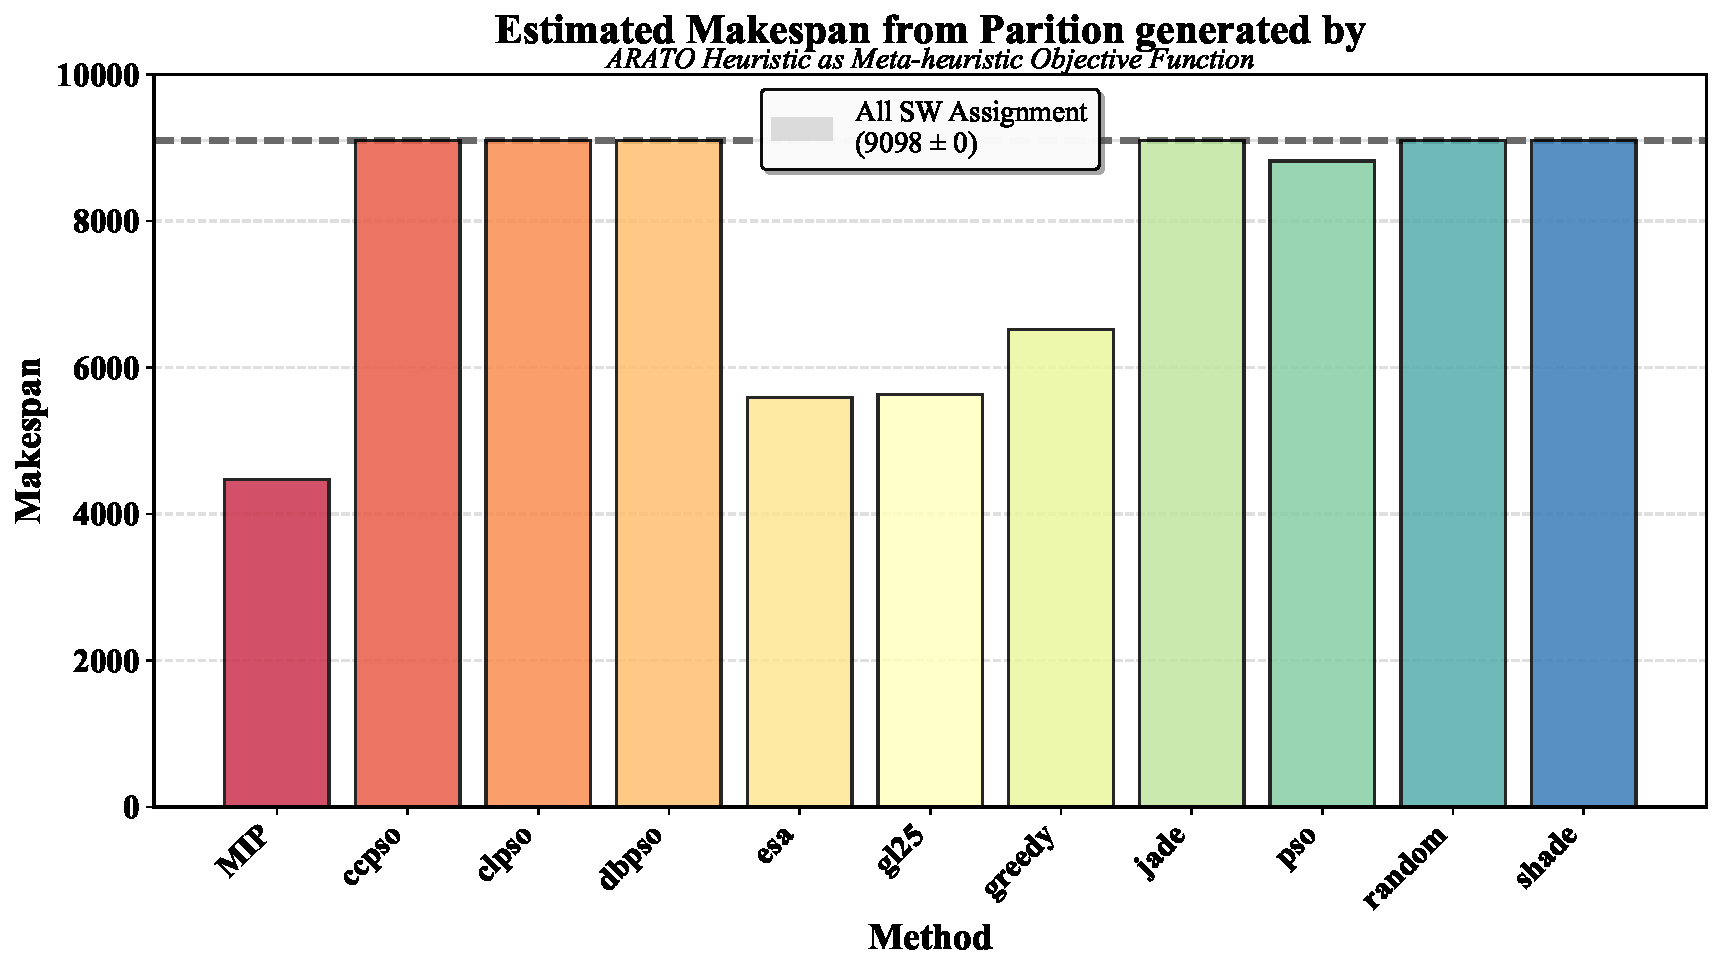
\includegraphics[width=0.48\linewidth]{Figures/meta-heuristic-Figures/arato-results-hw-0.1-area-0.5-seeds0-3-1.pdf}
    }
    \hfill
\subfloat[OPTM Heuristic\label{fig:optm_results}]{
        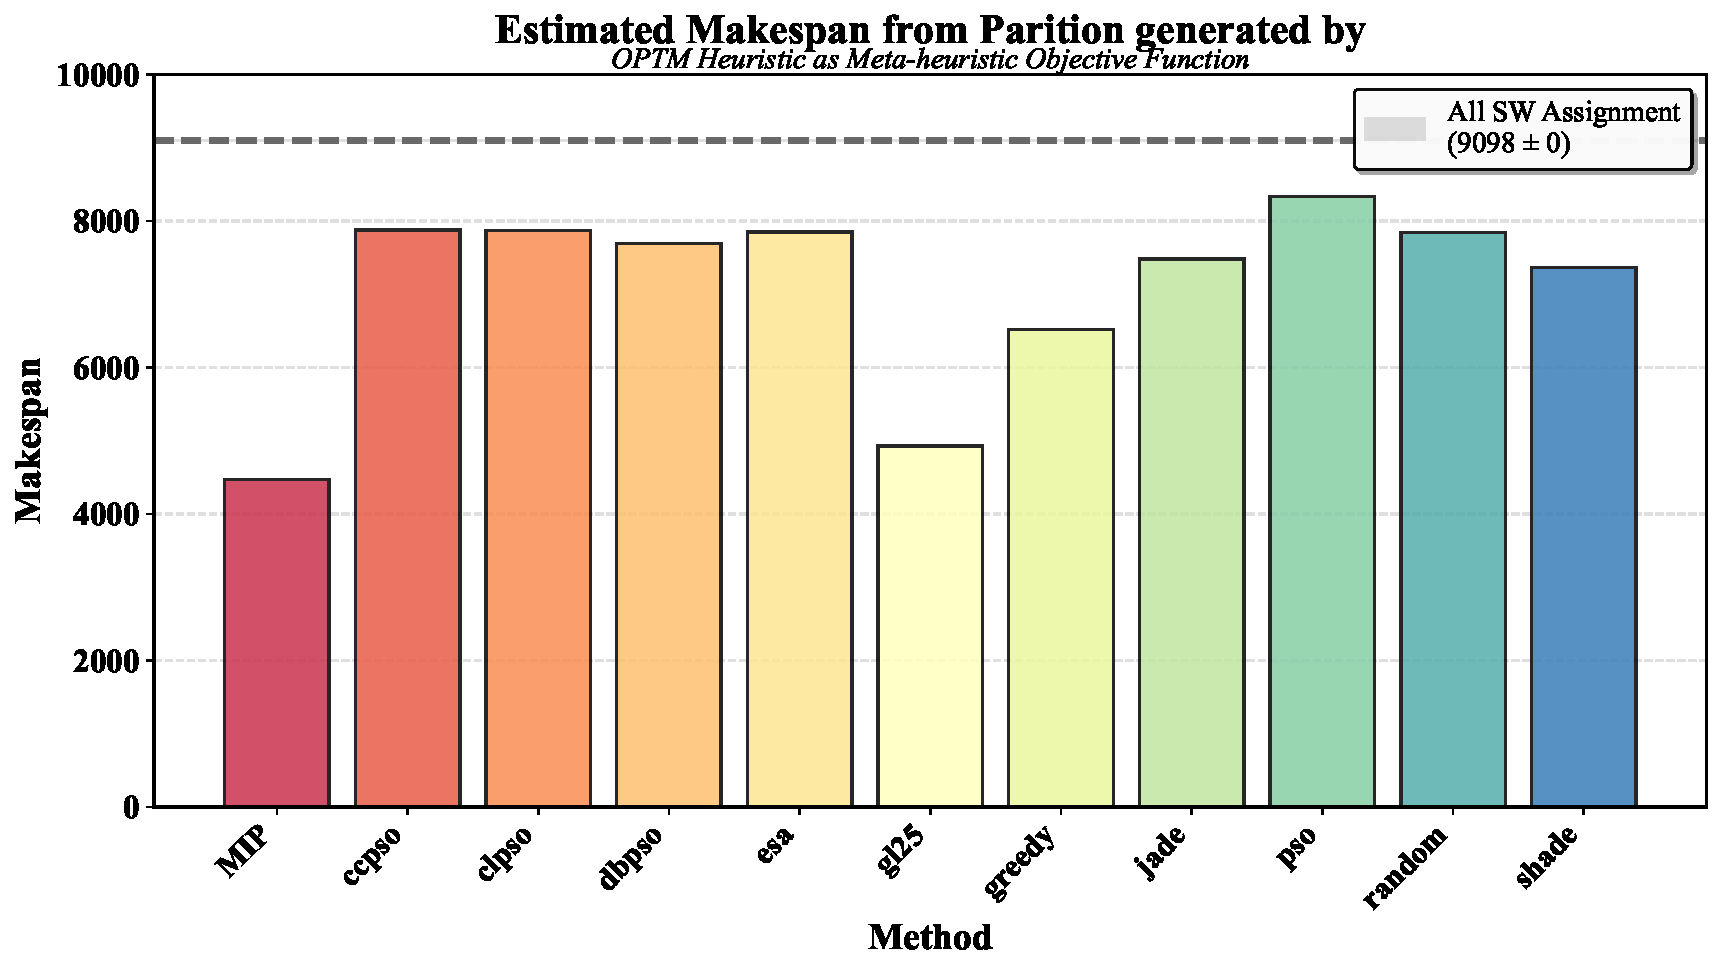
\includegraphics[width=0.48\linewidth]{Figures/meta-heuristic-Figures/makespan-results-hw-0.1-area-0.5-seeds0-3.pdf}
    }
    \hfill
    \subfloat[CA heuristic\label{fig:ca_results}]{
        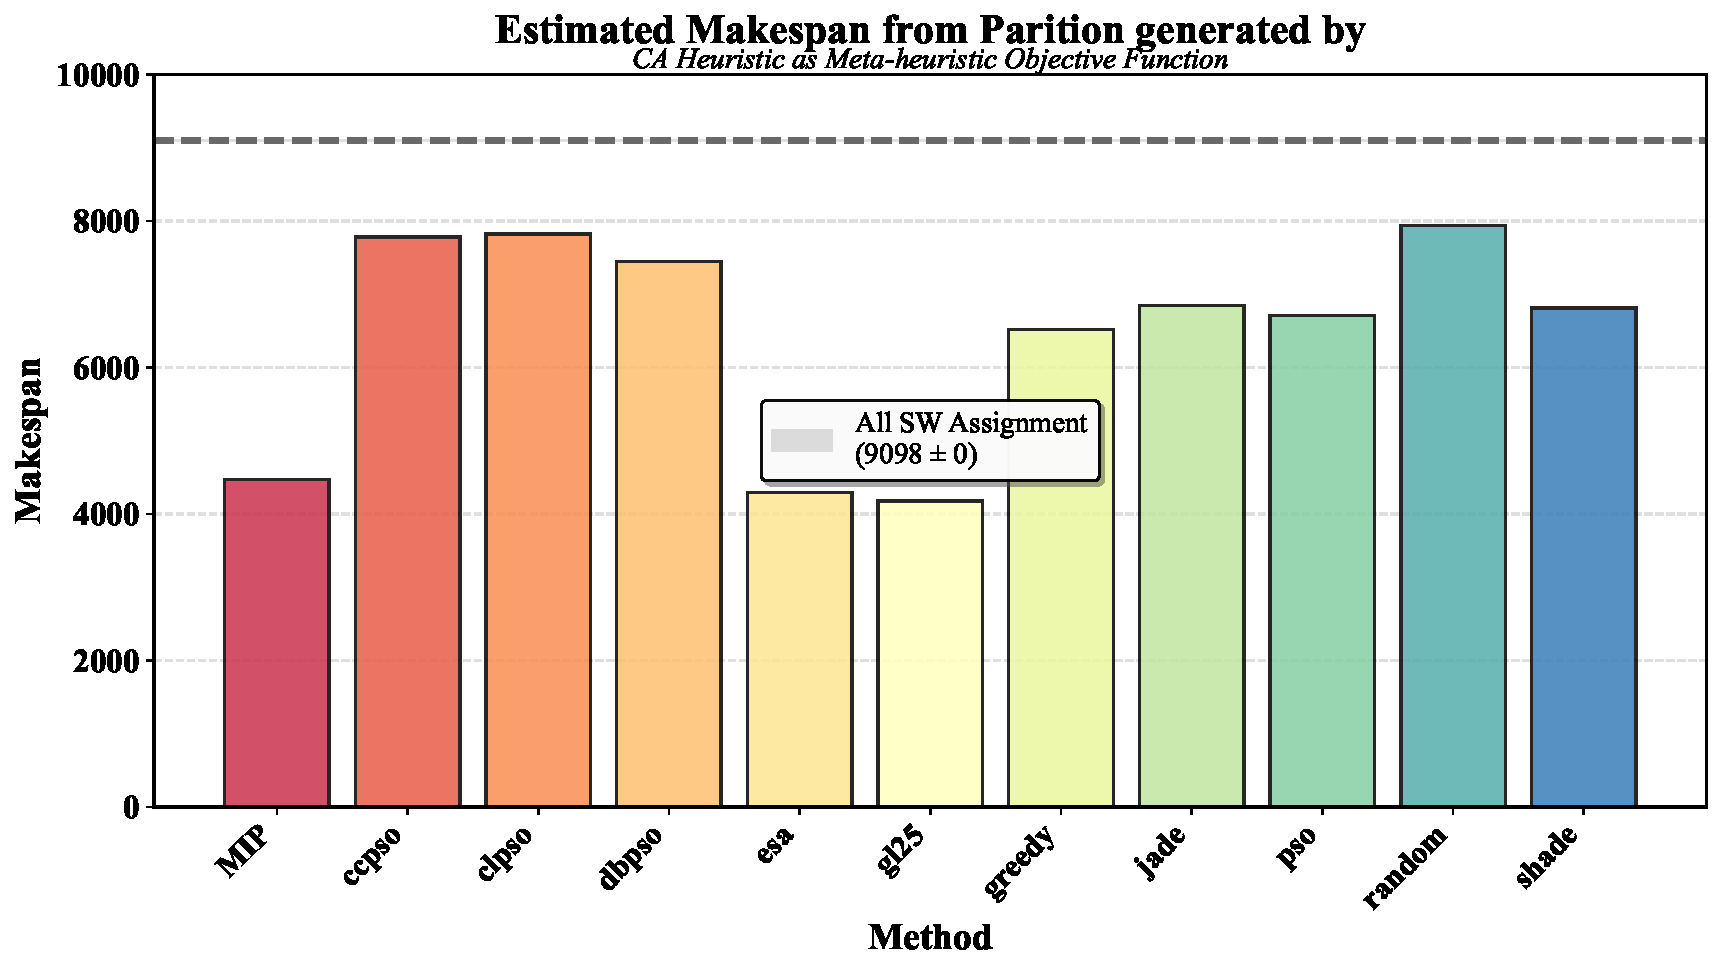
\includegraphics[width=0.48\linewidth]{Figures/meta-heuristic-Figures/comm-results-hw-0.1-area-0.5-seeds0-3.pdf}
    }
    \hfill
        \subfloat[CPL heuristic\label{fig:cpl_results}]{
        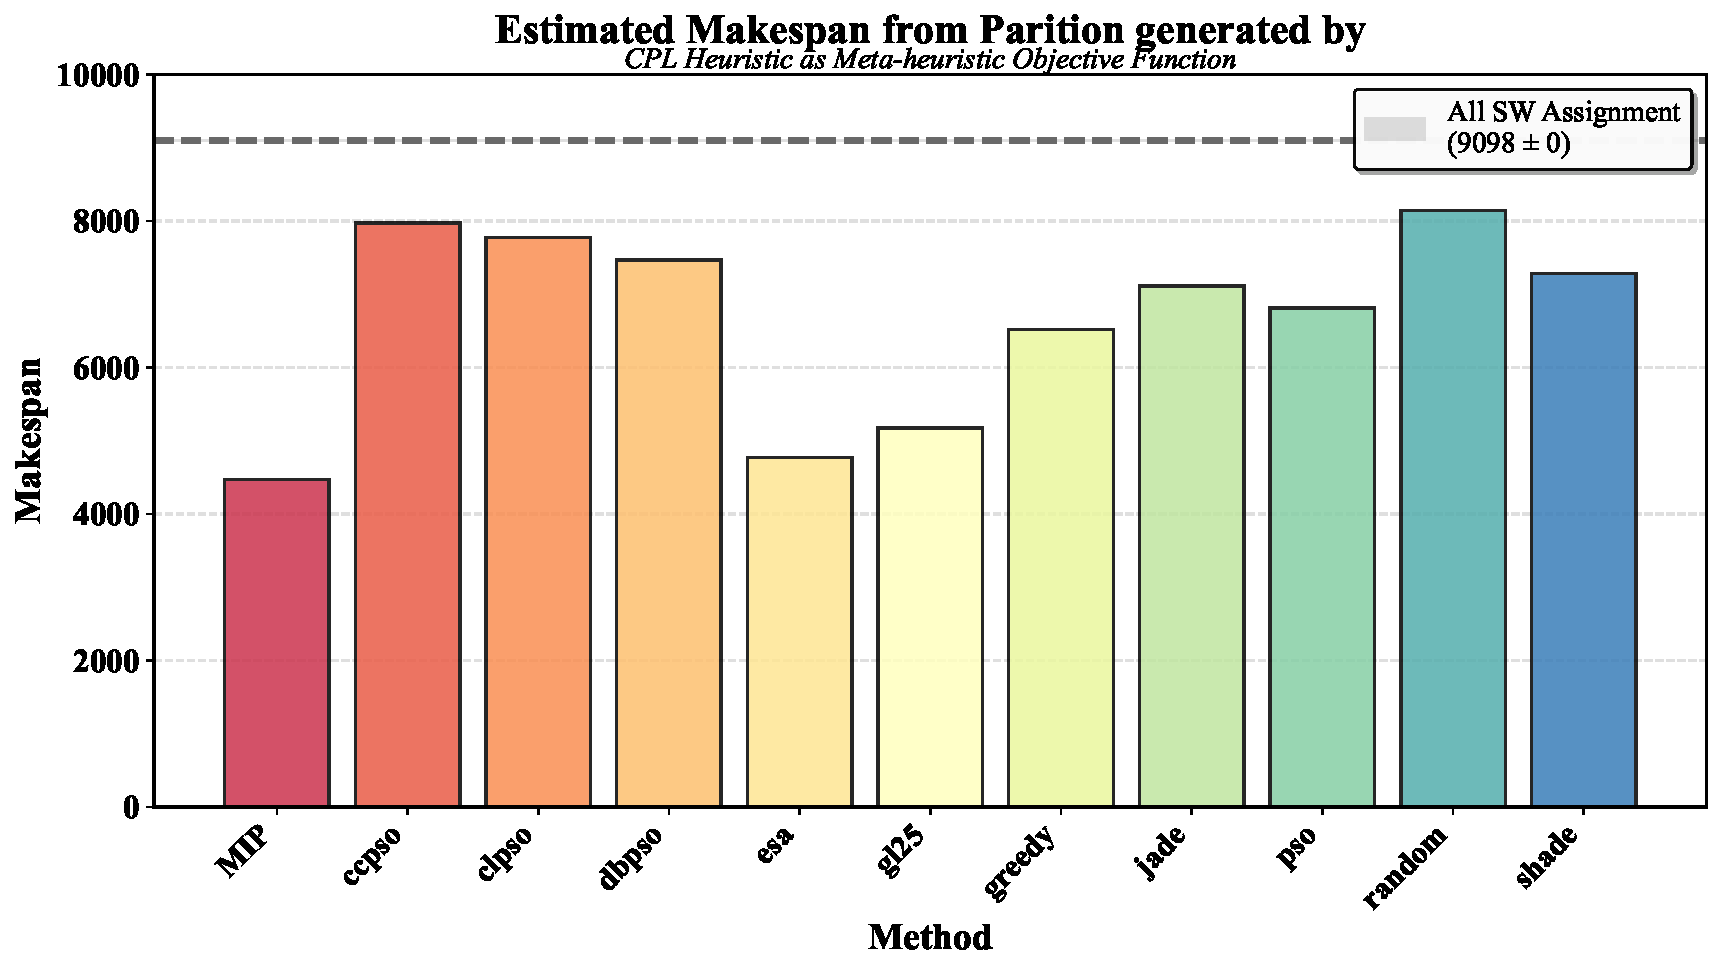
\includegraphics[width=0.48\linewidth]{Figures/meta-heuristic-Figures/cpl-results-hw-0.1-area-0.5-seeds0-3.pdf}
    }
    \hfill
        \subfloat[ED heuristic\label{fig:ed_results}]{
        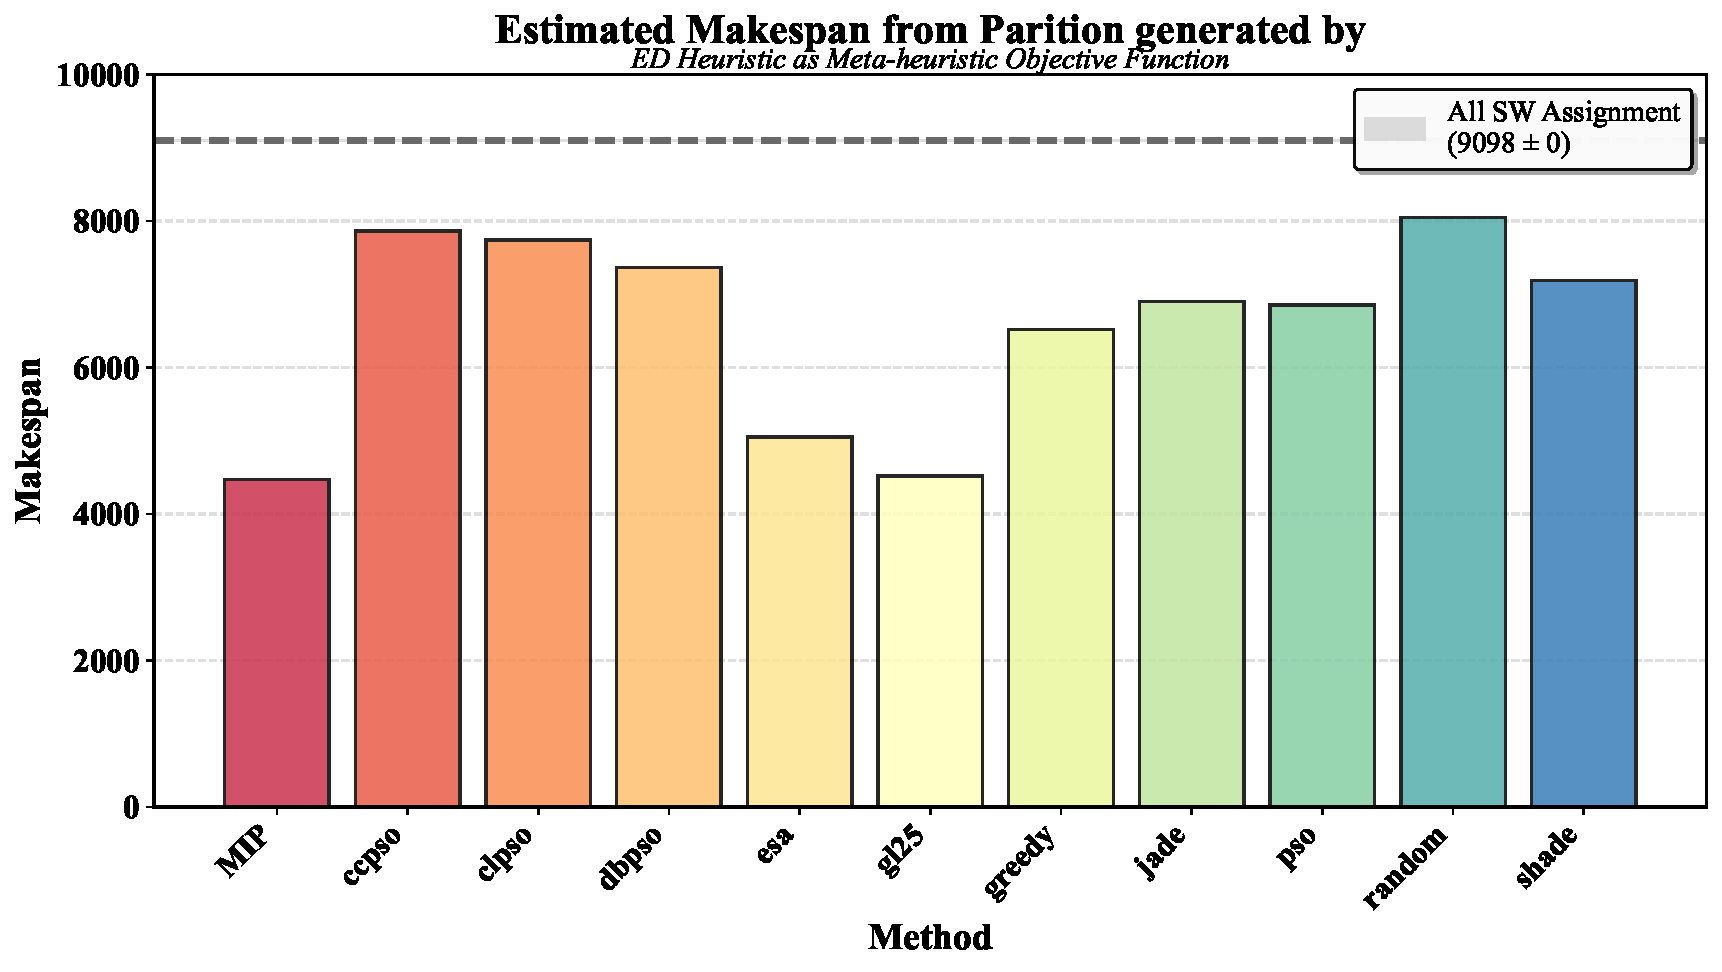
\includegraphics[width=0.48\linewidth]{Figures/meta-heuristic-Figures/ed-results-hw-0.1-area-0.5-seeds0-3.pdf}
    }
    \hfill
        \subfloat[SPT heuristic cost\label{fig:spt_results}]{
        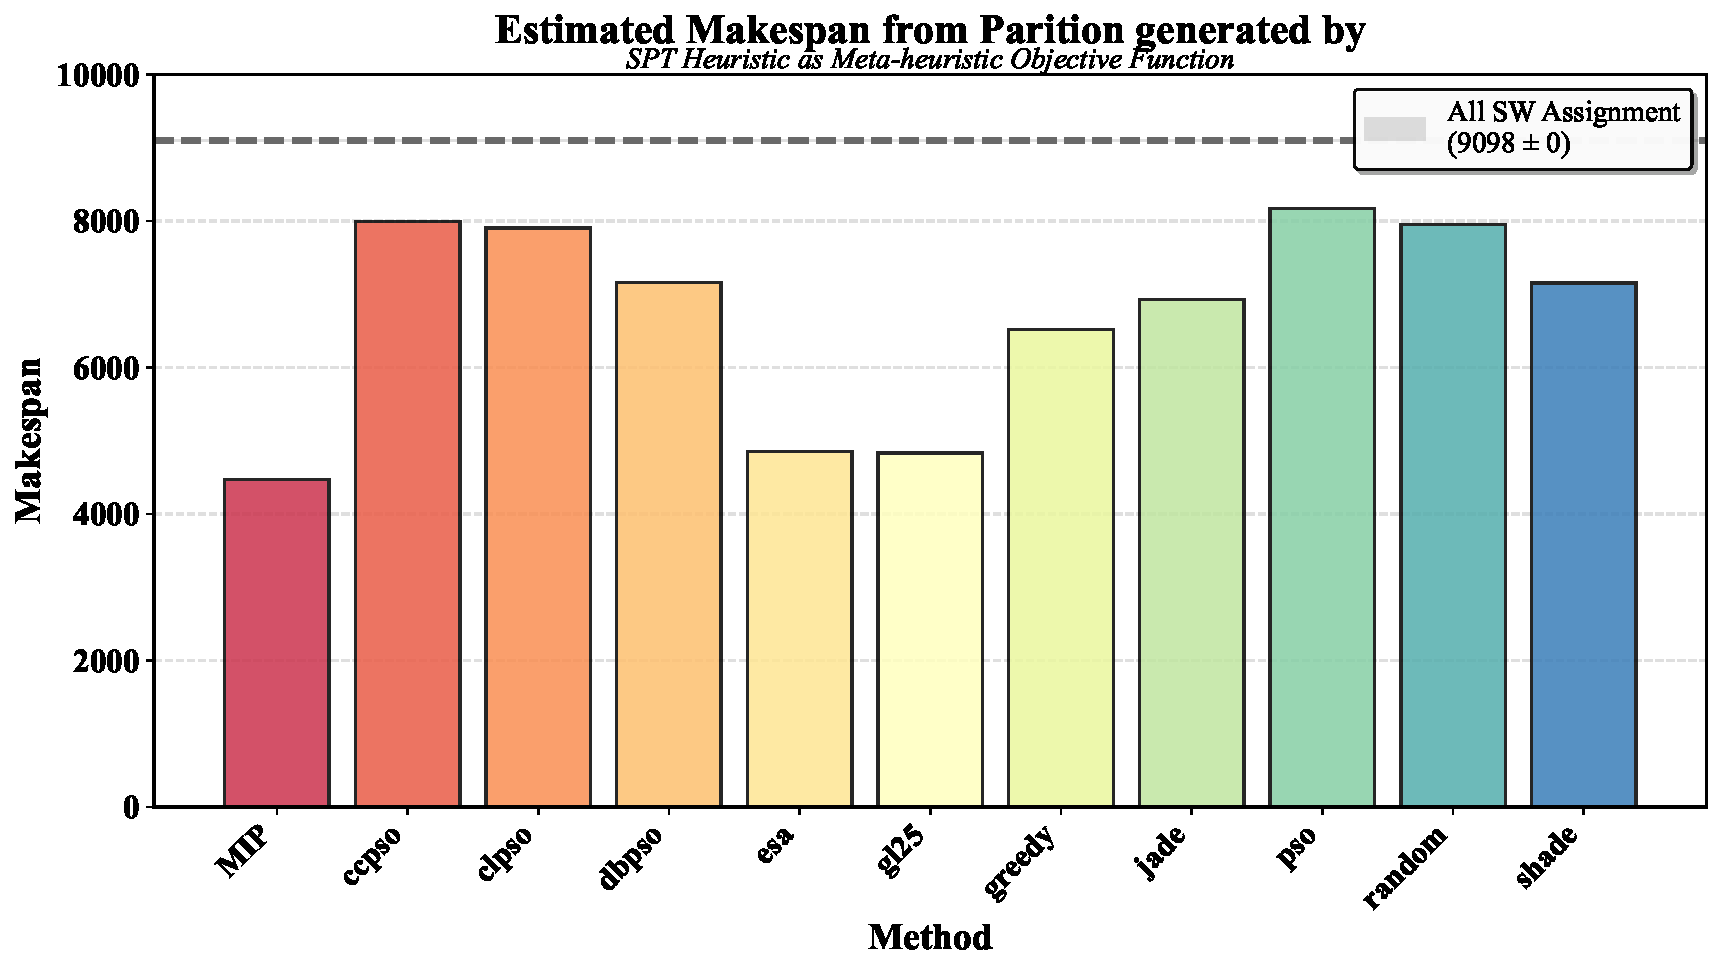
\includegraphics[width=0.48\linewidth]{Figures/meta-heuristic-Figures/spt-results-hw-0.1-area-0.5-seeds0-3.pdf}
    }
    \hfill

    \caption{{Comparison of Various Baseline MetaHeuristics on different optimization functions}}
    \label{fig:metaheur-compare}
    
\end{figure}

\begin{table}
\caption{\% Improvment of MIP over various meta heuristic methods for $k = 0.1, \alpha = 0.5$}
\begin{tabular}{llrrrrrrrr}
\toprule
 opt\_strategy & ccpso & clpso & dbpso & esa & gl25 & jade & pso & shade \\
\midrule
ARATO & 50.87 & 50.87 & 50.87 & 20.0 & 20.63 & 50.87 & 49.31 & 50.87 \\

CA & 42.55 & 42.83 & 40 & -4.16 & -7.05 & 34.68 & 33.38 & 34.37 \\

CPL & 43.94 & 42.5 & 40.14 & 6.35 & 13.55 & 37.18 & 34.39 & 38.6 \\

ED & 43.15 & 42.24 & 39.29 & 11.5 & 1.13 & 35.25 & 34.75 & 37.78 \\

OPTM & 43.27 & 43.21 & 41.91 & 43.05 & 9.35 & 40.27 & 46.38 & 39.29 \\

SPT & 44.09 & 43.44 & 37.56 & 7.94 & 7.56 & 35.45 & 45.30 & 37.45 \\
\bottomrule
\end{tabular}
\label{tab:mip_improvement}
\end{table}


\subsection{Results}

\subsubsection{SqueezeNet, $k=0.1, \alpha=0.5$}

Figure~\ref{fig:metaheur-compare} shows the performance of various methods with respect to various optimization strategies (Random and greedy does not have any).
Table~\ref{tab:mip_improvement} presents the percentage improvement of the Mixed Integer Programming (MIP) solution over various meta-heuristic methods for hardware scale factor $k = 0.1$ and area constraint $\alpha = 0.5$. The results reveal significant variations in performance across different optimization strategies and meta-heuristic algorithms.

\noindent
\textbf{Drawback of ARATO strategy}
The ARATO optimization strategy exhibits the poorest performance for the meta heuristics, with MIP outperforming most meta-heuristics by approximately 50\%, except for ESA (20.0\%) and GL25 (20.63\%). This substantial gap suggests that ARATO-based meta-heuristics struggle to find near-optimal solutions for the given problem constraints.

\noindent
\textbf{Best Performing Meta-Heuristics:}
Across all the optimization strategies, GL25 and ESA consistently demonstrate the smallest performance gaps relative to MIP. Notably, for the CA (Communication-Aware) strategy, both methods achieve superior evaluation metrics compared to MIP. \zmcomment{This is due to MIP jointly solving partitioning and scheduling, and the evaluation function takes a specific scheduling. Thus, the superiority of the MIP may be overlooked here}. This suggests that for communication-intensive objectives, meta-heuristics can explore solution spaces more effectively than exact methods within practical time constraints. --\zmcomment{May not be necessarily true, but given the current nature of evaluation, this is the best I can put}

\noindent
\textbf{Strategy-Specific Observations:}
\begin{itemize}
    \item \textbf{ARATO:} Shows poor performance across PSO variants (PSO, DBPSO, CCPSO, CLPSO, JADE, SHADE), suggesting these methods converge to similar suboptimal regions for this strategy.
    
    \item \textbf{CA (Communication-Aware):} Exhibits the most varied performance, with GL25 and ESA achieving superior solutions to MIP while PSO variants lag by 33--43\%. This indicates that genetic algorithms and simulated annealing better capture the communication cost structure.
    
    \item \textbf{OPTM (Makespan Optimization):} PSO has the largest improvement gap (46.38\%), while GL25 shows exceptional performance with only 9.35\% gap, demonstrating the effectiveness of genetic approaches for scheduling-oriented objectives.
    
    \item \textbf{CPL, ED, and SPT:} These strategies show similar margins, with GL25 and ESA consistently performing better than PSO-based approaches.
\end{itemize}

\textbf{Algorithm Family Comparison:}
\begin{itemize}
    \item \textit{PSO Variants} (PSO, DBPSO, CCPSO, CLPSO): Demonstrate relatively consistent performance within each strategy, with optimality gaps ranging from 33--50\%. CCPSO and CLPSO variations show minimal differentiation from standard PSO.
    
    \item \textit{Differential Evolution} (JADE, SHADE): Perform comparably to PSO variants, with JADE generally achieving slightly better results than SHADE across most strategies.
    
    \item \textit{Genetic Algorithm} (GL25): Stands out as the most competitive meta-heuristic, achieving the smallest gaps across five of six strategies.
    
    \item \textit{Simulated Annealing} (ESA): Shows strong performance particularly in CA and CPL strategies.
\end{itemize}

% Figure~\ref{fig:makespan_results} and Figure~\ref{fig:partition_cost_results} present the comparative performance of all implemented meta-heuristic methods across both objective functions. The results reveal significant performance variations among different algorithmic approaches, with clear distinctions between the effectiveness of various optimization paradigms.

% For makespan minimization, GL25 emerges as the most effective method, achieving an estimated makespan of approximately 4,700 time units, representing a substantial improvement over the all-software baseline of 8,500 units. This corresponds to a makespan reduction of approximately 45\%, demonstrating the significant potential of hardware-software co-design optimization. CLPSO and SHADE also demonstrate competitive performance, achieving makespans around 7,800 time units, while other methods including DBPSO, Random, PSO, JADE, CCPSO, and Greedy cluster around 8,000 time units, showing marginal improvements over the naive all-software assignment. Notably, ESA achieves a makespan of approximately 7,500 units, positioning it in the middle tier of performance.

% In terms of partition cost optimization, the results show a different performance ranking. GL25 again demonstrates superior performance with the lowest partition cost of approximately 7,400 units, significantly outperforming all other methods. CLPSO, SHADE, and ESA achieve competitive results with partition costs ranging from 7,400 to 8,600 units, all maintaining costs below the all-software baseline. Interestingly, the Greedy heuristic produces the highest partition cost at approximately 12,500 units, suggesting that the simple gain-per-area ratio approach may not be optimal for this particular problem configuration. The remaining methods (DBPSO, Random, PSO, JADE, CCPSO) exhibit similar performance levels, clustering around 8,400-8,700 units.

Our first analysis reveals that GL25 and ESA consistently achieve superior performance across all objective functions, establishing it as the most robust methods for this particular task graph configuration.
\zmcomment{Note that ESA,GL25 have higher iterations than many other (except SHADE, JADE)}

\zmcomment{Before proceeding more, we need to decide the following.

\begin{enumerate}
    \item All experimental configurations -- number of environment parameters to evaluate against, how many run per each config.

    \item task graphs -- how many taskgraphs to evaluate against

    \item evaluation functions -- what function to use for evaluation

\end{enumerate}
}




% \section{Sensitivity Analysis}


\begin{figure*}[]  % Use [p] for a dedicated page
\centering
\caption{Sensitivity analysis of meta-heuristic performance across optimization strategies, hardware scale factors and area constraint}
\label{fig:sensitivity_all}

% Row 1: ARATO
\subfloat[ARATO, $k=0.1$]{%
    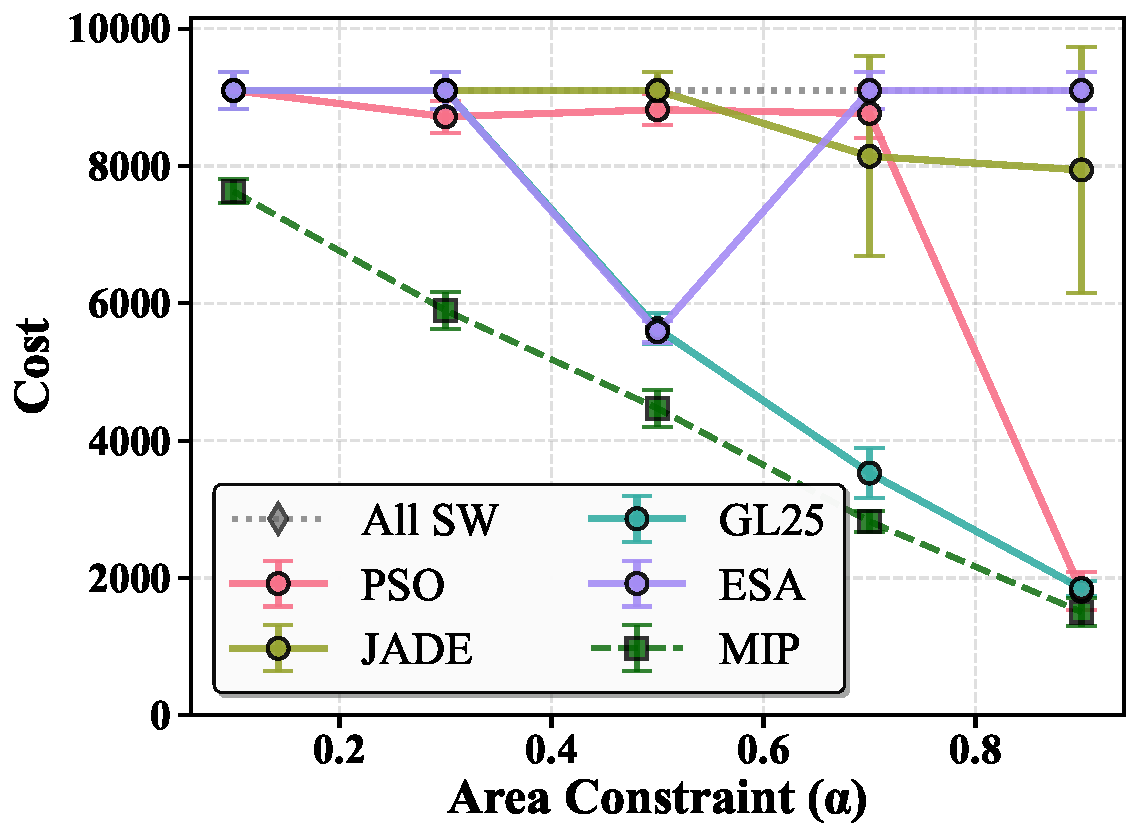
\includegraphics[width=0.32\textwidth]{Figures/meta-heuristic-Figures/sensitivity_methods_vs_area_hw_0.1_strategy_ARATO.pdf}
}\hfill
\subfloat[ARATO, $k=0.5$]{%
    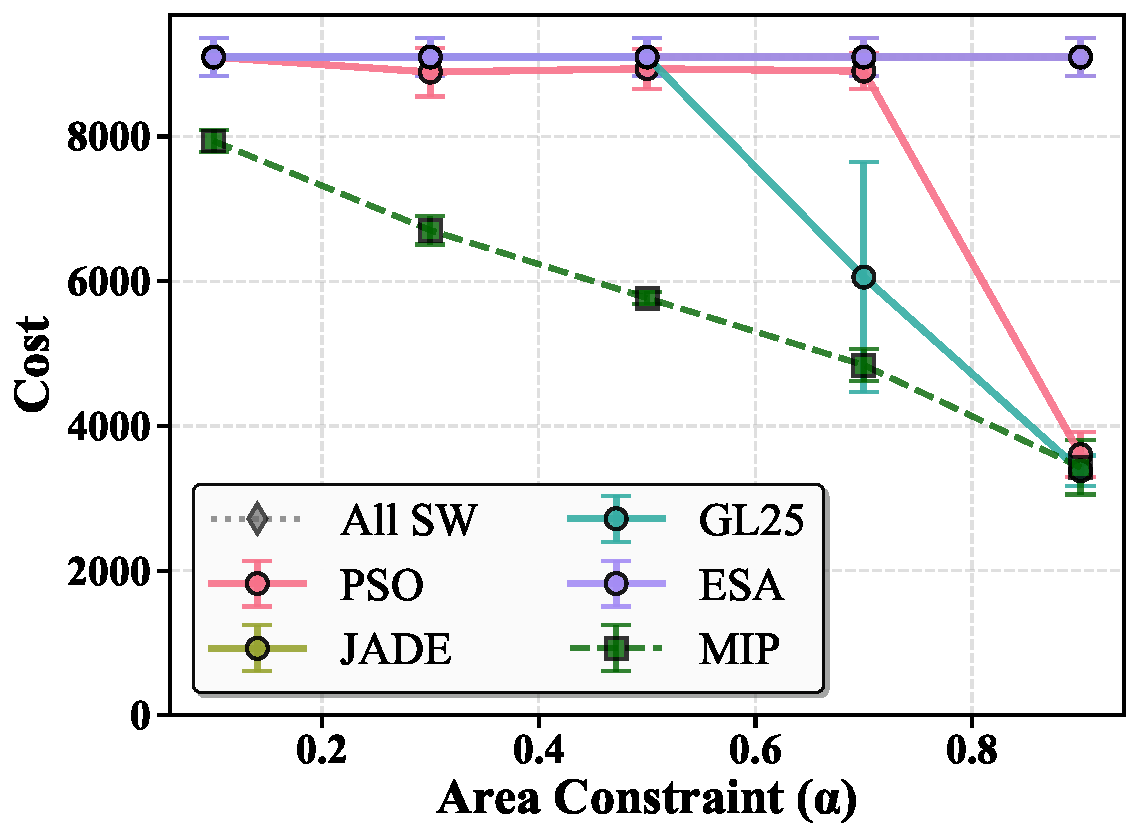
\includegraphics[width=0.32\textwidth]{Figures/meta-heuristic-Figures/sensitivity_methods_vs_area_hw_0.5_strategy_ARATO.pdf}
}\hfill
\subfloat[ARATO, $k=0.9$]{%
    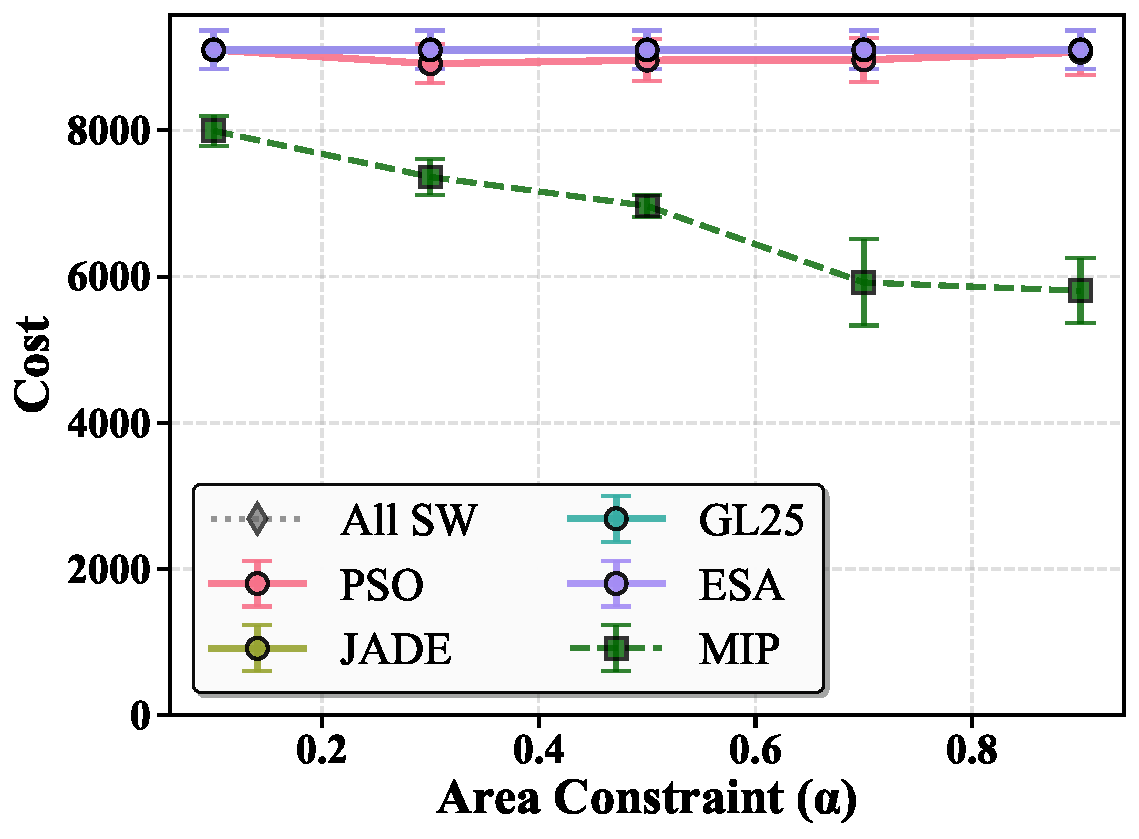
\includegraphics[width=0.32\textwidth]{Figures/meta-heuristic-Figures/sensitivity_methods_vs_area_hw_0.9_strategy_ARATO.pdf}
}\\

% Row 2: CA
\subfloat[CA, $k=0.1$]{%
    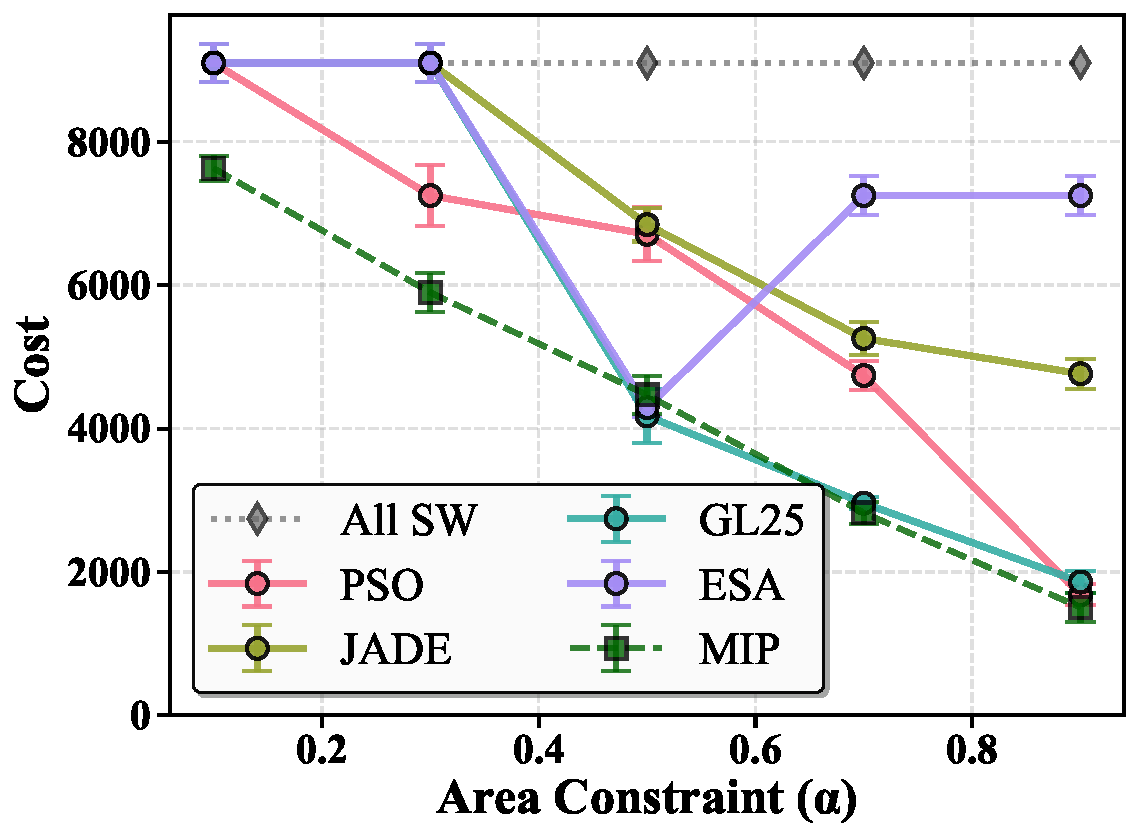
\includegraphics[width=0.32\textwidth]{Figures/meta-heuristic-Figures/sensitivity_methods_vs_area_hw_0.1_strategy_CA.pdf}
}\hfill
\subfloat[CA, $k=0.5$]{%
    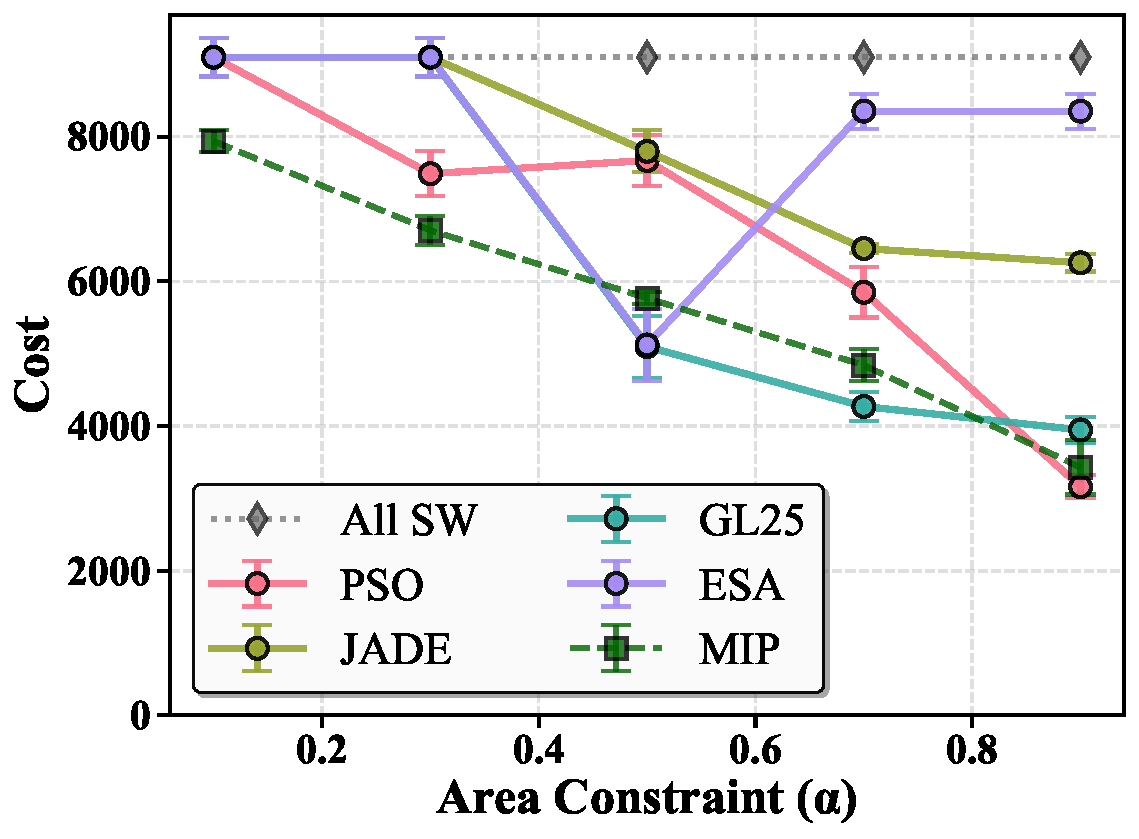
\includegraphics[width=0.32\textwidth]{Figures/meta-heuristic-Figures/sensitivity_methods_vs_area_hw_0.5_strategy_CA.pdf}
}\hfill
\subfloat[CA, $k=0.9$]{%
    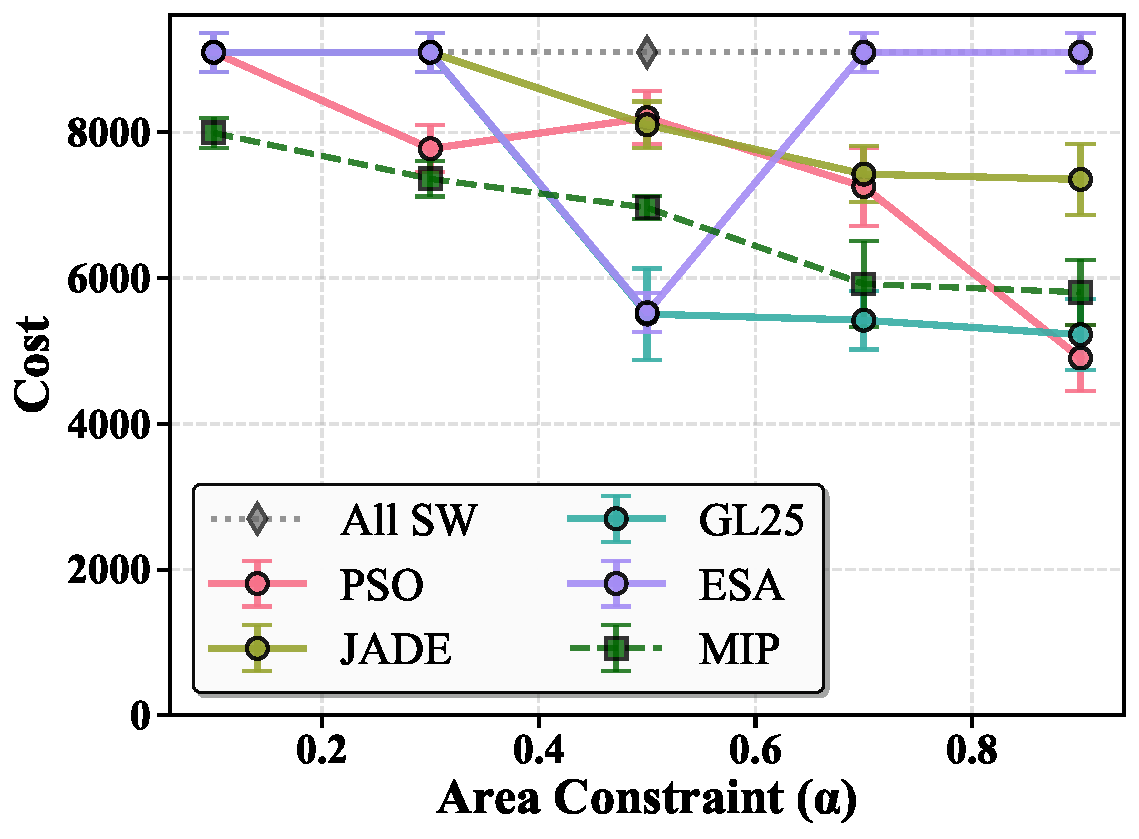
\includegraphics[width=0.32\textwidth]{Figures/meta-heuristic-Figures/sensitivity_methods_vs_area_hw_0.9_strategy_CA.pdf}
}\\

% Row 3: CPL
% \subfloat[CPL, $k=0.1$]{%
%     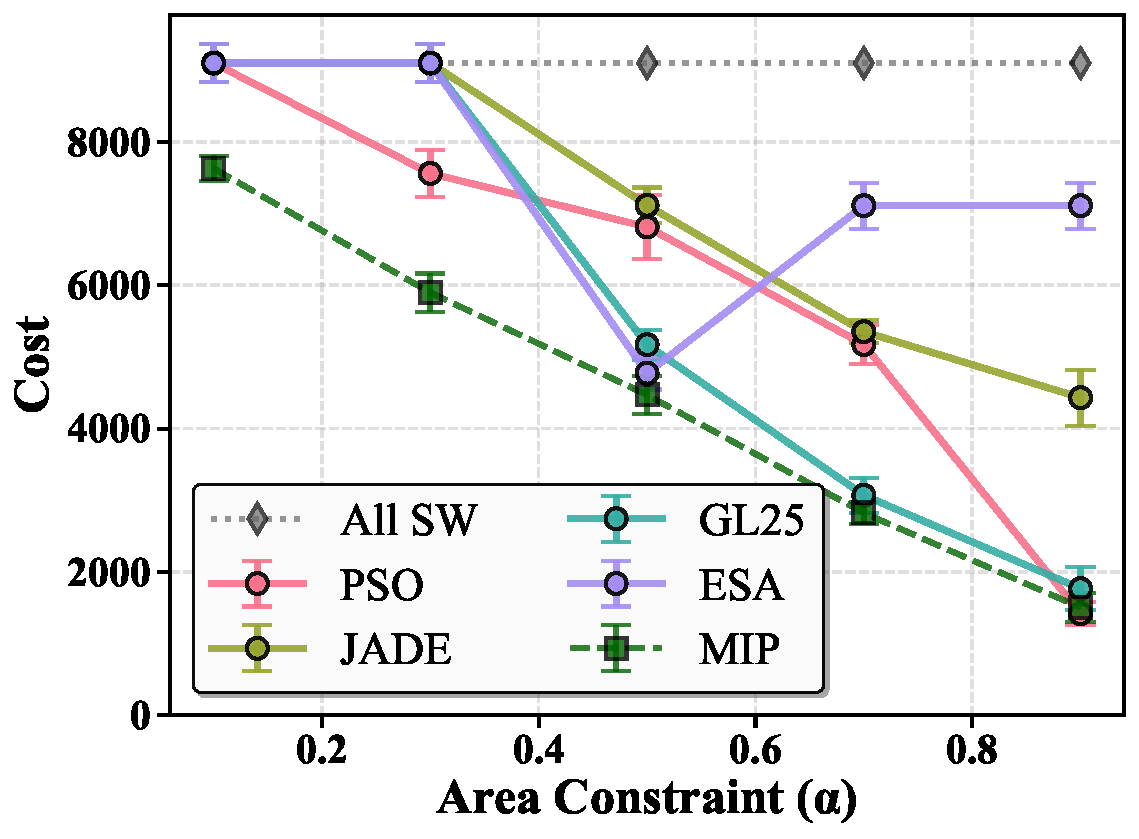
\includegraphics[width=0.32\textwidth]{Figures/meta-heuristic-Figures/sensitivity_methods_vs_area_hw_0.1_strategy_CPL.pdf}
% }\hfill
% \subfloat[CPL, $k=0.5$]{%
%     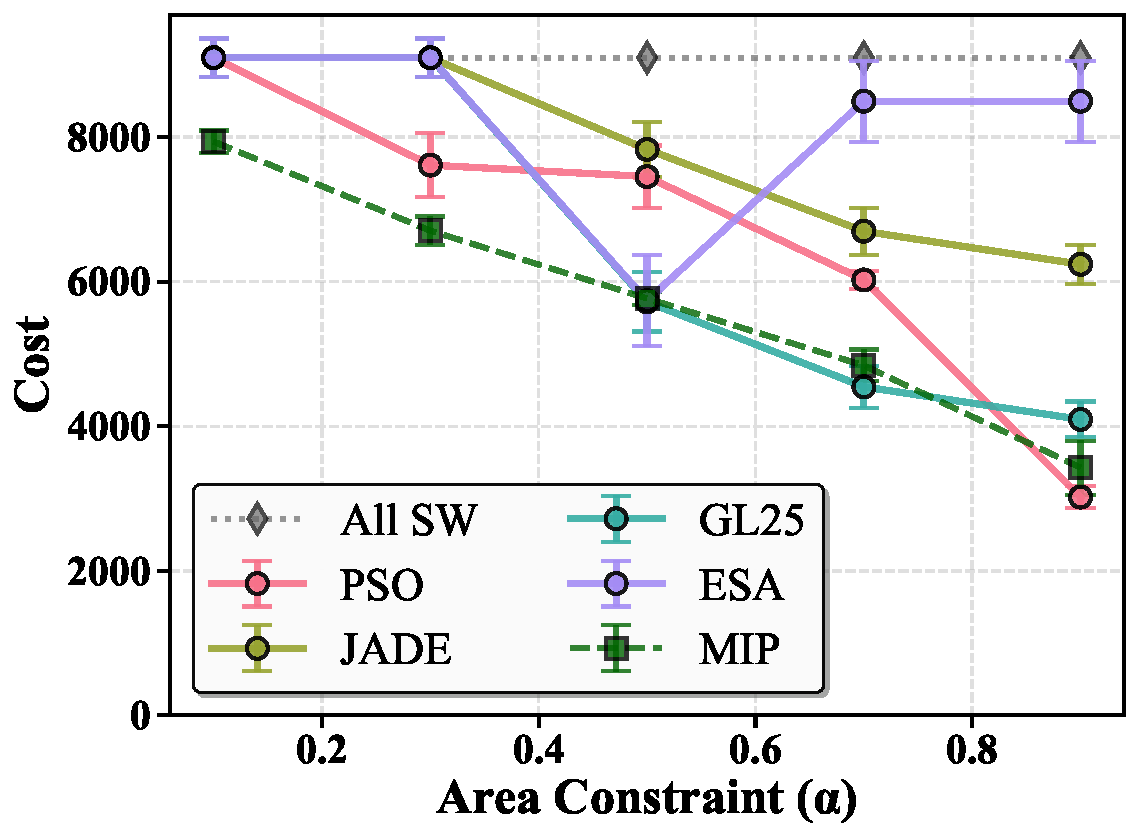
\includegraphics[width=0.32\textwidth]{Figures/meta-heuristic-Figures/sensitivity_methods_vs_area_hw_0.5_strategy_CPL.pdf}
% }\hfill
% \subfloat[CPL, $k=0.9$]{%
%     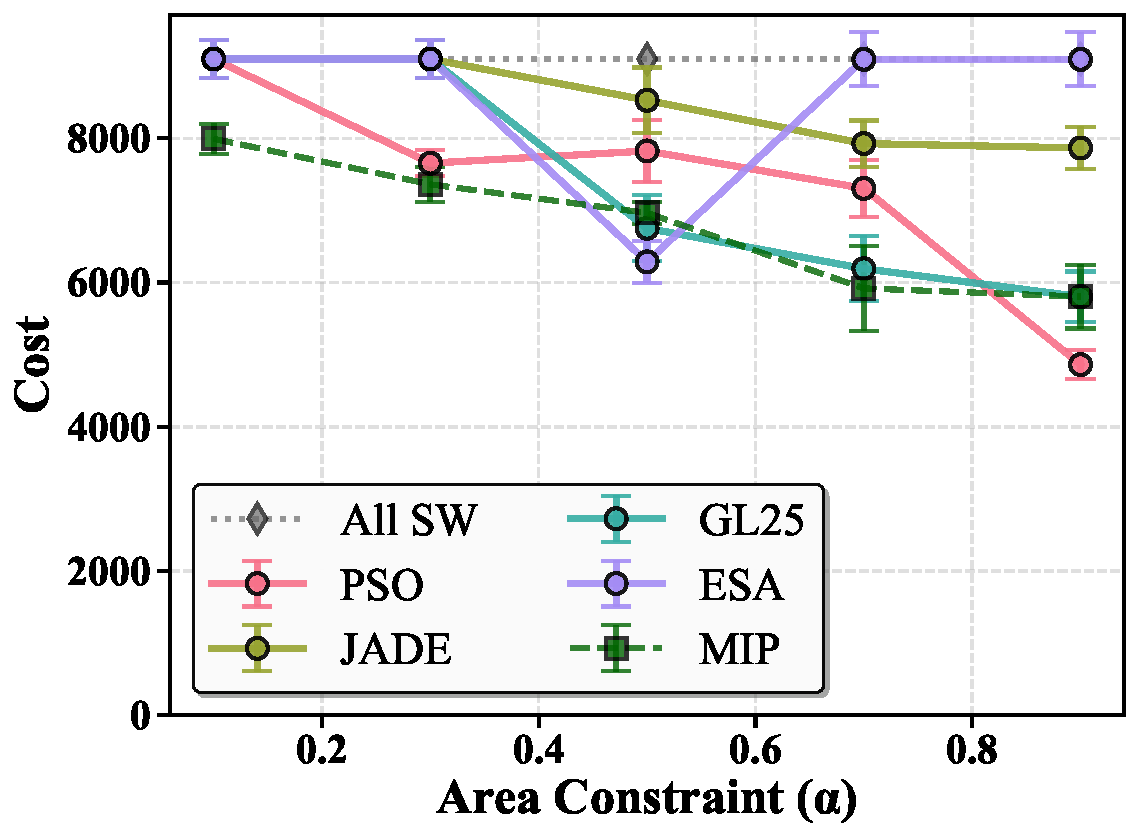
\includegraphics[width=0.32\textwidth]{Figures/meta-heuristic-Figures/sensitivity_methods_vs_area_hw_0.9_strategy_CPL.pdf}
% }\\

% % Row 4: ED
% \subfloat[ED, $k=0.1$]{%
%     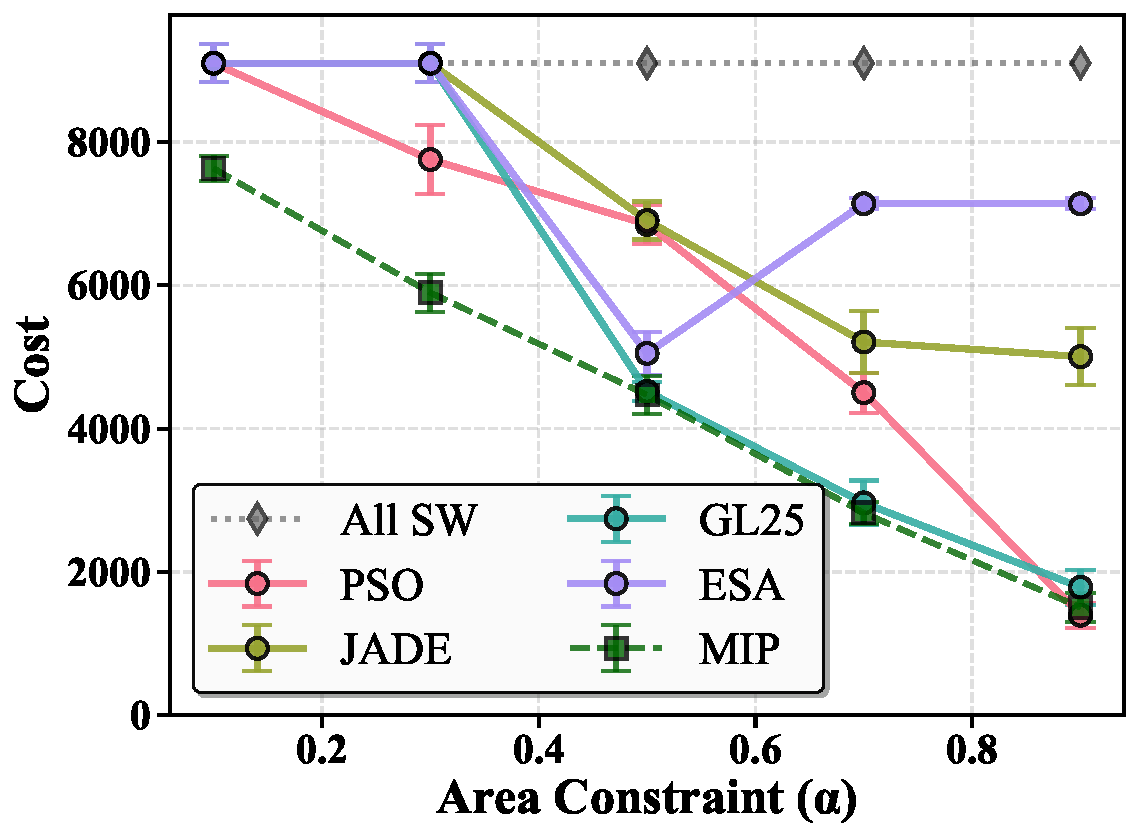
\includegraphics[width=0.32\textwidth]{Figures/meta-heuristic-Figures/sensitivity_methods_vs_area_hw_0.1_strategy_ED.pdf}
% }\hfill
% \subfloat[ED, $k=0.5$]{%
%     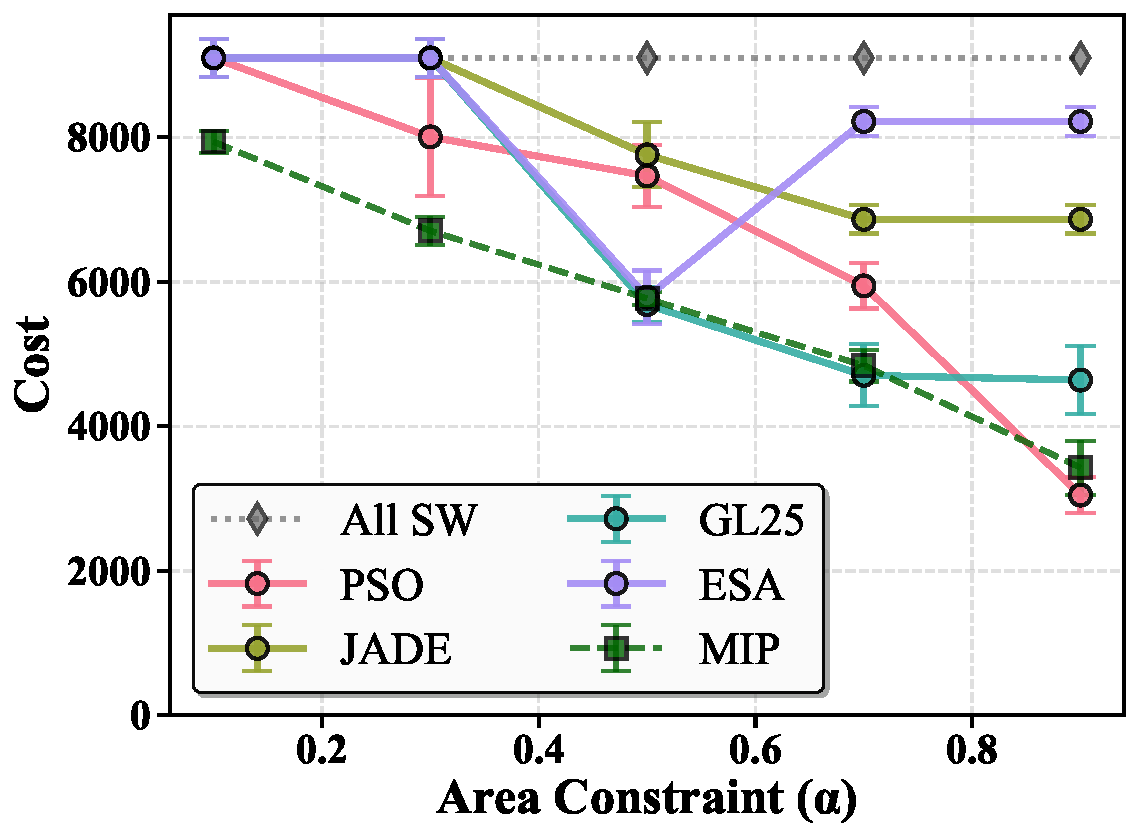
\includegraphics[width=0.32\textwidth]{Figures/meta-heuristic-Figures/sensitivity_methods_vs_area_hw_0.5_strategy_ED.pdf}
% }\hfill
% \subfloat[ED, $k=0.9$]{%
%     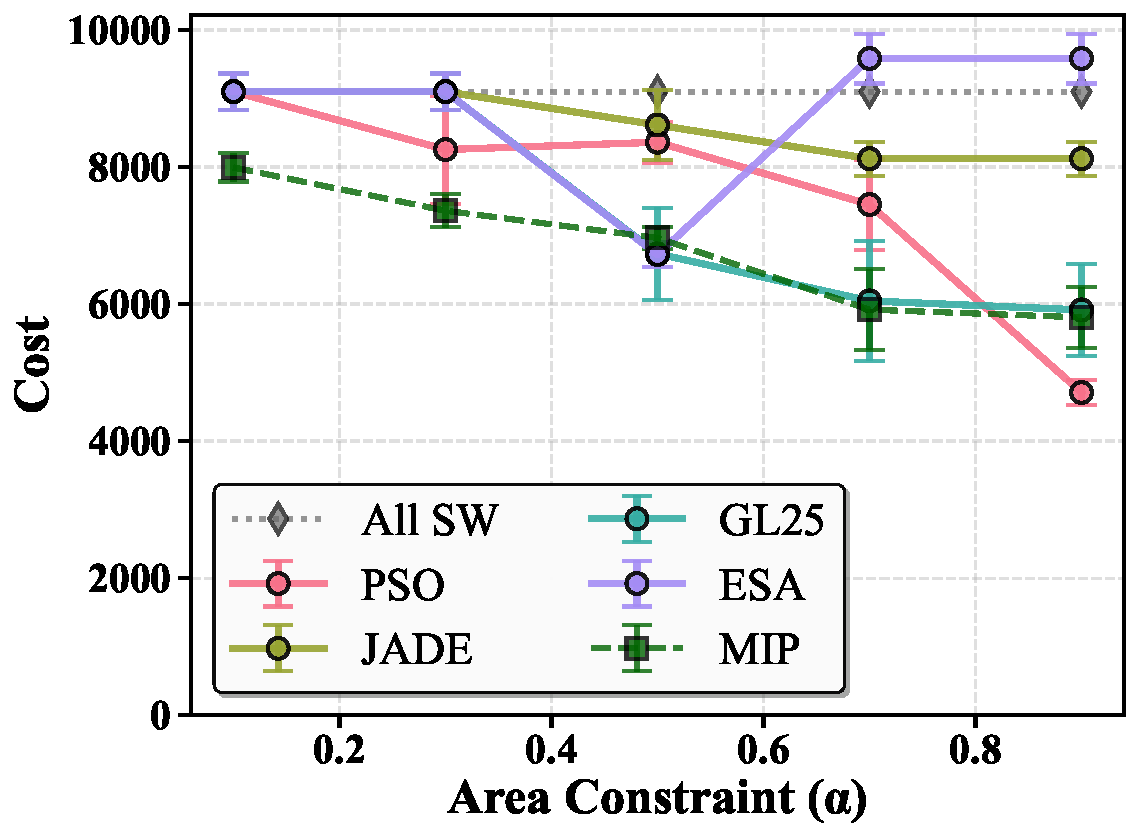
\includegraphics[width=0.32\textwidth]{Figures/meta-heuristic-Figures/sensitivity_methods_vs_area_hw_0.9_strategy_ED.pdf}
% }\\

% % Row 5: SPT
% \subfloat[SPT, $k=0.1$]{%
%     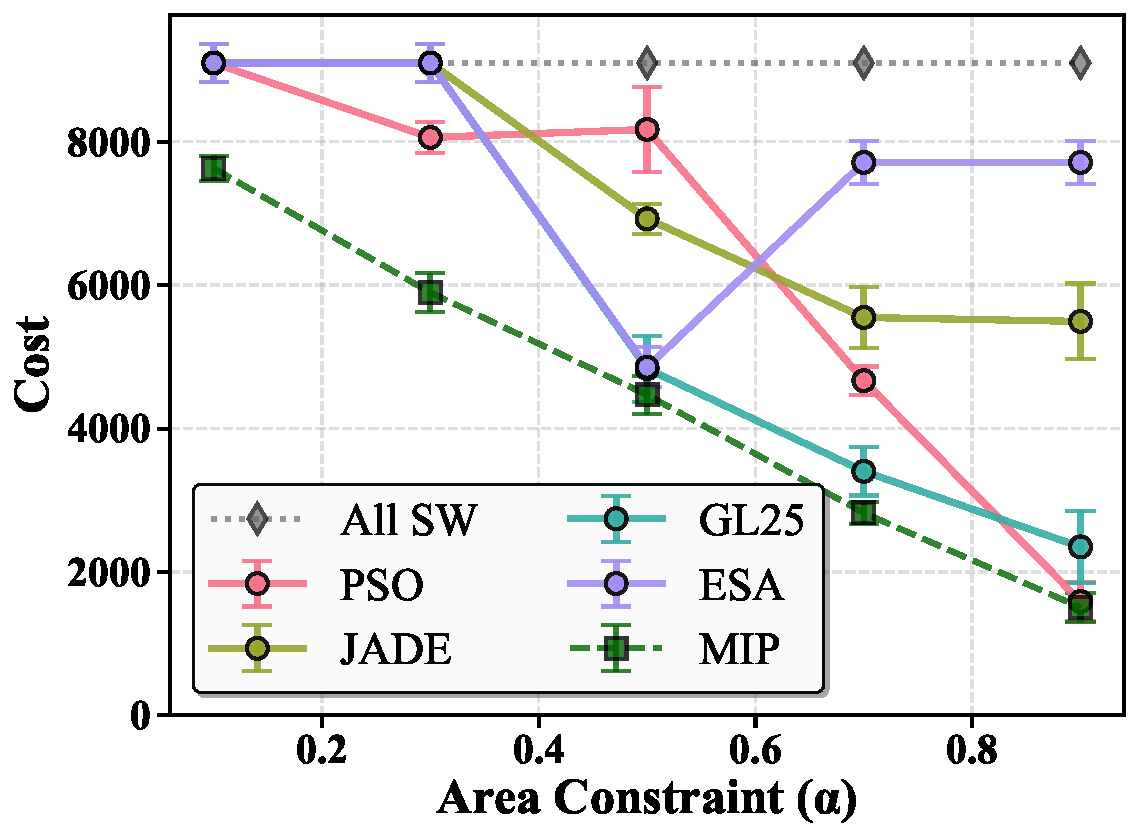
\includegraphics[width=0.32\textwidth]{Figures/meta-heuristic-Figures/sensitivity_methods_vs_area_hw_0.1_strategy_SPT.pdf}
% }\hfill
% \subfloat[SPT, $k=0.5$]{%
%     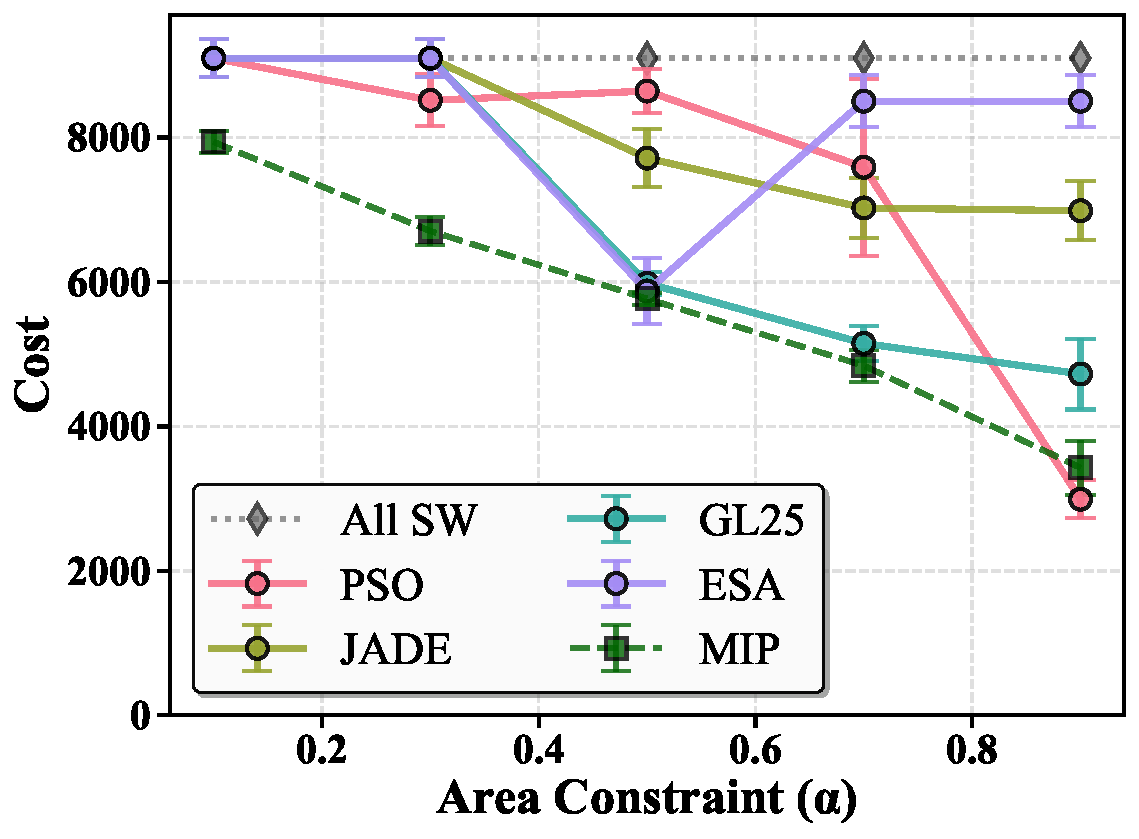
\includegraphics[width=0.32\textwidth]{Figures/meta-heuristic-Figures/sensitivity_methods_vs_area_hw_0.5_strategy_SPT.pdf}
% }\hfill
% \subfloat[SPT, $k=0.9$]{%
%     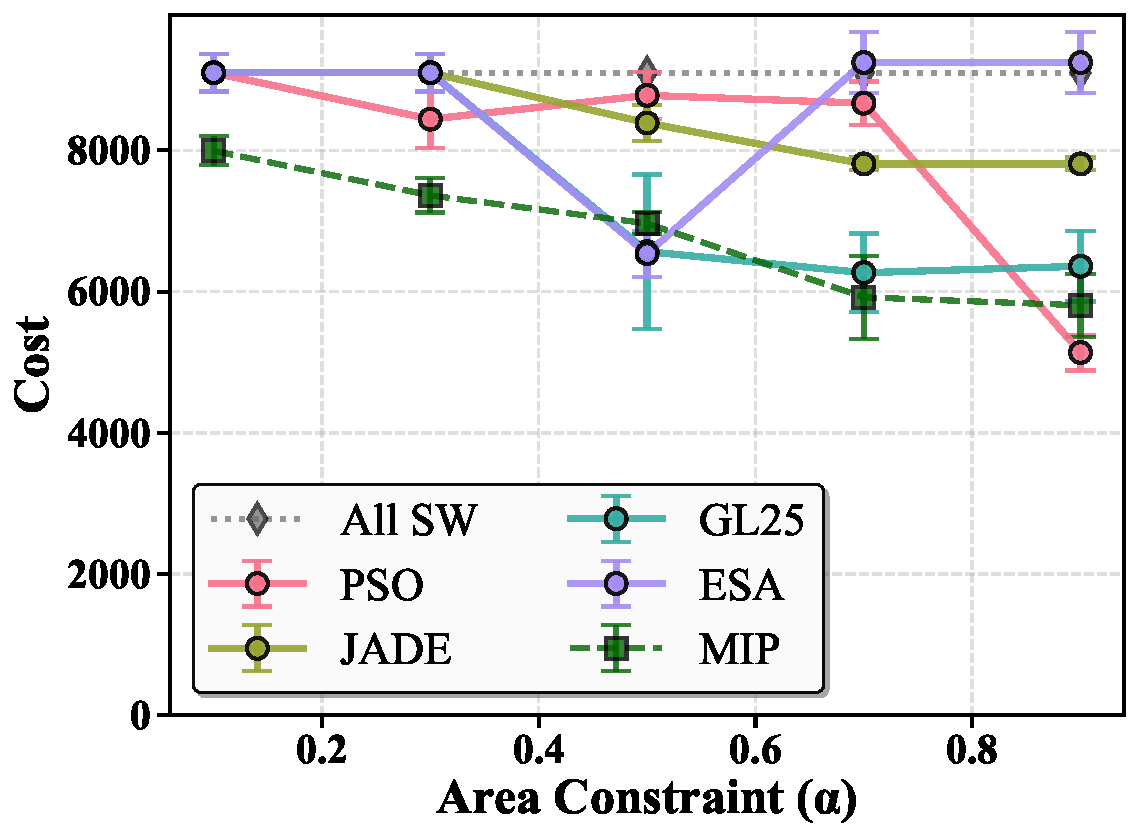
\includegraphics[width=0.32\textwidth]{Figures/meta-heuristic-Figures/sensitivity_methods_vs_area_hw_0.9_strategy_SPT.pdf}
% }\\

% Row 6: OPTM
% \subfloat[OPTM, $k=0.1$]{%
%     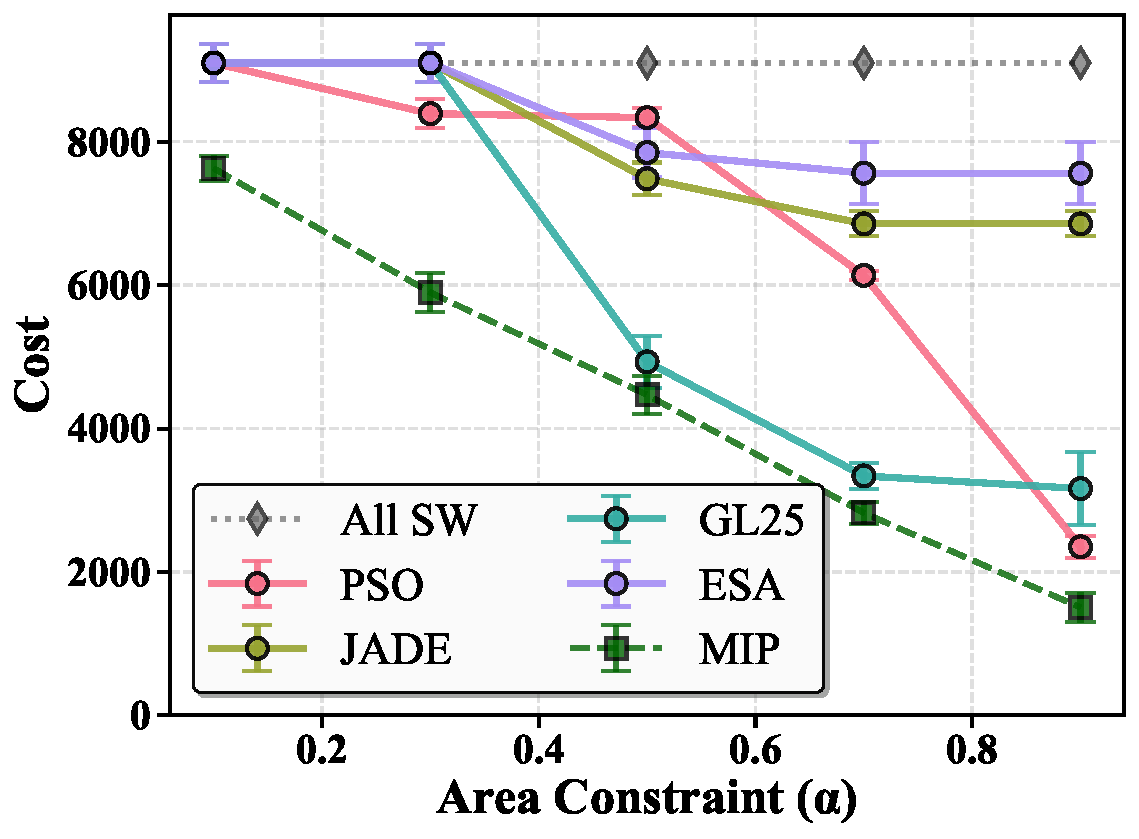
\includegraphics[width=0.32\textwidth]{Figures/meta-heuristic-Figures/sensitivity_methods_vs_area_hw_0.1_strategy_OPTM.pdf}
% }\hfill
% \subfloat[OPTM, $k=0.5$]{%
%     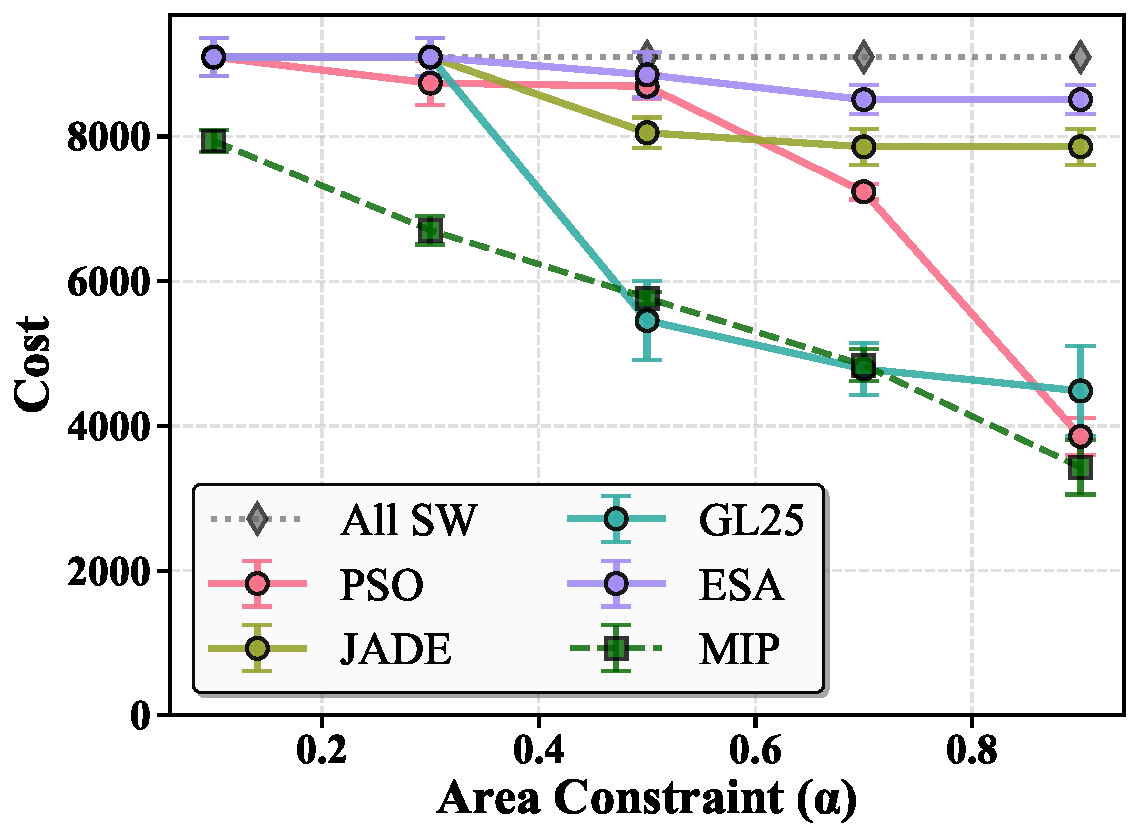
\includegraphics[width=0.32\textwidth]{Figures/meta-heuristic-Figures/sensitivity_methods_vs_area_hw_0.5_strategy_OPTM.pdf}
% }\hfill
% \subfloat[OPTM, $k=0.9$]{%
%     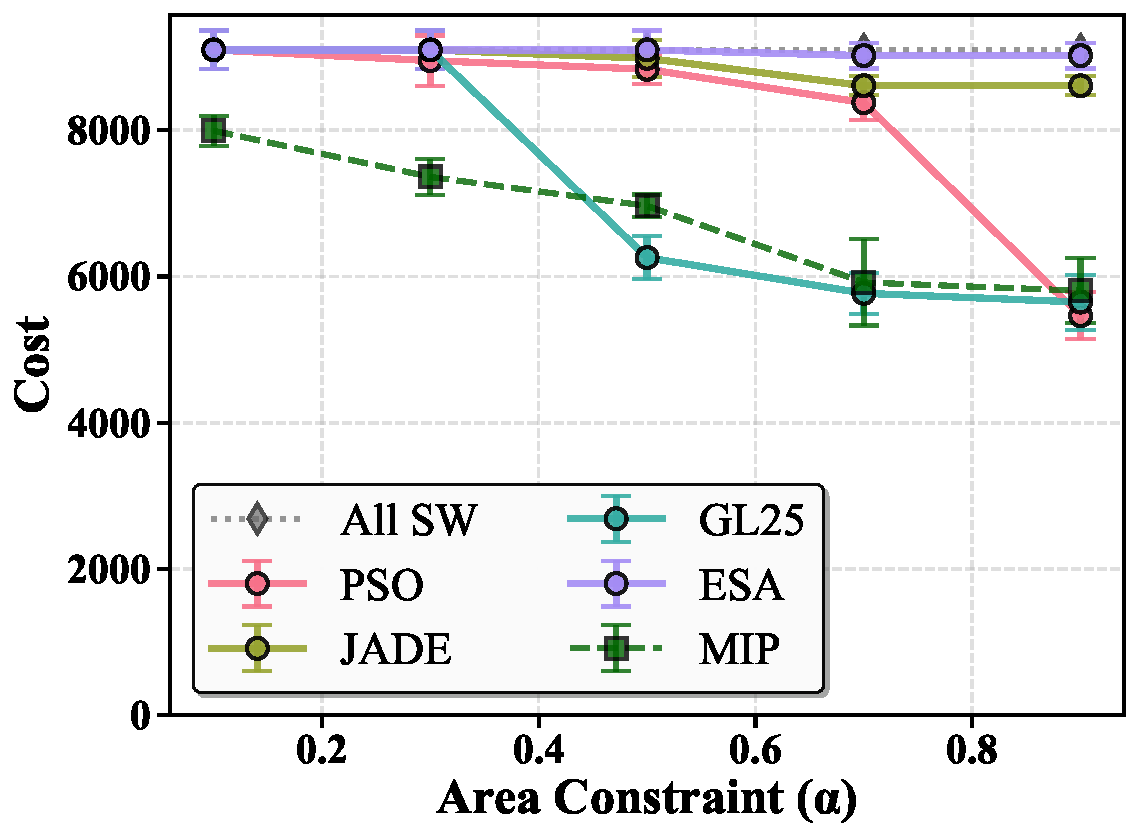
\includegraphics[width=0.32\textwidth]{Figures/meta-heuristic-Figures/sensitivity_methods_vs_area_hw_0.9_strategy_OPTM.pdf}
% }

\end{figure*}



This section presents a detailed sensitivity analysis of four meta-heuristic algorithms (PSO, JADE, GL25, ESA) against two baselines (MIP (expected best), naive all-software (expected worst)) across two optimization strategies and various hardware scale factors ($k \in \{0.1, 0.5, 0.9\}$) and area constraints ($\alpha \in \{0.1, 0.3, 0.5, 0.7, 0.9\}$).

\subsection{Optimization Strategy: ARATO}

At $k=0.1$ where hardware assignment provides a 10$\times$ speedup on average than the corresponding software assignment, the meta-heuristics exhibit significant differences in their performances when they use ARATO optimization strategy. GL25 emerges as the clear winner, achieving competitive performance with respect to the MIP solution. However, PSO is able to find better solution compared to GL25 for tighter area constraints. ESA exhibits unusual behaviour, performing well at intermediate area constraints but reverting to naive performance for more relaxed constraints, suggesting premature convergence or acceptance of local optima. JADE catastrophically fails for this optimization strategy at $k=0.1$, maintaining costs near the naive assignment even at high area budgets (7,942.28 at $\alpha=0.9$).

As hardware advantage diminishes to $k=0.5$, GL25 maintains the best performance. However, it is only able to maintain acceptable margin with MIP for relaxed area constraint. This suggests GL25 excels specifically when substantial hardware resources are available. The collapse of other meta-heuristic performance at $k=0.5$ suggests ARATO's optimization landscape becomes dramatically more disadvantegeous as hardware advantage diminishes.

At $k=0.9$ where hardware provides only marginal speedup, meta-heuristic performance completely collapses for ARATO optimization strategy. 
This universal failure suggests the limited applicability of this optimization strategy when hardware allocation provides negligible benefit.

\subsection{Optimization Strategy: CA}

At $k=0.1$, the CA strategy proves to be more effective compared to ARATO. While GL25 is again the best meta-heuristic, the performance gap with MIP diminishes by a lot, demonstrating that genetic algorithms can exploit this strategy better than ARATO. PSO achieves strong performance at relaxed area constraint. ESA again shows anomalous behaviour, suggesting a fundamental limitation of the meta-heuristic itself in the current problem domain, rather than an issue with the optimization strategy. The struggle of JADE presists, though it performs notably better under CA than ARATO.

At moderate hardware advantage ($k=0.5$), CA strategy maintains better meta-heuristic effectiveness than ARATO at the same scale factor. GL25 achieves an average of 6.04\% performance gap from MIP. This represents a fundamental difference from ARATO; CA strategy maintains effective meta-heuristic exploration even as hardware advantages diminish. PSO achieves the second best performance, followed by ESA, which exhibits its characteristic intermediate-optimum behaviour but struggles at extreme constraints. JADE continues to underperform with a better margin than ARATO, suggesting it navigates the landscape more effectively under CA optimization strategy. 

Even at minimal hardware advantage, CA strategy maintains meta-heuristic viability. The maintained meta-heuristic effectiveness at $k=0.9$ under CA strategy (versus complete collapse under ARATO) demonstrates fundamental differences in objective function landscapes.


\subsection{Fundamental Insights on Optimization Landscape Structure}

The dramatic performance variations across strategies and hardware scales reveal fundamental insights.


% \appendix
\section{Vanilla Partitioning Problem}

\subsection{Problem Definition}

We are given a graph $G=\left(V,E\right)$ with $n$ nodes and $m$ edges. Each node has two node weights $h_i$ and $s_i$ to denote hardware and software costs.
The edges denote communication between the nodes and have associated communication cost $c_{ij}$ for the edge $e$ connecting nodes $i$ and $j$.
The aim is to partition the nodes $V$ into non-overlapping sets $V_S$ and $V_H$ denoting software and hardware nodes respectively; $V=V_H \cup V_S$ and $V_H \cap V_S = \emptyset$.
We denote the set of edges between the two sets by $E_{\cP}$. 
Note that we will only consider communication cost for these edges which are between hardware and software nodes.
The hardware cost for a partition $\cP$ is defined as sum of hardware cost for the nodes belonging to the hardware nodes 
$H_{\cP} = \sum_{v\in V_H}h_v$. Similarly, the software cost for the partition is $S_{\cP} = \sum_{v\in V_S}s_v$.
The communication cost is defined as $C_{\cP} = \sum_{e:(i,j) \in E_\cP} c_{ij}$.

\subsection{Optimization Formulation}
We define binary variable $x_i$ for each node $i \in V$; $x_i=1$ if node $i$ is a software node in partitioning $\cP$, else $x_i=0$ for a hardware node.
Additionally, we denote the edge weighted adjacency matrix for the graph $G$ to be $\bC$, where the element along the $i^{th}$ row and $j^{th}$ column $C_{ij}$ is \[C_{ij}=\begin{cases}c_{ij},~ \textrm{if } e:(i,j) \in E \\ 0,~ \textrm{otherwise}\end{cases}\] Note that $\bC$ is symmetric.
The communication cost for the partition $\cP$ is 
\[C_{\cP} = \sum_{e:(i,j) \in E_\cP} c_{ij}=\sum_{i\in V}\sum_{j\in V}x_i C_{ij} (1-x_j)\]
We can stack the entries $h_i$, $s_i$ and $x_i$ in $n$-length vectors $\bh$, $\bs$ and $\bx$ respectively. For the partition $\cP$, the hardware cost is $H_{\cP}=\bh^T\left(\ones-\bx\right)$, the software cost is $S_{\cP}=\bs^T\bx$, and the communication cost $C_\cP=\left(\ones-\bx\right)\bC\bx$.
The hardware-software partitioning problem can be stated as
\begin{align*}
    \cP^\star = \arg \min & ~ H_\cP\\
    \textrm{s.t.} & ~ S_\cP + C_\cP \leq R_0
\end{align*}
which we can write as
\begin{subequations}
\begin{align}
    \bx^\star = \arg \min & ~ \bh^T\left(\ones - \bx\right)\\
\textrm{s.t.} & ~ \bs^T\bx + \left(\ones - \bx\right)^T\bC\bx \leq R_0\\
& ~ x_i \in \{0,1\},~\forall i=1,2,\cdots,n
\end{align}
\end{subequations}
\begin{relaxation}
    We relax the integer constraint $x_i \in \{0,1\}$ to $0 \leq x_i \leq 1,~ \forall i=1,2,\cdots,n$. 
\end{relaxation}
The relaxed optimization problem is a quadratic constrained linear problem
\begin{subequations}
\begin{align}
    \bx^\star = \arg \min & ~ \bh^T\left(\ones - \bx\right)\\
\textrm{s.t.} & ~ \left(\bs+\bC\ones\right)^T\bx - \bx^T\bC\bx \leq R_0\\
& ~ \zeros \leq \bx \leq \ones
\end{align}
\end{subequations}
Note that $\bC \succeq 0$, and hence, the constraint $\left(\bs+\bC\ones\right)^T\bx - \bx^T\bC\bx \leq R_0$ is non-convex.
We now define $(n+1)\times(n+1)$ matrices
\[\bX=\begin{bmatrix}\bx\bx^T & \bx \\ \bx^T & 1\end{bmatrix} \textrm { and } \bH=\begin{bmatrix}0 & \frac{\bh}{2} \\ \frac{\bh^T}{2} & 0\end{bmatrix}\]
to pose the above problem as a semidefinite program (SDP). Using the linearity and cyclic properties of \emph{trace} of a matrix, we have
\begin{subequations}
    \begin{align}
        & \tr{\bH\bX} = \bh^T\bx\\
        & \tr{\begin{bmatrix}\bC&-\frac{\bs+\bC\ones}{2}\\-\frac{\left(\bs+\bC\ones\right)^T}{2}&R_0\end{bmatrix}\bX} = \bx^T\bC\bx - \left(\bs + \bC\ones\right)^T\bx + R_0
    \end{align}
\end{subequations}
Additionally, we want to add some more constraints to make the problem more tight. These include
\begin{subequations}
    \begin{align}
        \forall i=1,2,\cdots,n \quad &0 \leq x_i \leq 1 ~~ \Rightarrow 0 \leq \be_i^T\bx \leq 1\\
        \forall i=1,2,\cdots,n \quad &X_{ii} = x_i ~~ \Rightarrow \bx^T\bE_{ii}\bx = \be_i^T\bx\\
        \forall i,j=1,2,\cdots,n \quad &X_{ij} \leq x_i ~~ \Rightarrow \bx^T\bE_{ij}\bx \leq \be_i^T\bx\\
        \forall i,j=1,2,\cdots,n \quad &X_{ij} \leq x_j ~~ \Rightarrow \bx^T\bE_{ij}\bx \leq \be_j^T\bx\\
        \forall i,j=1,2,\cdots,n \quad &X_{ij} \geq 0 ~~ \Rightarrow \bx^T\bE_{ij}\bx \geq 0
    \end{align}
    \label{eq:tight}
\end{subequations}
Here, $\bE_{ij}$ denotes a $n\times n$ matrix with all zeros, except the element along the $i^{th}$ row and $j^{th}$ column being $1$, and the vector $\be_i$ denotes the $i^{th}$ column of the $n\times n$ identity matrix.
Using the linearity and cyclic properties of \emph{trace} of a matrix, we have the following identities
\begin{subequations}
    \begin{align}
        &  \tr{\begin{bmatrix}\zeros&\frac{\be_i}{2}\\\frac{\be_i^T}{2}&0\end{bmatrix}\bX} = \be_i^T\bx\\
        & \tr{\begin{bmatrix}\bE_{ij}&-\frac{\be_i}{2}\\-\frac{\be_i^T}{2}&0\end{bmatrix} \bX} = \bx^T\bE_{ij}\bx - \be_i^T\bx
    \end{align}
    \label{eq:identities}
\end{subequations}
The SDP problem is
\begin{subequations}
\begin{align}
\textrm{minimize} & ~ \bh^T\ones - \textrm{Tr}(\bH\bX)\\
\textrm{subject to} & ~ \tr{\begin{bmatrix}\bC&-\frac{\bs+\bC\ones}{2}\\-\frac{\left(\bs+\bC\ones\right)^T}{2}&R_0\end{bmatrix}\bX}\geq 0\\
& ~ 0\leq \tr{\begin{bmatrix}\zeros&\frac{\be_i}{2}\\\frac{\be_i^T}{2}&0\end{bmatrix}\bX}\leq 1,~~ \tr{\begin{bmatrix}\bE_{ii}&-\frac{\be_i}{2}\\-\frac{\be_i^T}{2}&0\end{bmatrix}\bX}= 0, ~~ \forall i\\
& ~ \tr{\begin{bmatrix}\bE_{ij}&-\frac{\be_i}{2}\\-\frac{\be_i^T}{2}&0\end{bmatrix}\bX}\leq 0,~~\tr{\begin{bmatrix}\bE_{ij}&-\frac{\be_j}{2}\\-\frac{\be_j^T}{2}&0\end{bmatrix}\bX}\leq 0 ~~\forall i,j\\
& ~ \tr{\begin{bmatrix}\bE_{ij}&\zeros\\\zeros^T&0\end{bmatrix}\bX}\geq 0~~\forall i,j, ~~ \bX \succeq 0\\
& ~ \textrm{rank}(\bX) = 1
\end{align}
\end{subequations}

\section{Scheduling Constrained Partitioning Problem}

\subsection{Problem Definition}
We are given a graph $G=\left(V,E\right)$ with $n$ nodes and $m$ edges. 
Each node has weights $h_i$ and $s_i$ to denote hardware and software execution times.
Also, each node has an associated hardware area cost $a_i$.
The edges denote communication between the nodes and have associated communication cost $c_{ij}$ for the edge $e$ connecting nodes $i$ and $j$.
The communication delay is taken into account only when the adjacent nodes belong to different partitions.
The aim is to partition the nodes $V$ into non-overlapping sets $V_S$ and $V_H$ denoting software and hardware nodes respectively; $V=V_H \cup V_S$ and $V_H \cap V_S = \emptyset$.
We denote the set of edges between the two sets by $E_{\cP}$. 
Additionally, we need to ensure that software nodes are executed sequentially, while hardware nodes can execute in parallel if their dependent nodes are executed.
Our objective is to minimize the overall execution time given a limited available area for hardware nodes.

\subsection{Optimization Formulation}

\noindent\textbf{Decision variables.}~We define binary variable $x_i=0$ if node $i$ is assigned to hardware partition, $x_i=1$ if assigned to software partition.
We also define binary variable $z_{ij}$ for each edge $e:=\left(i,j\right)\in E$connecting nodes $i$ and $j$. We denote $z_{ij}=1$ if the nodes $i$ and $j$ belong to different partitions.
Let $t_i$ and $f_i$ denote the start and end time of the node $i$. The total execution time of the task graph is denoted by $T$.
We also define binary variable $y_{ij}$ for each pair of nodes $i,j$, $i \neq j$.
This binary variable is used to ensure that if the pair of nodes $i,j$ are assigned to software partition, they need to be executed sequentially; i.e., if $y_{ij}=1$, then node $i$ precedes node $j$, and for $y_{ij}=0$, the opposite happens.
However, we need to ensure that this sequential constraint is activated for only a pair of software nodes.

\noindent\textbf{Hardware area constraint.}~The overall hardware area is constrained by the maximum allowable hardware area $A_{\textrm{max}}$.
\begin{equation}
    \sum_{i=1}^{n}a_i\left(1-x_i\right) \leq A_{\textrm{max}}
    \label{eq:hardware-area}
\end{equation}

\noindent\textbf{Binary edge variable.}~The binary variable $z_{ij}$ and the partition variable $x_i,x_j$ corresponding to the adjacent nodes are related by
\begin{subequations}
    \begin{align}
        &z_{ij} \geq x_i - x_j, \quad &\forall \left(i,j\right) \in E\\
        &z_{ij} \geq x_j - x_i, \quad &\forall \left(i,j\right) \in E\\
        &z_{ij} \leq x_i + x_j, \quad &\forall \left(i,j\right) \in E\\
        &z_{ij} \leq 2 - x_i - x_j, \quad &\forall \left(i,j\right) \in E
    \end{align}
    \label{eq:edge-selection}
\end{subequations}

\noindent\textbf{Execution time constraints.}~The execution time of each node is denoted 
\begin{subequations}
    \begin{align}
        & T \geq f_i, \quad &\forall i \in V\\
        & f_i = t_i + h_i\left(1-x_i\right) + s_ix_i, \quad &\forall i\in V\\
        & f_i + c_{ij}z_{ij} \leq t_j, \quad &\forall \left(i,j\right) \in E
    \end{align}
    \label{eq:exec-time}
\end{subequations}

\noindent\textbf{Sequential execution of software nodes.}We define the following pair of constraints with $M$ being a large positive number.
\begin{subequations}
    \begin{align}
        & f_i \leq t_j + M \left(1 - y_{ij}\right) + M \left(2 - x_i -x_j\right), \quad &\forall i,j \in V, i \neq j\\
        & f_j \leq t_i + M y_{ij} + M \left(2 - x_i -x_j\right), \quad &\forall i,j \in V, i \neq j
    \end{align}
    \label{eq:sw-seq}
\end{subequations}
Note that, the constraints are activated only when $x_i=x_j=1$ or the nodes $i,j$ are both software nodes, when the term $2-x_i-x_j=0$.
For other cases, the constraints are not active since $M$ is sufficiently large.
Once the constraints are activated, the value of $y_{ij}$ denotes the precedence of the software node operations.

The overall optimization problem is
\begin{subequations}
    \begin{align}
        \textrm{minimize} & ~ T\\
        \textrm{subject to} & ~ \left(\ref{eq:hardware-area}\right),\left(\ref{eq:edge-selection}\right),\left(\ref{eq:exec-time}\right),\left(\ref{eq:sw-seq}\right)
    \end{align}
\end{subequations}

\FloatBarrier
\bibliographystyle{acm}
\bibliography{ref}

\section{Appendix}

\noindent \textbf{Notations:} Table~\ref{tab:Notation} summarizes the main notations used in this paper.

\begin{table}[!htbp]
\caption{Main notations.}
\label{tab:Notation}
\centering
\resizebox{1.0\linewidth}{!}{
\begin{tabular}{l l l}
\toprule
$\gG(\gV,\gE)$ & $\triangleq$ & Task graph \\
$(j,i)$ & $\triangleq$ & Dependency edge $j \rightarrow i$ \\
$t_i^{sw},\,t_i^{hw}$ & $\triangleq$ & SW/HW execution costs \\
$A_i,\,A_{\max}$ & $\triangleq$ & Node area and area budget \\
$C_{ji}$ & $\triangleq$ & Communication cost on $(j,i)$ \\

$\vp,\tilde{\vp},\hat{\vp}$ & $\triangleq$ & Discrete, relaxed, and decoded placements \\
$p_i,\tilde{p}_i,\hat{p}_i$ & $\triangleq$ & Corresponding node assignments \\
$\pi^{sw},\,\tilde{\vpi}^{sw}$ & $\triangleq$ & Discrete and relaxed software order \\
$\pi_{\mathrm{learn}}^{sw},\,\pi_{\mathrm{static}}^{sw}$ & $\triangleq$ & Learned and static software orders \\

$\vs,\vf$ & $\triangleq$ & Discrete start and finish times \\
$\tilde{\vs},\tilde{\vf}$ & $\triangleq$ & Relaxed start and finish times \\
$M(\vp,\pi^{sw})$ & $\triangleq$ & Discrete makespan \\
$\widetilde{M}(\tilde{\vp},\tilde{\vpi}^{sw})$ & $\triangleq$ & Relaxed makespan \\
$\tilde{t}_i(\tilde{\vp}),\,\tilde{c}_{ji}(\tilde{\vp})$ & $\triangleq$ & Relaxed execution and communication \\
$\mathrm{SMax}_{\beta}(\cdot)$ & $\triangleq$ & Smooth maximum \\
\bottomrule
\end{tabular}
}
\end{table}


% \section{Illustrative 6-node example.}
\label{app:illustration}

Let us consider the task graph of Figure~\ref{fig:demosoftmakespan}. The numerical values below are illustrative demo values used only to explain the differentiable soft scheduler.

\begin{figure}[!htbp]
\centering
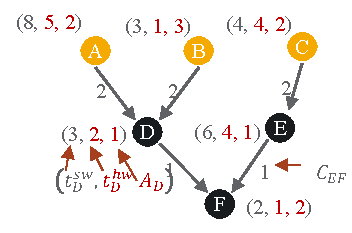
\includegraphics[width=0.52\linewidth]{Figures/methods/demosoftmakespan.pdf}
\caption{Illustrative 6-node fork-join task graph used to explain the differentiable soft scheduler. Each node is annotated with $(t_i^{sw}, t_i^{hw}, A_i)$ and each edge label denotes communication cost.}
\label{fig:demosoftmakespan}
\end{figure}

The graph has dependencies
\[
A \rightarrow D,\quad B \rightarrow D,\quad C \rightarrow E,\quad D \rightarrow F,\quad E \rightarrow F.
\]

For this example, the placement head predicts
\begin{equation}
\tilde{\vp}=[0.05,\,0.05,\,0.05,\,0.95,\,0.95,\,0.95]^\top,
\end{equation}
for tasks $(A,B,C,D,E,F)$, indicating that $A,B,C$ are nearly assigned to software, while $D,E,F$ are nearly assigned to hardware. The ordering head predicts
\begin{equation}
\tilde{\vpi}^{sw}=[0.00,\,-1.00,\,1.00,\,-0.50,\,-0.75,\,-0.25]^\top.
\end{equation}

Using the task costs in Figure~\ref{fig:demosoftmakespan}, the relaxed execution times are
\begin{align}
\tilde t_A &= 0.05\cdot 5 + 0.95\cdot 8 = 7.85, &
\tilde t_B &= 0.05\cdot 1 + 0.95\cdot 3 = 2.90, \\
\tilde t_C &= 0.05\cdot 4 + 0.95\cdot 4 = 4.00, &
\tilde t_D &= 0.95\cdot 2 + 0.05\cdot 3 = 2.05, \\
\tilde t_E &= 0.95\cdot 4 + 0.05\cdot 6 = 4.10, &
\tilde t_F &= 0.95\cdot 1 + 0.05\cdot 2 = 1.05.
\end{align}
Similarly, the soft communication on the cut edges is
\begin{equation}
\tilde c_{AD}=\tilde c_{BD}=\tilde c_{CE}=|0.05-0.95|\cdot 2 = 1.8,
\end{equation}
while $\tilde c_{DF}=\tilde c_{EF}=0$ because the corresponding communication cost is $0$.

\paragraph{\textbf{Step 1: ordering head \(\rightarrow\) Sinkhorn matrix \(\rightarrow\) expected ranks.}}
Using the score-to-position compatibility
\begin{equation}
L_{ai} = -\frac{(\tilde{\pi}_i^{sw}-u_a)^2}{\tau_o},
\qquad
u_a = 1-\frac{2a}{n-1},
\quad a=0,\ldots,n-1,
\end{equation}
Sinkhorn normalization yields the soft permutation matrix
\begingroup
\setlength{\arraycolsep}{3pt}
\begin{equation}
\scriptsize
\mP^{sw}\approx
\begin{bmatrix}
0.181 & 0.002 & 0.695 & 0.029 & 0.008 & 0.084\\
0.332 & 0.015 & 0.257 & 0.120 & 0.047 & 0.229\\
0.271 & 0.060 & 0.043 & 0.218 & 0.128 & 0.280\\
0.143 & 0.155 & 0.005 & 0.255 & 0.224 & 0.219\\
0.056 & 0.302 & 0.000 & 0.223 & 0.291 & 0.128\\
0.017 & 0.467 & 0.000 & 0.155 & 0.302 & 0.060
\end{bmatrix},
\end{equation}
\endgroup
where rows correspond to positions \(a=0,\ldots,5\) and columns correspond to tasks \((A,B,C,D,E,F)\).

The expected ranks are then
\begin{equation}
\tilde r_i=\sum_{a=0}^{n-1} a\,\mP^{sw}_{ai},
\end{equation}
which gives
\begin{equation}
\tilde{\vr}^{sw}\approx
[1.613,\;4.141,\;0.357,\;2.986,\;3.649,\;2.258]^\top.
\end{equation}
Hence the induced global soft order is
\[
C \prec A \prec F \prec D \prec E \prec B,
\]
and the induced software order over the three nearly-software tasks is
\[
C \prec A \prec B.
\]

\paragraph{\textbf{Step 2: expected ranks \(\rightarrow\) before matrix.}}
Using the rank-sigmoid approximation,
\begin{equation}
B^{sw}_{ji}
=
\sigma\!\left(\frac{\tilde r_i-\tilde r_j}{\tau_r}\right),
\qquad
B^{sw}_{ii}=0,
\end{equation}
we obtain the soft before matrix
\begingroup
\setlength{\arraycolsep}{3pt}
\begin{equation}
\scriptsize
\mB^{sw}\approx
\begin{bmatrix}
0     & 0.999 & 0.027 & 0.981 & 0.997 & 0.863\\
0.001 & 0     & 0     & 0.036 & 0.197 & 0.005\\
0.973 & 1.000 & 0     & 0.999 & 1.000 & 0.996\\
0.019 & 0.964 & 0.001 & 0     & 0.869 & 0.111\\
0.003 & 0.803 & 0     & 0.131 & 0     & 0.018\\
0.137 & 0.995 & 0.004 & 0.889 & 0.982 & 0
\end{bmatrix},
\end{equation}
\endgroup
so, for example,
\[
B^{sw}_{CA}=0.973,\qquad B^{sw}_{CB}=1.000,\qquad B^{sw}_{AB}=0.999,
\]
which strongly supports the order \(C \prec A \prec B\).

\paragraph{\textbf{Step 3: gate using placement probabilities.}}
Since ordering matters only when both tasks are likely to execute in software, we use the gate
\begin{equation}
\mG^{sw}=(1-\tilde{\vp})(1-\tilde{\vp})^\top
=
\begin{bmatrix}
0.9025\,\mathbf{1}_{3\times 3} & 0.0475\,\mathbf{1}_{3\times 3}\\
0.0475\,\mathbf{1}_{3\times 3} & 0.0025\,\mathbf{1}_{3\times 3}
\end{bmatrix},
\end{equation}
because \(1-\tilde p_i=0.95\) for \(A,B,C\) and \(1-\tilde p_i=0.05\) for \(D,E,F\).

The effective resource-order matrix is
\begin{equation}
\mR^{sw}=\mB^{sw}\odot \mG^{sw},
\end{equation}
which gives
\begingroup
\setlength{\arraycolsep}{3pt}
\begin{equation}
\scriptsize
\mR^{sw}\approx
\begin{bmatrix}
0     & 0.902 & 0.024 & 0.047 & 0.047 & 0.041\\
0.001 & 0     & 0     & 0.002 & 0.009 & 0    \\
0.878 & 0.902 & 0     & 0.047 & 0.047 & 0.047\\
0.001 & 0.046 & 0     & 0     & 0.002 & 0    \\
0     & 0.038 & 0     & 0     & 0     & 0    \\
0.006 & 0.047 & 0     & 0.002 & 0.002 & 0
\end{bmatrix}.
\end{equation}
\endgroup
In particular,
\[
R^{sw}_{AB}=0.902,\qquad
R^{sw}_{CA}=0.878,\qquad
R^{sw}_{CB}=0.902,
\]
which strongly prefers \(C\) before \(A\) and \(B\), and \(A\) before \(B\).

\paragraph{\textbf{Step 4: DAG readiness and software readiness.}}
To make the effect concrete, we use the hard-order interpretation induced by the soft ranks. For the nearly-software tasks \(A,B,C\), the DAG-readiness values are
\[
s_A^{dag}=s_B^{dag}=s_C^{dag}=0,
\]
since they are source nodes. Thus, their ordering is driven entirely by the software-readiness term. Under the induced software order \(C\prec A\prec B\), we obtain approximately
\begin{align}
s_C^{sw} &\approx 0, &
\tilde s_C &\approx \max(s_C^{dag},s_C^{sw}) = 0, &
\tilde f_C &\approx 0 + 4.00 = 4.00,\\
s_A^{sw} &\approx \tilde f_C = 4.00, &
\tilde s_A &\approx \max(0,4.00) = 4.00, &
\tilde f_A &\approx 4.00 + 7.85 = 11.85,\\
s_B^{sw} &\approx \tilde f_A = 11.85, &
\tilde s_B &\approx \max(0,11.85) = 11.85, &
\tilde f_B &\approx 11.85 + 2.90 = 14.75.
\end{align}

Now consider the hardware tasks. Since \(D\) depends on both \(A\) and \(B\),
\begin{equation}
s_D^{dag}\approx \max(\tilde f_A+\tilde c_{AD},\,\tilde f_B+\tilde c_{BD})
=
\max(11.85+1.8,\;14.75+1.8)
=
16.55,
\end{equation}
and \(s_D^{sw}\approx 0\), so
\[
\tilde s_D\approx 16.55,\qquad
\tilde f_D\approx 16.55+2.05=18.60.
\]
Similarly, since \(E\) depends on \(C\),
\begin{equation}
s_E^{dag}\approx \tilde f_C+\tilde c_{CE}=4.00+1.8=5.80,
\end{equation}
hence
\[
\tilde s_E\approx 5.80,\qquad
\tilde f_E\approx 5.80+4.10=9.90.
\]
Finally, \(F\) depends on both \(D\) and \(E\), so
\begin{equation}
s_F^{dag}\approx \max(\tilde f_D,\tilde f_E)=\max(18.60,9.90)=18.60,
\end{equation}
which yields
\[
\tilde s_F\approx 18.60,\qquad
\tilde f_F\approx 18.60+1.05=19.65.
\]
Thus, the induced relaxed makespan is approximately
\[
L_{\mathrm{soft\mbox{-}makespan}} \approx 19.65.
\]

\paragraph{\textbf{Why \(C\prec A\prec B\) is better than \(A\prec B\prec C\).}}
If the software order were instead \(A\prec B\prec C\), then the same hard-order approximation gives
\[
\tilde f_A\approx 7.85,\qquad
\tilde f_B\approx 10.75,\qquad
\tilde f_C\approx 14.75.
\]
Therefore,
\[
s_D^{dag}\approx \max(7.85+1.8,\;10.75+1.8)=12.55,
\qquad
\tilde f_D\approx 14.60,
\]
while
\[
s_E^{dag}\approx 14.75+1.8=16.55,
\qquad
\tilde f_E\approx 20.65.
\]
This delays the \(C\rightarrow E\rightarrow F\) branch, and hence
\[
s_F^{dag}\approx \max(14.60,\;20.65)=20.65,
\qquad
\tilde f_F\approx 21.70.
\]
Thus,
\[
\mathrm{makespan}(C\prec A\prec B)\approx 19.65
\;<\;
\mathrm{makespan}(A\prec B\prec C)\approx 21.70.
\]

The reason is that the \(C\rightarrow E\) branch is the slower downstream branch: once \(C\) finishes, task \(E\) still needs about \(4.10\) units to complete, whereas the \(A,B\rightarrow D\) branch needs only about \(2.05\) units after both \(A\) and \(B\) finish. Prioritizing \(C\) earlier therefore reduces the final critical path.

\paragraph{\textbf{Why DAG-only readiness is insufficient.}}
Without the ordering head, a scheduler based only on DAG readiness cannot distinguish among the ready source tasks \(A,B,C\), because all three have
\[
s_A^{dag}=s_B^{dag}=s_C^{dag}=0.
\]
Any topological order, such as \(A\prec B\prec C\) or \(C\prec A\prec B\), is valid from the precedence perspective alone. However, these orders produce different software serialization patterns and different makespans. The ordering head resolves this ambiguity by producing a structured pairwise precedence matrix, which allows the soft scheduler to model resource-induced serialization in addition to DAG constraints.

% \pagebreak
\section{Pseudocode}

\begin{algorithm}[!htbp]
\caption{Training of \diffgnn}
\label{alg:diffgnn_trainingapp}
\KwIn{Task graph $\gG=(\gV,\gE)$, epochs $T$, area budget $A_{\max}$}
\KwIn{Area penalty weight $\lambda_a$, ordering temperature $\tau_o$, smooth-max parameter $\beta$}
Initialize model parameters $\theta$\;

\For{$t=1,\dots,T$}{
    Construct node and edge features $\mF,\mE$\;
    Predict relaxed placement and ordering scores
    $\vp,\vq^{sw} \gets \mathrm{GNN}_{\theta}(\gG,\mF,\mE)$,
    where $\vp\in[0,1]^n$ and $\vq^{sw}\in\mathbb{R}^n$\;

    Convert ordering scores to a soft resource-order matrix\;
    $\mP^{sw}\gets \mathrm{Sinkhorn}(\vq^{sw}/\tau_o)$\;
    $\mB^{sw}\gets \mathrm{BeforeMatrix}(\mP^{sw})$\;
    $\forall (j,i)\in\gV\times\gV:\;
    B^{res}_{j,i}\gets B^{sw}_{j,i}(1-p_j)(1-p_i)$\;

    Compute soft execution and communication costs\;
    $\forall i\in\gV:\;
    \tilde{t}_i \gets p_i t_i^{hw} + (1-p_i)t_i^{sw}$\;
    $\forall (j,i)\in\gE:\;
    \tilde{c}_{ji} \gets |p_j-p_i|\,c_{ji}$\;

    Process nodes in topological order\;
    \ForEach{$i\in\gV$}{
        $R_{\mathrm{dag}}(i)\gets
        \mathrm{SMax}_{\beta}\!\Big(\{0\}\cup\{f_j+\tilde{c}_{ji}: j\in\mathrm{pred}(i)\}\Big)$\;

        $R_{\mathrm{res}}(i)\gets
        \mathrm{SMax}_{\beta}\!\Big(\{0\}\cup\{f_j+\alpha\log(B^{res}_{j,i}+\varepsilon): j\neq i\}\Big)$\;

        $s_i \gets \mathrm{SMax}_{\beta}\!\big(R_{\mathrm{dag}}(i), R_{\mathrm{res}}(i)\big)$\;
        $f_i \gets s_i+\tilde{t}_i$\;
    }

    $L_{\mathrm{soft\mbox{-}makespan}}
    \gets
    \mathrm{SMax}_{\beta}\!\big(\{f_i:i\in\gV_{\mathrm{sink}}\}\big)$\;

    $L_{\mathrm{exec}} \gets \sum_{i\in\gV}\tilde{t}_i$\;
    $L_{\mathrm{comm}} \gets \sum_{(j,i)\in\gE}\tilde{c}_{ji}$\;
    $L_{\mathrm{area}}
    \gets
    \left[\max\!\left(0,\sum_{i\in\gV}p_iA_i-A_{\max}\right)\right]^2$\;

    $L \gets L_{\mathrm{makespan}} + L_{\mathrm{exec}} + L_{\mathrm{comm}} + \lambda_a L_{\mathrm{area}}+ L_\mathrm{reg}$\;

    Update $\theta$ via backpropagation\;
}
\end{algorithm}

\begin{algorithm}[!htbp]
\caption{Decoding and Refinement}
\label{alg:diffgnn_inferenceapp}
\KwIn{Graph $\gG$, trained model, area budget $A_{\max}$, thresholds $\mathcal{T}$}
\KwOut{Best partition $\vx^\star$}

Compute $\vp$, $\vq^{sw}$\;

Initialize $\vx^\star \gets \emptyset$, $M^\star \gets +\infty$\;

\For{$\tau_d \in \mathcal{T}$}{
    Decode $\vx$: $x_i = \mathbb{I}[p_i \ge \tau_d]$\;

    \While{$\sum_i x_i A_i > A_{\max}$}{
        Move a hardware node to software\;
    }

    Refine/improve $\vx$ (local search)\;    
    Compute makespan $M(\vx)$ using LSSP\;

    \If{$M(\vx) < M^\star$}{
        $\vx^\star \gets \vx$, \quad $M^\star \gets M(\vx)$\;
    }
}

\Return{$\vx^\star$}\;
\end{algorithm}


% \newpage\pagebreak

% \begin{figure*}[!t]
% \centering
% \begin{tikzpicture}[
%     font=\small,
%     >=Latex,
%     flow/.style={->, draw=black, line width=0.9pt},
%     line/.style={draw=black, line width=0.8pt},
%     thinann/.style={draw=black, line width=0.45pt},
%     task/.style={circle, draw=black!75, line width=0.7pt, minimum size=4.5mm, inner sep=0pt, fill=white},
%     tuple/.style={font=\scriptsize, text=black!80},
%     edgew/.style={font=\scriptsize, inner sep=1pt, fill=white, text=black!80},
%     gnn/.style={draw=black!75, rounded corners=2.2mm, line width=0.85pt, fill=gray!8,
%                 minimum width=1.95cm, minimum height=0.88cm, align=center, inner sep=3pt},
%     box/.style={draw=black!75, line width=0.85pt, fill=gray!8, inner sep=4pt, align=center},
%     topbrace/.style={decorate, decoration={brace, amplitude=4pt, raise=2pt}, draw=black, line width=0.8pt},
%     stagebox/.style={draw=black!75, rounded corners=2.2mm, line width=0.9pt, inner sep=6pt}
% ]

% % =========================================================
% % Input preparation
% % =========================================================
% \node[task] (A) at (0.90,2.90) {A};
% \node[task] (B) at (1.65,2.90) {B};
% \node[task] (C) at (2.40,2.90) {C};
% \node[task] (D) at (1.18,2.05) {D};
% \node[task] (E) at (2.08,2.05) {E};
% \node[task] (F) at (1.60,1.18) {F};

% % node tuples relative to nodes
% \node[tuple, above=3pt of A] {(8, 5, 2)};
% \node[tuple, above=3pt of B] {(3, 1, 3)};
% \node[tuple, above=3pt of C] {(4, 4, 2)};
% \node[tuple, left=3pt of D] {(3, 2, 1)};
% \node[tuple, right=3pt of E] {(6, 4, 1)};
% \node[tuple, right=4pt of F] {(2, 1, 2)};

% % DAG edges
% \draw[flow] (A) -- node[edgew, pos=0.57, left=0.5pt] {2} (D);
% \draw[flow] (B) -- node[edgew, pos=0.52, right=0.5pt] {2} (D);
% \draw[flow] (C) -- node[edgew, pos=0.55, right=0.5pt] {2} (E);
% \draw[flow] (D) -- (F);
% \draw[flow] (E) -- node[edgew, pos=0.56, right=0.5pt] {1} (F);

% % thin feature pointers
% \node[font=\scriptsize, text=black!80, anchor=west] (dfeat) at (0.10,0.34)
% {$(t_D^{\mathrm{sw}},\,t_D^{\mathrm{hw}},\,A_D)$};
% \draw[thinann] (0.55,0.57) -- (1.00,1.63);
% \draw[thinann] (0.95,0.57) -- (1.15,1.63);
% \draw[thinann] (1.35,0.57) -- (1.29,1.63);

% \node[font=\scriptsize, text=black!80, anchor=west] at (2.68,1.16) {$C_{EF}$};
% \draw[thinann] (2.58,1.16) -- (1.92,1.16);

% % =========================================================
% % Training: GNN + heads + loss
% % =========================================================
% \node[gnn] (gnn) at (4.65,2.05) {$\mathit{GNN}_{\theta}(\gG,\mF,\mE)$};

% % graph -> gnn
% \draw[flow] (2.95,2.05) -- (gnn.west);

% % heads
% \node[box, anchor=west, minimum width=2.10cm, minimum height=0.98cm] (place) at (6.35,2.58)
% {Placement head\\[1pt]$\tilde{\vp}\in[0,1]^n$};

% \node[box, anchor=west, minimum width=2.10cm, minimum height=0.98cm] (order) at (6.35,1.22)
% {Ordering head\\[1pt]$\tilde{\vpi}^{\mathrm{sw}}\in[-1,1]^n$};

% % gnn -> heads
% \coordinate (split1) at ($(gnn.east)+(0.30,0)$);
% \draw[line] (gnn.east) -- (split1);
% \draw[flow] (split1) |- (place.west);
% \draw[flow] (split1) |- (order.west);

% % loss
% \node[box, anchor=west, text width=3.20cm, font=\scriptsize] (loss) at (9.60,2.00)
% {%
% $L \leftarrow L_{\mathrm{makespan}}(\tilde{\vp},\tilde{\vpi}^{\mathrm{sw}})$\\[1pt]
% $+\lambda_e L_{\mathrm{exec}}(\tilde{\vp}) + \lambda_c L_{\mathrm{comm}}(\tilde{\vp})$\\[1pt]
% $+\lambda_a L_{\mathrm{area}}(\tilde{\vp}) + L_{\mathrm{reg}}(\tilde{\vp},\tilde{\vpi}^{\mathrm{sw}})$%
% };

% % heads -> loss
% \coordinate (split2) at ($(loss.west)+(-0.28,0)$);
% \draw[line] (split2) -- (loss.west);
% \draw[flow] (place.east) -- ++(0.20,0) |- (split2);
% \draw[flow] (order.east) -- ++(0.20,0) |- (split2);

% % enclosing training box
% \node[stagebox, fit=(gnn)(place)(order)(loss)] (trainbox) {};

% % =========================================================
% % Inference and post-processing
% % =========================================================
% \node[box, anchor=west, align=left, text width=4.10cm, font=\scriptsize] (refine) at (14.00,2.0)
% {%
% $\bullet$~Placement $\vp \leftarrow (\tilde{\vp}\geq \tau)$\\
% \hspace*{1.2em}$\circ$~repair area if required\\[2pt]
% $\bullet$~SW order\\
% \hspace*{1.2em}$\circ$~learned order $\vpi_{\mathrm{learn}}^{\mathrm{sw}} \leftarrow \tilde{\vpi}^{\mathrm{sw}}$\\
% \hspace*{1.2em}$\circ$~static order $\vpi_{\mathrm{static}}^{\mathrm{sw}} \leftarrow \text{critical path}$\\[2pt]
% $\bullet$~Refine placement $\vp$\\
% \hspace*{1.2em}$\circ$~local search using $\vpi_{\mathrm{learn}}^{\mathrm{sw}}/\vpi_{\mathrm{static}}^{\mathrm{sw}}$\\[2pt]
% $\bullet$~Select best $(\vp,\vpi^{\mathrm{sw}})$%
% };

% % loss -> inference
% \draw[flow] (loss.east) -- (refine.west);

% % =========================================================
% % Top braces
% % =========================================================
% \draw[topbrace] (0.20,4.32) -- (2.55,4.32)
% node[midway, yshift=10pt, font=\small, text=black!80]
% {Input preparation};

% \draw[topbrace] (2.95,4.32) -- (13.15,4.32)
% node[midway, yshift=10pt, font=\small, text=black!80]
% {Training};

% \draw[topbrace] (13.65,4.32) -- (18.85,4.32)
% node[midway, yshift=10pt, font=\small, text=black!80]
% {Inference \& post-processing};

% \path[use as bounding box] (0.00,0.00) rectangle (19.05,4.72);
% \end{tikzpicture}
% \end{figure*}



\end{document}


